% % \DocumentMetadata{testphase={phase-III,math,table}}
\documentclass[12pt]{article}
% ================= DOCUMENT CLASS & LANGUAGE =================
% \documentclass[12pt]{article} % Moved to main.tex

% ================= TABLE OF CONTENTS (Very Early) =================
\usepackage[titles]{tocloft}

\usepackage[T5]{fontenc}
\usepackage[utf8]{inputenc}
\usepackage[vietnamese,english]{babel}

% ================= ENCODING & FONTS =================
\usepackage{lmodern}
\usepackage{amsfonts}
\usepackage{amssymb}
\usepackage{amsmath}

% ================= LAYOUT & GEOMETRY =================
\usepackage[left=2.55cm,right=2.5cm,top=2cm,bottom=2cm]{geometry}
\usepackage{pdflscape}
\setlength{\parindent}{30pt}
\usepackage{indentfirst}
\usepackage[parfill]{parskip}
\usepackage{setspace}

% ================= TYPOGRAPHY & SECTIONS =================
\usepackage{titlesec}
\titlespacing{\section}{0pt}{12pt plus 2pt minus 2pt}{8pt plus 2pt minus 2pt}
\titlespacing{\subsection}{0pt}{10pt plus 2pt minus 2pt}{6pt plus 2pt minus 2pt}
\setcounter{tocdepth}{3}
\usepackage{svg}



% ================= BIBLIOGRAPHY =================
% \usepackage{csquotes}
% \usepackage{biblatex}
% \DeclareLanguageMapping{vietnamese}{english}

% ================= LISTS & ENUMERATIONS =================
\usepackage{enumitem}
\usepackage{pifont}

% ================= GRAPHICS & TIKZ =================
\usepackage{graphicx}
\usepackage{tikz}
\usetikzlibrary{calc,shapes.geometric,arrows.meta,positioning}
\usepackage{forest}

% ================= TABLES & ARRAYS =================
\usepackage{array}
\usepackage{tabularx}
\usepackage{booktabs}
\usepackage{longtable}

% ================= FLOATING OBJECTS =================
\usepackage{float}
\usepackage{placeins}
\usepackage{subcaption}

% ================= CODE & LISTINGS =================
\usepackage{listings}
\usepackage{algorithm,algpseudocode}

% ================= HEADERS & FOOTERS =================
\usepackage{fancyhdr}

% ================= HYPERLINKS (Last) =================
\usepackage[dvipsnames]{xcolor}
\usepackage{hyperref}
\hypersetup{
    colorlinks=true,
    linkcolor=black,
    urlcolor=blue,
    citecolor=black,
    filecolor=black
}

% ================= BOXES (After Hyperref) =================
\usepackage[most]{tcolorbox}


% for drawing
\usepackage{tikz}
\usetikzlibrary{shapes, arrows, positioning, calc}
\usepackage{float} % Để giữ hình nằm đúng chỗ

\usetikzlibrary{shapes, arrows, positioning, fit, calc, shadows}

\renewcommand{\tabularxcolumn}[1]{m{#1}}
\usepackage{tikz}
\usetikzlibrary{shapes.geometric, arrows.meta, positioning, calc, fit, backgrounds}
\usepackage{adjustbox}

% ================= COLOR DEFINITIONS =================
\definecolor{codegreen}{rgb}{0,0.6,0}
\definecolor{codegray}{rgb}{0.5,0.5,0.5}
\definecolor{codepurple}{rgb}{0.58,0,0.82}
\definecolor{backcolour}{rgb}{0.95,0.95,0.92}

% ================= LISTINGS STYLE =================
\lstdefinestyle{mystyle}{
    backgroundcolor=\color{backcolour},
    commentstyle=\color{codegreen},
    keywordstyle=\color{magenta},
    numberstyle=\tiny\color{codegray},
    stringstyle=\color{codepurple},
    basicstyle=\ttfamily\footnotesize,
    breaklines=true,
    captionpos=b,
    keepspaces=true,
    numbers=left,
    numbersep=5pt,
    showspaces=false,
    showstringspaces=false,
    tabsize=2
}
\lstset{style=mystyle}

% ================= TCOLORBOX STYLES =================
\tcbset{
    myinputbox/.style={
        colback=blue!10,
        colframe=blue!50!black,
        coltitle=white,
        title=Input,
        fonttitle=\bfseries,
        sharp corners=south,
        boxrule=0.8mm,
        arc=2mm,
        top=1mm,
        bottom=1mm,
        left=1mm,
        right=1mm
    },
    myoutputbox/.style={
        colback=green!10,
        colframe=green!50!black,
        coltitle=white,
        title=Output,
        fonttitle=\bfseries,
        sharp corners=south,
        boxrule=0.8mm,
        arc=2mm,
        top=1mm,
        bottom=1mm,
        left=1mm,
        right=1mm
    }
}



\begin{document}
\begin{center}
    \color{BlueViolet}

     \textbf{\newline\newline}
    \vspace{6pt}
    \large
    \textbf{\\TRƯỜNG ĐẠI HỌC KHOA HỌC TỰ NHIÊN}
    

    
    \vspace{6pt}
    \large
    \textbf{\\KHOA CÔNG NGHỆ THÔNG TIN}

    \vspace{6pt}
    \large
    \textbf{\\MÔN PHÂN TÍCH THIẾT KẾ HỆ THỐNG THÔNG TIN}
   
\end{center}

\begin{center}
    
\includegraphics[scale=0.25,alt={Logo of HCMUS}]{images/Logo_HCMUS.png}
    \color{BlueViolet}
    
   \large
   \textbf{BÁO CÁO ĐỒ ÁN}
    \vspace{25pt}\\

    \color{BlueViolet}
    \textbf{GIẢNG VIÊN:} 
    \color{Black}
    \\ ThS. Nguyễn Ngọc Minh Châu
    \vspace{15pt}\\


    \color{BlueViolet}
    \textbf{SINH VIÊN (NHÓM 6):}
    \color{Black}
     \\ {Lê Nguyên Thảo - 23127118}
    \\ {Đởm Quang Minh Triết - 23127131}
    \\ {Đinh Đại Vũ - 23127144}
    \\ {Nguyễn Đăng Phôn - 23127451}
    \vspace{25pt}\\

\end{center}

\begin{tikzpicture}[remember picture,overlay,inner sep=0,outer sep=0]
     \draw[blue!70!black,line width=4pt] ([xshift=-1.5cm,yshift=-2cm]current page.north east) coordinate (A)--([xshift=1.5cm,yshift=-2cm]current page.north west) coordinate(B)--([xshift=1.5cm,yshift=2cm]current page.south west) coordinate (C)--([xshift=-1.5cm,yshift=2cm]current page.south east) coordinate(D)--cycle;

     \draw ([yshift=0.5cm,xshift=-0.5cm]A)-- ([yshift=0.5cm,xshift=0.5cm]B)--
     ([yshift=-0.5cm,xshift=0.5cm]B) --([yshift=-0.5cm,xshift=-0.5cm]B)--([yshift=0.5cm,xshift=-0.5cm]C)--([yshift=0.5cm,xshift=0.5cm]C)--([yshift=-0.5cm,xshift=0.5cm]C)-- ([yshift=-0.5cm,xshift=-0.5cm]D)--([yshift=0.5cm,xshift=-0.5cm]D)--([yshift=0.5cm,xshift=0.5cm]D)--([yshift=-0.5cm,xshift=0.5cm]A)--([yshift=-0.5cm,xshift=-0.5cm]A)--([yshift=0.5cm,xshift=-0.5cm]A);


     \draw ([yshift=-0.3cm,xshift=0.3cm]A)-- ([yshift=-0.3cm,xshift=-0.3cm]B)--
     ([yshift=0.3cm,xshift=-0.3cm]B) --([yshift=0.3cm,xshift=0.3cm]B)--([yshift=-0.3cm,xshift=0.3cm]C)--([yshift=-0.3cm,xshift=-0.3cm]C)--([yshift=0.3cm,xshift=-0.3cm]C)-- ([yshift=0.3cm,xshift=0.3cm]D)--([yshift=-0.3cm,xshift=0.3cm]D)--([yshift=-0.3cm,xshift=-0.3cm]D)--([yshift=0.3cm,xshift=-0.3cm]A)--([yshift=0.3cm,xshift=0.3cm]A)--([yshift=-0.3cm,xshift=0.3cm]A);

\end{tikzpicture}
\newpage
\renewcommand{\contentsname}{\textbf{Mục lục}}

\tableofcontents

\newpage

\renewcommand{\listfigurename}{Danh sách hình ảnh}
\renewcommand{\listtablename}{Danh sách bảng}

\listoffigures
\listoftables


\newpage
\newpage
\section*{Danh sách thành viên nhóm}

\begin{table}[h!]
    \centering
    \small
    \renewcommand{\arraystretch}{1.5}
    \begin{tabularx}{\textwidth}{|c|l|c|X|c|}
        \hline
        \textbf{STT} & \textbf{Họ \& Tên} & \textbf{MSSV} & \textbf{Email} & \textbf{Đóng góp} \\ \hline
        1 & Lê Nguyên Thảo & 23127118 & lnthao23@clc.fitus.edu.vn & 25\% \\ \hline
        2 & Đởm Quang Minh Triết & 23127131 & dqmtriet23@clc.fitus.edu.vn & 25\% \\ \hline
        3 & Đinh Đại Vũ & 23127144 & ddvu23@clc.fitus.edu.vn & 25\% \\ \hline
        4 & Nguyễn Đăng Phôn & 23127451 & ndphon23@clc.fitus.edu.vn & 25\% \\ \hline
    \end{tabularx}
    \caption{Danh sách thành viên nhóm}
\end{table}

\vspace{1cm}
\renewcommand{\arraystretch}{1.5}
\section*{Danh sách phân công}

\begin{table}[H]
    \centering
    \resizebox{\textwidth}{!}{
        \begin{tabular}{|c|l|l|c|c|}
        \hline
        \textbf{STT} & \textbf{Công việc} & \textbf{Phụ trách} & \textbf{Student ID} & \textbf{Mức độ hoàn thành} \\ \hline
        1 &  &
        Lê Nguyên Thảo & 23127118 & 100\% \\ \hline
        
        2 &  &
        Đởm Quang Minh Triết & 23127131 & 100\% \\ \hline

        3 &  &
        Đinh Đại Vũ & 23127144 & 100\% \\ \hline

        4 &  &
        Nguyễn Đăng Phôn & 23127451 & 100\% \\ \hline
        \end{tabular}
    }
    \caption{Danh sách phân công công việc}
    \label{tab:phancong}
\end{table}





\newpage
\section{Phân tích Use-case nghiệp vụ}

\begin{figure}[H]
    \centering
    \begin{adjustbox}{max totalsize={0.98\textwidth}{0.86\textheight},center}
    \begin{tikzpicture}[
        mainuc/.style={
            ellipse,
            draw=black!70,
            thick,
            align=center,
            fill=white,
            scale=0.5,
            transform shape,
            text width=2.05cm,
            minimum width=2.75cm,
            minimum height=1.55cm,
            inner xsep=4pt,
            inner ysep=2pt,
            font=\fontsize{7.2}{8.2}\selectfont,
            path picture={
                \draw[black!70, line width=0.9pt]
                ($(path picture bounding box.south east)+(-0.58,0.05)$) --
                ($(path picture bounding box.north east)+(-0.20,-0.05)$);
            }
        },
        subuc/.style={
            ellipse,
            draw=black!70,
            thick,
            align=center,
            fill=white,
            scale=0.5,
            transform shape,
            text width=2.05cm,
            minimum width=2.75cm,
            minimum height=1.55cm,
            inner xsep=4pt,
            inner ysep=2pt,
            font=\fontsize{7.2}{8.2}\selectfont,
            path picture={
                \draw[black!70, line width=0.9pt]
                ($(path picture bounding box.south east)+(-0.58,0.05)$) --
                ($(path picture bounding box.north east)+(-0.20,-0.05)$);
            }
        },
        rel/.style={dashed, -{Latex[length=1.7mm]}, thin, draw=black!80},
        assoc/.style={draw=black!80, line width=0.9pt},
        relabel/.style={fill=cyan!14, draw=none, text=black!80, inner sep=0.45pt, font=\fontsize{5.2}{5.8}\selectfont},
        titlebox/.style={draw=black!75, rounded corners=1pt, fill=white, inner xsep=6pt, inner ysep=4pt, anchor=west}
    ]
        \fill[cyan!14] (-1.1,6.85) rectangle (7.3,-7.55);
        \node[titlebox] at (-0.95,6.55) {HomeStay Dorm};

        \node[mainuc, fill=orange!35] (rent)     at (1.45,4.95) {Đăng ký\\thuê phòng};
        \node[mainuc, fill=red!40]    (deposit)  at (1.45,1.95) {Đặt cọc \& xác\\nhận thuê};
        \node[mainuc, fill=violet!45] (checkin)  at (1.45,-1.15) {Nhận phòng, ký\\thỏa thuận và\\bàn giao phòng};
        \node[mainuc, fill=blue!40]   (checkout) at (1.45,-4.95) {Trả phòng\\và hoàn cọc};

        \node[subuc, fill=orange!18] (uc11) at (5.15,5.65) {Gửi yêu cầu\\thuê phòng};
        \node[subuc, fill=orange!12] (uc12) at (5.05,4.45) {Đăng ký\\và xếp lịch xem\\phòng};
        \node[subuc, fill=orange!10] (uc13) at (2.95,3.80) {Xem phòng};

        \node[subuc, fill=red!20]    (uc21) at (4.25,3.05) {Kiểm tra tình trạng\\phòng};
        \node[subuc, fill=red!18]    (uc22) at (4.9,1.95) {Xác nhận thuê\\phòng};
        \node[subuc, fill=red!20]    (uc23) at (4.55,0.85) {Đặt cọc\\thuê phòng};

        \node[subuc, fill=violet!22] (uc31) at (5.05,0.05) {Kiểm tra điều kiện\\lưu trú};
        \node[subuc, fill=violet!20] (uc32) at (5.05,-1.15) {Ký hợp đồng\\thuê};
        \node[subuc, fill=violet!16] (uc33) at (5.05,-2.35) {Nhận phòng};

        \node[subuc, fill=blue!20]   (uc41) at (5.0,-3.35) {Đăng ký\\trả phòng};
        \node[subuc, fill=blue!16]   (uc42) at (5.0,-4.85) {Đối soát\\và thanh toán};
        \node[subuc, fill=blue!14]   (uc43) at (5.0,-6.35) {Thanh lý hợp đồng\\và hoàn tất trả\\phòng};

        \coordinate (actor) at (-2.95,-0.10);
        \draw[assoc] ($(actor)+(0,0.72)$) circle (0.38);
        \draw[assoc] ($(actor)+(0,0.34)$) -- ($(actor)+(0,-0.72)$);
        \draw[assoc] ($(actor)+(-0.62,-0.08)$) -- ($(actor)+(0.62,-0.08)$);
        \draw[assoc] ($(actor)+(0,-0.72)$) -- ($(actor)+(-0.48,-1.35)$);
        \draw[assoc] ($(actor)+(0,-0.72)$) -- ($(actor)+(0.48,-1.35)$);
        \node[font=\scriptsize] at ($(actor)+(0,-1.75)$) {Khách hàng};

        \draw[assoc] ($(actor)+(0.60,0.02)$) to[out=42,in=195] (rent.west);
        \draw[assoc] ($(actor)+(0.62,-0.08)$) to[out=18,in=195] (deposit.west);
        \draw[assoc] ($(actor)+(0.58,-0.18)$) to[out=-6,in=200] ($(checkin.west)+(0,0.12)$);
        \draw[assoc] ($(actor)+(0.52,-0.30)$) to[out=-26,in=190] (checkout.west);

        \draw[rel] (deposit.north east) -- node[relabel, pos=0.58] {$\langle\langle$include$\rangle\rangle$} (uc21.south west);
        \draw[rel] (uc22.west) -- node[relabel, pos=0.52] {$\langle\langle$extend$\rangle\rangle$} (deposit.east);
        \draw[rel] (uc23.north west) -- node[relabel, pos=0.52] {$\langle\langle$extend$\rangle\rangle$} (deposit.south east);

        \draw[rel] (checkin.north east) -- node[relabel, pos=0.58] {$\langle\langle$include$\rangle\rangle$} (uc31.west);
        \draw[rel] (uc32.west) -- node[relabel, pos=0.55] {$\langle\langle$extend$\rangle\rangle$} (checkin.east);
        \draw[rel] (checkin.south east) -- node[relabel, pos=0.56] {$\langle\langle$include$\rangle\rangle$} (uc33.north west);

        \draw[rel] (checkout.north east) -- node[relabel, pos=0.57] {$\langle\langle$include$\rangle\rangle$} (uc41.south west);
        \draw[rel] (checkout.east) -- node[relabel, pos=0.56] {$\langle\langle$include$\rangle\rangle$} (uc42.west);
        \draw[rel] (checkout.south east) -- node[relabel, pos=0.56] {$\langle\langle$include$\rangle\rangle$} (uc43.north west);

        \draw[rel] (rent.north east) -- node[relabel, pos=0.57] {$\langle\langle$include$\rangle\rangle$} (uc11.south west);
        \draw[rel] (rent.east) -- node[relabel, pos=0.55] {$\langle\langle$include$\rangle\rangle$} (uc12.west);
        \draw[rel] (rent.south east) -- node[relabel, pos=0.56] {$\langle\langle$include$\rangle\rangle$} (uc13.north west);
    \end{tikzpicture}
    \end{adjustbox}
    \caption{Mô hình Use-case nghiệp vụ}
\end{figure}
\newpage



\subsection{Đặc tả Use-case nghiệp vụ}

\vspace{0.5cm}
% Đặc tả Use-case: Đăng ký thuê phòng
\subsubsection{Đăng ký thuê phòng}
\noindent

\begin{table}[H]
    \centering
\begin{tabularx}{\textwidth}{|>{\centering\arraybackslash\bfseries}m{3.5cm}|X|}
    \hline
    Use Case & {\centering\textbf{UC1: Đăng ký thuê phòng}\par} \\ 
    \hline
    
    Actor & Khách hàng. \\
    \hline

    Mô tả & 
    \begin{itemize}[leftmargin=*, nosep, label=-]
        \vspace{0.2cm}
        \item Bao quát toàn bộ quá trình từ khi tiếp nhận yêu cầu thuê phòng, kiểm tra tình trạng phòng, ghi nhận đăng ký cho đến khi xem phòng thực tế.
    \end{itemize} \\ 
    \hline
    
    Dòng cơ bản & 
    \begin{enumerate}[leftmargin=*, nosep]
        \vspace{0.2cm}
        \item Nhân viên sales thực hiện \textbf{UC1-1: Gửi yêu cầu thuê phòng}.
        \item Nhân viên sales thực hiện \textbf{UC1-2: Đăng ký và sắp xếp lịch xem phòng}.
        \item Nhân viên sales thực hiện \textbf{UC1-3: Xem phòng}.
        \item Kết thúc \textbf{UC1}.
    \end{enumerate} \\ 
    \hline
    
    Dòng thay thế & 
    \begin{itemize}[leftmargin=*, nosep, label=-]
        \vspace{0.2cm}
        \item Tại bất kỳ bước nào, nếu khách hàng không đồng ý hoặc phòng không đáp ứng, quy trình sẽ kết thúc sớm.
    \end{itemize} \\ 
    \hline
\end{tabularx}
\caption{Đặc tả UC1: Đăng ký thuê phòng}
\end{table}

\vspace{0.5cm}
\begin{table}[H]
    \centering
\begin{tabularx}{\textwidth}{|>{\centering\arraybackslash\bfseries}m{3.5cm}|X|}
    \hline
    Use Case & {\centering\textbf{UC1-1: Gửi yêu cầu thuê phòng}\par} \\ 
    \hline
     
    Actor & Khách hàng (Cá nhân hoặc đại diện nhóm). \\
    \hline

    Mô tả & 
    \begin{itemize}[leftmargin=*, nosep, label=-]
        \vspace{0.2cm}
        \item UC này bắt đầu khi khách hàng liên hệ với nhân viên sales để yêu cầu tư vấn thuê chỗ ở.
        \item UC mô tả quy trình tiếp nhận yêu cầu và thông tin nhu cầu khách hàng, tư vấn và xác nhận thuê.
    \end{itemize} \\ 
    \hline
     
    Dòng cơ bản & 
    \begin{enumerate}[leftmargin=*, nosep]
        \vspace{0.2cm}
        \item Khách hàng gửi yêu cầu thuê phòng.
        \item Tiếp nhận thông tin nhu cầu khách hàng
        \item Tư vấn các loại dịch vụ
        \item Khách hàng xác nhận nhu cầu thuê phòng.
        \item Kết thúc \textbf{UC1-1}
    \end{enumerate} \\ 
    \hline
     
    Dòng thay thế & 
    \vspace{0.2cm}
    \begin{itemize}[leftmargin=*, nosep, label=-]
        \vspace{0.2cm}
        \item \textbf{Tại bước 2:} Nếu ký túc xá không có phòng đáp ứng đúng nhu cầu khách hàng thì nhân viên sẽ gợi ý khách hàng dịch vụ khác của ký túc xá
    \end{itemize} \\ 
    \hline
\end{tabularx}
\caption{Đặc tả UC1-1: Gửi yêu cầu thuê phòng}
\end{table}

\vspace{0.5cm}
\begin{table}[H]
    \centering
\begin{tabularx}{\textwidth}{|>{\centering\arraybackslash\bfseries}m{3.5cm}|X|}
    \hline
    Use Case & {\centering\textbf{UC1-2: Đăng ký và sắp xếp lịch xem phòng}\par} \\ 
    \hline
     
    Actor & Khách hàng (Cá nhân hoặc đại diện nhóm). \\
    \hline

    Mô tả & 
    \begin{itemize}[leftmargin=*, nosep, label=-]
        \vspace{0.2cm}
        \item UC này bắt đầu sau khi nhân viên đã xác nhận với khách hàng về các yêu cầu thuê phòng.
        \item UC mô tả quy trình ghi nhận đăng ký thuê phòng và sắp xếp lịch dẫn khách xem tình trạng phòng thực tế.
    \end{itemize} \\ 
    \hline
     
    Dòng cơ bản & 
    \begin{enumerate}[leftmargin=*, nosep]
        \vspace{0.2cm}
        \item Kiểm tra tình trạng phòng
        \item Đối chiếu yêu cầu của khách với quy định thuê trọ
        \item Ghi nhận thông tin đăng ký
        \item Sắp xếp lịch xem phòng
        \item Kết thúc \textbf{UC1-2} 
    \end{enumerate} \\ 
    \hline
     
    Dòng thay thế & 
    \begin{itemize}[leftmargin=*, nosep, label=-]
        \vspace{0.2cm}
        \item \textbf{Tại bước 1:} Nếu phòng theo nhu cầu của khách hàng không có sẵn, nhân viên sẽ đề xuất khách hàng đổi qua chọn loại phòng hoặc dịch vụ khác
    \end{itemize} \\ 
    \hline
\end{tabularx}
\caption{Đặc tả UC1-2: Đăng ký và sắp xếp lịch xem phòng}
\end{table}

\vspace{0.5cm}
\begin{table}[H]
    \centering
\begin{tabularx}{\textwidth}{|>{\centering\arraybackslash\bfseries}m{3.5cm}|X|}
    \hline
    Use Case & {\centering\textbf{UC1-3: Xem phòng}\par} \\ 
    \hline
     
    Actor & Khách hàng (Cá nhân hoặc đại diện nhóm). \\
    \hline

    Mô tả & 
    \begin{itemize}[leftmargin=*, nosep, label=-]
        \vspace{0.2cm}
        \item UC này bắt đầu sau khi nhân viên và khách hàng đã thống nhất được thời gian xem phòng thực tế.
        \item UC mô tả quy trình xem phòng và xác nhận nhu cầu đặt phòng của khách hàng.
    \end{itemize} \\ 
    \hline
     
    Dòng cơ bản & 
    \begin{enumerate}[leftmargin=*, nosep]
        \vspace{0.2cm}
        \item Dẫn khách xem phòng
        \item Giới thiệu thông tin phòng
        \item Xác nhận nhu cầu đặt cọc của khách
        \item Thực hiện \textbf{UC2-1}
    \end{enumerate} \\ 
    \hline
     
    Dòng thay thế & 
    \begin{itemize}[leftmargin=*, nosep, label=-]
        \vspace{0.2cm}
        \item \textbf{Tại bước 2:} Nếu khách hàng không hài lòng về phòng, nhân viên sẽ gợi ý cho khách hàng về các lựa chọn phòng khác
    \end{itemize} \\ 
    \hline
\end{tabularx}
\caption{Đặc tả UC1-3: Xem phòng}
\end{table}

\vspace{0.5cm}



% Đặc tả Use-case: Đặt cọc và xác nhận thuê
\subsubsection{Đặt cọc và xác nhận thuê}
\noindent
\begin{table}[H]
    \centering
\begin{tabularx}{\textwidth}{|>{\centering\arraybackslash\bfseries}m{3.5cm}|X|}
    \hline
    Tên Use Case & {\centering\textbf{UC2: Đặt cọc và xác nhận thuê}\par} \\ 
    \hline
    
    Actor & Khách hàng \\ 
    \hline

    Mô tả &
    \vspace{0.2cm}
    \begin{itemize}[leftmargin=*, nosep, label=-]
        \item UC này bắt đầu khi khách hàng đồng ý thuê phòng/giường sau khi xem phòng.
        \item UC mô tả quy trình xác nhận tình trạng phòng thực tế, xác nhận nhu cầu thuê và thực hiện đặt cọc để giữ chỗ.
        \item \textbf{UC2} bao gồm các use-case con: \textbf{UC2-1} (Include), \textbf{UC2-2} và \textbf{UC2-3} (Extend).
    \end{itemize} \\ 
    \hline
    
    Dòng cơ bản &
    \vspace{0.2cm}
    \begin{enumerate}[leftmargin=*, nosep]
        \item Tiếp nhận quyết định thuê phòng/giường của Khách hàng.
        \item Nhân viên Sales thực hiện \textbf{UC2-1}: Kiểm tra tình trạng phòng.
        \item Nếu phòng hợp lệ, Nhân viên Sales thực hiện \textbf{UC2-2}: Xác nhận thuê phòng.
        \item Sau khi thông tin thuê được xác nhận, thực hiện \textbf{UC2-3}: Đặt cọc thuê phòng.
        \item Hoàn tất ghi nhận tình trạng phòng/giường trên hệ thống.
        \item Kết thúc Use-case.
    \end{enumerate} \\ 
    \hline
    
    Dòng thay thế &
    \vspace{0.2cm}
    \begin{itemize}[leftmargin=*, nosep, label=-]
        \item \textbf{Tại UC2-1:} Nếu phòng không còn trống hoặc không đạt yêu cầu, thông báo cho khách và dừng UC.
        \item \textbf{Tại UC2-2:} Nếu khách không tiếp tục thuê, UC kết thúc.
        \item \textbf{Tại UC2-3:} Nếu khách không đặt cọc trong thời gian quy định, phòng không được giữ chỗ.
    \end{itemize} \\ 
    \hline
\end{tabularx}
\caption{Đặc tả UC2: Đặt cọc và xác nhận thuê}
\end{table}
% ================== UC2-1 ==================

\noindent
\begin{table}[H]
    \centering
\begin{tabularx}{\textwidth}{|>{\centering\arraybackslash\bfseries}m{3.5cm}|X|}
    \hline
    Tên Use Case & {\centering\textbf{UC2-1: Kiểm tra tình trạng phòng}\par} \\ 
    \hline
    
    Actor & Khách hàng \\ 
    \hline

    Mô tả &
    \vspace{0.2cm}
    \begin{itemize}[leftmargin=*, nosep, label=-]
        \item \textbf{UC2-1} được Include trong \textbf{UC2}.
        \item UC nhằm đảm bảo phòng/giường còn trống và phù hợp để cho thuê.
    \end{itemize} \\ 
    \hline
    
    Dòng cơ bản &
    \vspace{0.2cm}
    \begin{enumerate}[leftmargin=*, nosep]
        \item Nhân viên Sales rà soát thông tin khách hàng và phòng/giường đã chọn.
        \item Nhân viên Sales liên hệ Quản lý để kiểm tra tình trạng phòng thực tế.
        \item Quản lý kiểm tra tình trạng phòng (đang trống, vệ sinh, tài sản).
        \item Quản lý gửi kết quả kiểm tra cho Nhân viên Sales.
        \item Nhân viên Sales thông báo kết quả cho khách hàng.
    \end{enumerate} \\ 
    \hline
    
    Dòng thay thế &
    \vspace{0.2cm}
    \begin{itemize}[leftmargin=*, nosep, label=-]
        \item Nếu phòng không đạt yêu cầu, Nhân viên Sales đề xuất phòng khác hoặc kết thúc UC.
    \end{itemize} \\ 
    \hline
\end{tabularx}
\caption{Đặc tả UC2-1: Kiểm tra tình trạng phòng}
\end{table}

\vspace{0.5cm}

% ================== UC2-2 ==================

\noindent
\begin{table}[H]
    \centering
\begin{tabularx}{\textwidth}{|>{\centering\arraybackslash\bfseries}m{3.5cm}|X|}
    \hline
    Tên Use Case & {\centering\textbf{UC2-2: Xác nhận thuê phòng}\par} \\ 
    \hline
    
    Actor & Khách hàng \\ 
    \hline

    Mô tả & 
    \vspace{0.2cm}
    \begin{itemize}[leftmargin=*, nosep, label=-]
        \item \textbf{UC2-2} Extend từ \textbf{UC2} khi khách hàng đã xác nhận tình trạng phòng và muốn thuê.
        \item UC nhằm xác nhận đầy đủ thông tin thuê trước khi đặt cọc.
    \end{itemize} \\ 
    \hline
    
    Dòng cơ bản &
    \vspace{0.2cm}
    \begin{enumerate}[leftmargin=*, nosep]
        \item Nhân viên Sales tiếp nhận quyết định thuê của khách hàng.
        \item Nhân viên Sales yêu cầu khách bổ sung thông tin cần thiết (giấy tờ, thời gian thuê, số người).
        \item Ghi nhận thông tin bổ sung từ Khách hàng.
        \item Nhân viên Sales xác nhận thông tin.
        \item Nhân viên Sales chuyển thông tin thuê cho Kế toán.
        \item Thực hiện \textbf{UC2-3}.
    \end{enumerate} \\ 
    \hline
    
    Dòng thay thế &
    \vspace{0.2cm}
    \begin{itemize}[leftmargin=*, nosep, label=-]
        \item Nếu khách không bổ sung đầy đủ thông tin, UC tạm dừng.
    \end{itemize} \\ 
    \hline
\end{tabularx}
\caption{Đặc tả UC2-2: Xác nhận thuê phòng}
\end{table}

\vspace{0.5cm}

% ================== UC2-3 ==================

\noindent
\begin{table}[H]
    \centering
\begin{tabularx}{\textwidth}{|>{\centering\arraybackslash\bfseries}m{3.5cm}|X|}
    \hline
    Tên Use Case & {\centering\textbf{UC2-3: Đặt cọc thuê phòng}\par} \\ 
    \hline
    
    Actor & Khách hàng \\ 
    \hline

    Mô tả &
    \vspace{0.2cm}
    \begin{itemize}[leftmargin=*, nosep, label=-]
        \item \textbf{UC2-3} Extend từ \textbf{UC2} khi khách hàng đã xác nhận thuê.
        \item UC nhằm xác nhận việc đặt cọc để giữ phòng/giường.
    \end{itemize} \\ 
    \hline
    
    Dòng cơ bản &
    \vspace{0.2cm}
    \begin{enumerate}[leftmargin=*, nosep]
        \item Kế toán tính toán số tiền cọc theo quy định.
        \item Kế toán gửi thông tin tiền cọc cho Nhân viên Sales.
        \item Nhân viên Sales thông báo tiền cọc cho khách hàng.
        \item Yêu cầu khách hàng đặt cọc.
        \item Nhân viên Sales ghi nhận chứng từ đặt cọc và gửi cho Quản lý xác nhận.
        \item Quản lý xác nhận tình trạng đặt cọc với Nhân viên Sales.
        \item Nhân viên Sales thông báo kết quả đặt cọc cho khách hàng.
        \item Ghi nhận kết quả đặt cọc và cập nhật trạng thái phòng/giường trên hệ thống.
        \item Kết thúc Use-case.
    \end{enumerate} \\ 
    \hline
    
    Dòng thay thế &
    \vspace{0.2cm}
    \begin{itemize}[leftmargin=*, nosep, label=-]
        \item Nếu khách không đặt cọc đúng hạn, phòng/giường không được giữ chỗ.
    \end{itemize} \\ 
    \hline
\end{tabularx}
\caption{Đặc tả UC2-3: Đặt cọc thuê phòng}
\end{table}
% Đặc tả Use-case: Ký thỏa thuận và nhận phòng
\subsubsection{Ký thỏa thuận và nhận phòng}
\noindent
\begin{table}[H]
    \centering
\begin{tabularx}{\textwidth}{|>{\centering\arraybackslash\bfseries}m{3.5cm}|X|}
    \hline
    Tên Use Case & {\centering\textbf{UC3: Ký thỏa thuận và nhận phòng}\par} \\ 
    \hline

    Mô tả &
    \vspace{0.2cm}
    \begin{itemize}[leftmargin=*, nosep, label=-]
        \item Use-case này được thực hiện sau khi Use-case \textit{Đặt cọc và xác nhận thuê} hoàn thành.
        \item UC mô tả toàn bộ quy trình từ khi khách hàng đến nhận phòng, kiểm tra điều kiện, ký hợp đồng thuê, thanh toán các khoản cần thiết và được bàn giao phòng/giường.
    \end{itemize} \\ 
    \hline

    Dòng cơ bản &
    \vspace{0.2cm}
    \begin{enumerate}[leftmargin=*, nosep]
        \item Khi Use-case \textit{Đặt cọc và xác nhận thuê} thành công, hệ thống cho phép thực hiện Use-case \textbf{UC3}.
        \item Thực hiện \textbf{UC3-1}: Kiểm tra điều kiện trước khi ký hợp đồng.
        \item Nếu \textbf{UC3-1} thành công, thực hiện \textbf{UC3-2}: Ký hợp đồng thuê.
        \item Thực hiện \textbf{UC3-3}: Nhận phòng và bàn giao phòng/giường cho khách hàng.
        \item Kết thúc Use-case \textbf{UC3}.
    \end{enumerate} \\ 
    \hline

    Dòng thay thế &
    \vspace{0.2cm}
    \begin{itemize}[leftmargin=*, nosep, label=-]
        \item \textbf{A3:} Nếu \textbf{UC3-1} không thành công, Use-case \textbf{UC3} kết thúc và không tiến hành ký hợp đồng hay bàn giao phòng.
    \end{itemize} \\ 
    \hline
\end{tabularx}
\caption{Đặc tả UC3: Ký thỏa thuận và nhận phòng}
\end{table}

\noindent
\begin{table}[H]
    \centering
\begin{tabularx}{\textwidth}{|>{\centering\arraybackslash\bfseries}m{3.5cm}|X|}
    \hline
    Tên Use Case & {\centering\textbf{UC3-1: Kiểm tra điều kiện lưu trú}\par} \\ 
    \hline

    Mô tả &
    \vspace{0.2cm}
    \begin{itemize}[leftmargin=*, nosep, label=-]
        \item Use-case này được thực hiện khi Use-case \textbf{UC3} (Ký thỏa thuận và nhận phòng) bắt đầu.
        \item \textbf{UC3-1} mô tả quá trình kiểm tra điều kiện lưu trú của khách hàng nhằm đảm bảo đủ điều kiện trước khi tiến hành lập hợp đồng thuê phòng/giường.
    \end{itemize} \\ 
    \hline

    Dòng cơ bản &
    \vspace{0.2cm}
    \begin{enumerate}[leftmargin=*, nosep]
        \item Thực hiện Use-case \textbf{UC3-1}: Kiểm tra điều kiện trước khi lập hợp đồng.
        \item Nhân viên Sales kiểm tra thông tin đặt cọc của khách hàng trên hệ thống.
        \item Nhân viên Sales đối chiếu giấy tờ tùy thân của khách hàng.
        \item Nhân viên Sales thu thập các thông tin lưu trú cần thiết của khách hàng.
        \item Nhân viên Sales chuyển toàn bộ thông tin lưu trú cho Quản lý.
        \item Nhân viên quản lý kiểm tra lại điều kiện lưu trú của từng khách hàng.
        \item Nhân viên quản lý thông báo kết quả kiểm tra điều kiện lưu trú cho Nhân viên Sales để tiến hành lập hợp đồng.
        \item Kết thúc Use-case \textbf{UC3-1}.
    \end{enumerate} \\ 
    \hline

    Dòng thay thế &
    \vspace{0.2cm}
    \begin{itemize}[leftmargin=*, nosep, label=-]
        \item \textbf{A2:} Nếu Nhân viên Sales kiểm tra thông tin khách hàng không hợp lệ, thực hiện hoàn lại 80\% tiền đặt cọc cho khách hàng và kết thúc Use-case.
        \item \textbf{A3:} Nếu Nhân viên quản lý phát hiện có khách hàng không đủ điều kiện lưu trú, Nhân viên Sales xác nhận lại nguyện vọng của các khách hàng đủ điều kiện và thực hiện hoàn 80\% tiền đặt cọc cho khách hàng không đủ điều kiện, sau đó kết thúc Use-case.
    \end{itemize} \\ 
    \hline
\end{tabularx}
\caption{Đặc tả UC3-1: Kiểm tra điều kiện lưu trú}
\end{table}

\noindent
\begin{table}[H]
    \centering
\begin{tabularx}{\textwidth}{|>{\centering\arraybackslash\bfseries}m{3.5cm}|X|}
    \hline
    Tên Use Case & {\centering\textbf{UC3-2: Ký hợp đồng thuê}\par} \\ 
    \hline

    Mô tả &
    \vspace{0.2cm}
    \begin{itemize}[leftmargin=*, nosep, label=-]
        \item Use-case này được thực hiện khi Use-case \textbf{UC3-1} (Kiểm tra điều kiện lưu trú) hoàn thành và các thông tin, điều kiện lưu trú của khách hàng hợp lệ.
        \item UC mô tả quy trình lập, ký kết hợp đồng thuê phòng/giường giữa khách hàng và nhân viên Sales, đồng thời thực hiện các thủ tục thu phí ban đầu theo hợp đồng.
    \end{itemize} \\ 
    \hline

    Dòng cơ bản &
    \vspace{0.2cm}
    \begin{enumerate}[leftmargin=*, nosep]
        \item Thực hiện Use-case \textbf{UC3-2}: Ký hợp đồng thuê.
        \item Nhân viên Sales lập hợp đồng thuê phòng/giường dựa trên thông tin đã được xác nhận.
        \item Nhân viên Sales hướng dẫn nội dung hợp đồng và tiến hành ký hợp đồng với khách hàng.
        \item Nhân viên Sales chuyển hợp đồng đã ký cho bộ phận Kế toán.
        \item Kế toán tính toán các khoản tiền cần thu theo nội dung hợp đồng.
        \item Kế toán xác nhận đã thu đủ các khoản cần thu từ khách hàng.
        \item Thông báo cho Nhân viên quản lý để thực hiện Use-case \textbf{UC3-3}: Nhận phòng và bàn giao phòng/giường cho khách hàng.
        \item Kết thúc Use-case \textbf{UC3-2}.
    \end{enumerate} \\ 
    \hline

    Dòng thay thế &
    \vspace{0.2cm}
    \begin{itemize}[leftmargin=*, nosep, label=-]
        \item \textbf{A0:} Nếu các thông tin hoặc điều kiện lưu trú không hợp lệ, không thực hiện Use-case \textbf{UC3-2}.
    \end{itemize} \\ 
    \hline
\end{tabularx}
\caption{Đặc tả UC3-2: Ký hợp đồng thuê}
\end{table}

\noindent
\begin{table}[H]
    \centering
\begin{tabularx}{\textwidth}{|>{\centering\arraybackslash\bfseries}m{3.5cm}|X|}
    \hline
    Tên Use Case & {\centering\textbf{UC3-3: Nhận phòng}\par} \\ 
    \hline

    Mô tả &
    \vspace{0.2cm}
    \begin{itemize}[leftmargin=*, nosep, label=-]
        \item Use-case này được thực hiện khi Use-case \textbf{UC3-2} (Ký hợp đồng thuê) hoàn thành, tức hợp đồng thuê phòng/giường đã được ký kết.
        \item UC mô tả quy trình bàn giao phòng/giường và tài sản cho khách hàng, đồng thời hướng dẫn các quy định lưu trú tại ký túc xá.
    \end{itemize} \\ 
    \hline

    Dòng cơ bản &
    \vspace{0.2cm}
    \begin{enumerate}[leftmargin=*, nosep]
        \item Thực hiện Use-case \textbf{UC3-3}: Nhận phòng.
        \item Nhân viên quản lý kiểm tra và ghi nhận tình trạng phòng/giường trước khi bàn giao tài sản cho khách hàng.
        \item Nhân viên quản lý hướng dẫn khách hàng các quy định, nội quy và các lưu ý khi lưu trú tại ký túc xá.
        \item Nhân viên quản lý lập và ký biên bản bàn giao tài sản với khách hàng.
        \item Nhân viên quản lý bàn giao phòng/giường và các tài sản liên quan cho khách hàng.
        \item Kết thúc Use-case \textbf{UC3-3}.
    \end{enumerate} \\ 
    \hline

    Dòng thay thế &
    \vspace{0.2cm}
    \begin{itemize}[leftmargin=*, nosep, label=-]
        \item \textbf{A0:} Nếu hợp đồng không được ký kết, không thực hiện Use-case \textbf{UC3-3}.
    \end{itemize} \\ 
    \hline
\end{tabularx}
\caption{Đặc tả UC3-3: Nhận phòng}
\end{table}


% Đặc tả Use-case: Trả phòng
\subsubsection{Use-case Trả phòng}

\begin{table}[!ht]
    \centering
\begin{tabularx}{\textwidth}{|>{\centering\arraybackslash\bfseries}m{3.5cm}|X|}
    \hline
    Use Case & {\centering\textbf{UC4: Trả phòng và hoàn cọc}\par} \\ 
    \hline
     
    Actor & Khách hàng. \\
    \hline

    Mô tả & 
    \begin{itemize}[leftmargin=*, nosep, label=-]
        \vspace{0.1cm}
        \item Bao quát toàn bộ quá trình khách hàng trả phòng, bao gồm kiểm tra phòng, đối soát chi phí, thanh toán và thanh lý hợp đồng.
    \end{itemize} \\ 
    \hline
     
    Dòng cơ bản & 
    \begin{enumerate}[leftmargin=*, nosep]
        \vspace{0.1cm}
        \item Thực hiện \textbf{UC4-1: Đăng ký trả phòng}.
        \item Thực hiện \textbf{UC4-2: Đối soát và thanh toán khi trả phòng}.
        \item Thực hiện \textbf{UC4-3: Thanh lý hợp đồng và hoàn tất trả phòng}.
        \item Kết thúc \textbf{UC4}.
    \end{enumerate} \\ 
    \hline
     
    Dòng thay thế & 
    \begin{itemize}[leftmargin=*, nosep, label=-]
        \vspace{0.1cm}
        \item Xử lý các ngoại lệ (thiếu giấy tờ, chưa thanh toán đủ...) theo luồng của từng Use-case con.
    \end{itemize} \\ 
    \hline
\end{tabularx}
\caption{Đặc tả UC4: Trả phòng và hoàn cọc}
\end{table}

%UC4-1
\begin{table}[H]
    \centering
    \vspace{0.2cm}
\begin{tabularx}{\textwidth}{|>{\centering\arraybackslash\bfseries}m{3.5cm}|X|}
    \hline
    Use Case & {\centering\textbf{UC4-1: Đăng ký trả phòng}\par} \\ 
    \hline
     
    Actor & Khách hàng \\
    \hline

    Mô tả & 
    \vspace{0.2cm}
    \begin{itemize}[leftmargin=*, nosep, label=-]
        \item \textbf{UC4-1} bắt đầu khi khách hàng gửi yêu cầu trả phòng.
        \item \textbf{UC4-1} mô tả quy trình tiếp nhận yêu cầu trả phòng, kiểm tra hợp đồng và ghi nhận tình trạng thực tế của phòng/giường để phục vụ đối soát.
    \end{itemize} \\ 
    \hline
     
    Dòng cơ bản & 
    \vspace{0.2cm}
    \begin{enumerate}[leftmargin=*, nosep]
        \item Nhân viên sales tiếp nhận nhu cầu trả phòng của khách hàng.
        \item Nhân viên sales kiểm tra thông tin đăng kí trả phòng (thời gian trả phòng, hợp đồng, phiếu đặt cọc...) của khách hàng.
        \item Nhân viên sales ghi nhận lại thông tin phòng để quản lý kiểm tra khi kết thúc hợp đồng.
        \item Đến thời điểm trả phòng, quản lý kiểm tra tình trạng thực tế của phòng/giường.
        \item Quản lý ghi nhận lại tình trạng thực tế của phòng và đối chiếu thông tin hợp đồng, các nghĩa vụ liên quan của khách thuê.
        \item Sau khi hoàn tất kiểm tra ban đầu, quản lý tổng hợp các thông tin cần thiết (tình trạng phòng, đồ đạc, vi phạm nếu có) và chuyển cho kế toán.
        \item Kế toán xác định mức hoàn cọc cơ bản theo tình trạng thuê và thời gian lưu trú của khách:
            \begin{itemize}
                \item Đã đặt cọc nhưng chưa ký hợp đồng (hoặc hủy thuê): hoàn 80\% tiền cọc.
                \item Đã ký hợp đồng, chưa hết hạn, lưu trú dưới 6 tháng: hoàn 50\% tiền cọc.
                \item Đã ký hợp đồng, chưa hết hạn, lưu trú trên 6 tháng: hoàn 70\% tiền cọc.
                \item Hết hạn thuê theo hợp đồng: hoàn 100\% tiền cọc.
            \end{itemize}
        \item Kế toán khấu trừ các chi phí phát sinh trong quá trình lưu trú (tiền thuê còn nợ, điện nước, chi phí sửa chữa/bồi thường, phạt vi phạm...).
        \item Kế toán lập bảng đối soát/phiếu thanh toán sau khi tính toán xong.
        \item Kế toán báo lại kết quả đối soát cho quản lý để làm việc với khách hàng thuê.
        \item Thực hiện \textbf{UC4-2}
        \item Kết thúc \textbf{UC4-1}.
    \end{enumerate} \\ 
    \hline
     
    Dòng thay thế & 
    \vspace{0.2cm}
    \begin{itemize}[leftmargin=*, nosep, label=-]
        \item \textbf{Tại bước 2:} Nếu thông tin đăng kí của khách hàng không hợp lệ, yêu cầu khách hàng gửi  lại đơn đăng ký trả phòng khác và kết thúc \textbf{UC4-1}
    \end{itemize} \\ 
    \hline
\end{tabularx}
\caption{Đặc tả UC4-1: Đăng ký trả phòng}
\label{tab:uc4-1}
\end{table}



%UC4-2
\begin{table}[H]
    \centering
    \vspace{0.2cm}
\begin{tabularx}{\textwidth}{|>{\centering\arraybackslash\bfseries}m{3.5cm}|X|}
    \hline
    Use Case & {\centering\textbf{UC4-2: Đối soát và thanh toán khi trả phòng
}\par} \\ 
    \hline
     
    Actor & Khách hàng \\
    \hline

    Mô tả & 
    \vspace{0.2cm}
    \begin{itemize}[leftmargin=*, nosep, label=-]
        \item \textbf{UC4-2} bắt đầu sau khi hoàn thành \textbf{UC4-1}
        \item \textbf{UC4-2} mô tả quy trình quản lý trao đổi với khách hàng để xác nhận kết quả đối soát và hoàn tất thanh toán.
    \end{itemize} \\ 
    \hline
     
    Dòng cơ bản & 
    \vspace{0.2cm}
    \begin{enumerate}[leftmargin=*, nosep]
        \item Quản lý sẽ thông báo chi tiết các khoản khấu trừ và số tiền hoàn cọc (hoặc số tiền cần thanh toán thêm) cho khách hàng
        \item Quản lý xác nhận lại với khách về việc đồng ý trả phòng theo kết quả đối soát.
        \item Nếu khách cần thanh toán thêm, quản lý thông báo cho kế toán hướng dẫn khách thanh toán
        \item Kế toán hướng dẫn khách thanh toán
        \item Kế toán xác nhận thanh toán của khách
        \item Nếu thanh toán thành công, thực hiện \textbf{UC4-3}
        \item Kết thúc \textbf{UC4-2}.
    \end{enumerate} \\ 
    \hline
     
    Dòng thay thế & 
    \vspace{0.2cm}
    \begin{itemize}[leftmargin=*, nosep, label=-]
        \item \textbf{Tại bước 3}, nếu khách được hoàn cọc:
        \begin{enumerate}[label=\arabic*A., start=4]
            \item Quản lý thông báo cho kế toán
            \item Kế toán thống nhất phương thức thanh toán với khách hàng (tiền mặt hoặc chuyển khoản theo quy định).
            \item Thực hiện \textbf{UC4-3}
        \end{enumerate}
        \item \textbf{Tại bước 6}, nếu khách hàng thanh toán thất bại, kế toán yêu cầu khách hàng thanh toán lại, quay lại bước 5.
    \end{itemize} \\ 
    \hline
\end{tabularx}
\caption{Đặc tả UC4-2: Đối soát và thanh toán khi trả phòng}
\label{tab:uc4-2}
\end{table}



%UC4-3
\begin{table}[H]
    \centering
    \vspace{0.2cm}
\begin{tabularx}{\textwidth}{|>{\centering\arraybackslash\bfseries}m{3.5cm}|X|}
    \hline
    Use Case & {\centering\textbf{UC4-3: Thanh lý hợp đồng và hoàn tất trả phòng}\par} \\ 
    \hline
     
    Actor & Quản lý \\
    \hline

    Mô tả & 
    \vspace{0.2cm}
    \begin{itemize}[leftmargin=*, nosep, label=-]
        \item \textbf{UC4-3} bắt đầu sau khi hoàn thành \textbf{UC4-2}.
        \item \textbf{UC4-3} mô tả quy trình thanh lý hợp đồng và hoàn tất trả phòng sau khi khách đã xác nhận kết quả đối soát và hoàn tất thanh toán/nhận hoàn cọc.
    \end{itemize} \\ 
    \hline
     
    Dòng cơ bản & 
    \vspace{0.2cm}
    \begin{enumerate}[leftmargin=*, nosep]
        \item Khách hàng xác nhận kết quả đối soát và hoàn tất thanh toán/nhận hoàn cọc theo \textbf{UC4-2}.
        \item Quản lý ký biên bản trả phòng và thanh lý hợp đồng với khách hàng.
        \item Quản lý thu hồi toàn bộ chìa khóa/thẻ ra vào.
        \item Quản lý cập nhật thông tin bàn giao tài sản.
        \item Quản lý xác nhận kết thúc lưu trú và cập nhật trạng thái phòng/giường sang trống.
        \item Kết thúc \textbf{UC4-3}.
    \end{enumerate} \\ 
    \hline
     
    Dòng thay thế & 
    \vspace{0.2cm}
    \begin{itemize}[leftmargin=*, nosep, label=-]
        \item \textbf{Tại bước 3 hoặc 4:} Nếu khách chưa bàn giao đủ chìa khóa/thẻ ra vào hoặc còn thiếu tài sản, quản lý yêu cầu khách hoàn tất bàn giao trước khi xác nhận kết thúc lưu trú.
    \end{itemize} \\ 
    \hline
\end{tabularx}
\caption{Đặc tả UC4-3: Thanh lý hợp đồng và hoàn tất trả phòng}
\label{tab:uc4-3}
\end{table}





\subsection{Activity Diagram}

%
\subsubsection{Đăng kí thuê phòng}
\begin{figure}[H]
\centering
\begin{tikzpicture}[
    scale=0.9, transform shape,
    action/.style={
        rectangle, rounded corners=0.3cm,
        draw=black, fill=white,
        minimum width=4.2cm,
        minimum height=1cm,
        align=center, font=\small,
        inner sep=4pt
    },
    start/.style={circle, fill=black, minimum size=0.5cm},
    end/.style={circle, draw=black, double, minimum size=0.5cm, inner sep=1pt},
    control/.style={->, thick, >=Stealth}
]

\node[start] (start) at (0,0) {};

\node[action, below=0.8cm of start] (s1) {Thực hiện UC1-1:\\ Gửi yêu cầu\\ thuê phòng};
\node[action, below=1cm of s1] (s2) {Thực hiện UC1-2:\\ Đăng ký và\\ xếp lịch xem phòng};
\node[action, below=1cm of s2] (s3) {Thực hiện UC1-3:\\ Xem phòng};
\node[action, below=1cm of s3] (s4) {Thông báo kết quả\\ đăng ký thuê phòng};

\node[end, below=0.9cm of s4] (end) {};
\fill (end.center) circle (0.15cm);

\draw[control] (start) -- (s1);
\draw[control] (s1) -- (s2);
\draw[control] (s2) -- (s3);
\draw[control] (s3) -- (s4);
\draw[control] (s4) -- (end);

\end{tikzpicture}
\caption{Activity Diagram UC1: Đăng ký thuê phòng (Tổng quát)}
\end{figure}

%  USE CASE 1-1
\begin{figure}[H]
\centering
\begin{tikzpicture}[
    scale=0.9, transform shape,
    % --- STYLES ---
    action/.style={
        rectangle, rounded corners=0.3cm,
        draw=black, fill=white,
        minimum width=3.2cm, 
        minimum height=1cm,
        align=center, font=\small,
        inner sep=4pt
    },
    decision/.style={
        diamond, draw=black, fill=white,
        aspect=2, inner sep=2pt,
        font=\footnotesize, minimum width=2.5cm,
        align=center 
    },
    merge/.style={
        diamond, draw=black, fill=white,
        aspect=2, inner sep=2pt,
        minimum width=0.9cm,
        minimum height=0.9cm
    },
    start/.style={circle, fill=black, minimum size=0.5cm},
    end/.style={circle, draw=black, double, minimum size=0.5cm, inner sep=1pt},
    control/.style={->, thick, >=Stealth, rounded corners=5pt}
]

% ===== 1. COORDINATES & HEADERS =====
\def\xSales{0} 

\node[font=\bfseries\large] at (\xSales, 1) {Nhân viên Sales};

% ===== 2. SALES LANE NODES =====
\node[start] (start) at (\xSales, 0) {};

\node[action, below=0.8cm of start] (s1) {Gửi yêu cầu\\ thuê phòng};

\node[action, below=1cm of s1] (s2) {Tiếp nhận thông tin\\ nhu cầu khách hàng};

\node[decision, below=1cm of s2] (dec) {Phòng/giường có\\ đáp ứng đúng\\ nhu cầu khách hàng?};

\node[action, below=1cm of dec] (s3_yes) {Tư vấn các\\ loại dịch vụ};
\node[action, right=1.2cm of dec] (s3_no) {Gợi ý dịch vụ\\ khác của KTX};

\node[merge, below=1cm of s3_yes] (merge1) {};
\node[action, below=0.9cm of merge1] (s4) {Xác nhận nhu cầu\\ thuê phòng};
\node[action, below=1cm of s4] (s5) {Thông báo kết quả tiếp nhận\\ yêu cầu cho khách hàng};

\node[end, below=1cm of s5] (end) {};
\fill (end.center) circle (0.15cm);

% ===== 3. CONNECTIONS =====

% -- Control Flow --
\draw[control] (start) -- (s1);
\draw[control] (s1) -- (s2);
\draw[control] (s2) -- (dec);

% Decision splits
\draw[control] (dec) -- node[right, font=\footnotesize] {Có} (s3_yes);
\draw[control] (dec) -- node[above, font=\footnotesize] {Không} (s3_no);

% Merging back to step 4
\draw[control] (s3_yes) -- (merge1);
\draw[control] (s3_no.south) |- (merge1.east);

\draw[control] (merge1) -- (s4);
\draw[control] (s4) -- (s5);
\draw[control] (s5) -- (end);

\end{tikzpicture}
\caption{Activity Diagram UC1-1}
\end{figure}


%USE CASE 1-2


\begin{figure}[H]
\centering
\begin{tikzpicture}[
    scale=0.9, transform shape,
    % --- STYLES ---
    action/.style={
        rectangle, rounded corners=0.3cm,
        draw=black, fill=white,
        minimum width=3.2cm, 
        minimum height=1cm,
        align=center, font=\small,
        inner sep=4pt
    },
    decision/.style={
        diamond, draw=black, fill=white,
        aspect=2, inner sep=2pt,
        font=\footnotesize, minimum width=2.5cm,
        align=center % Cho phép dùng \\ ngắt dòng
    },
    start/.style={circle, fill=black, minimum size=0.5cm},
    end/.style={circle, draw=black, double, minimum size=0.5cm, inner sep=1pt},
    control/.style={->, thick, >=Stealth, rounded corners=5pt}
]

% ===== 1. COORDINATES & HEADERS =====
\def\xSales{0} 

\node[font=\bfseries\large] at (\xSales, 1) {Nhân viên Sales};

% ===== 2. SALES LANE NODES =====
\node[start] (start) at (\xSales, 0) {};

\node[action, below=0.8cm of start] (s1) {Kiểm tra tình\\ trạng phòng};

\node[decision, below=1cm of s1] (dec) {Phòng/giường còn\\ trống và phù hợp\\ để đăng ký không?};

% Nhánh thay thế
\node[action, right=1.2cm of dec] (s1_alt) {Thông báo cho khách hàng\\ và đề xuất phòng/dịch vụ khác};

% Dòng cơ bản
\node[action, below=1cm of dec] (s2) {Đối chiếu yêu cầu với\\ quy định thuê trọ};

\node[action, below=1cm of s2] (s3) {Ghi nhận thông tin\\ đăng ký};

\node[action, below=1cm of s3] (s4) {Sắp xếp lịch\\ xem phòng};
\node[action, below=1cm of s4] (s5) {Thông báo lịch xem phòng\\ cho khách hàng};

\node[end, below=1cm of s5] (end) {};
\fill (end.center) circle (0.15cm);

% ===== 3. CONNECTIONS =====

% -- Control Flow --
\draw[control] (start) -- (s1);
\draw[control] (s1) -- (dec);

% Decision splits
\draw[control] (dec) -- node[right, font=\footnotesize] {Có} (s2);
\draw[control] (dec) -- node[above, font=\footnotesize] {Không} (s1_alt);

% Main flow (Dòng cơ bản)
\draw[control] (s2) -- (s3);
\draw[control] (s3) -- (s4);
\draw[control] (s4) -- (s5);
\draw[control] (s5) -- (end);

% Alternative flow (Dòng thay thế -> kết thúc hoặc bẻ về vòng lặp)
% Ở đây trỏ về nút kết thúc để đóng Use Case theo nhánh phụ
\draw[control] (s1_alt.south) |- (end.east);

\end{tikzpicture}
\caption{Activity Diagram UC1-2}
\end{figure}


% USE CASE 1-3
\begin{figure}[H]
\centering
\begin{tikzpicture}[
    scale=0.9, transform shape,
    % --- STYLES ---
    action/.style={
        rectangle, rounded corners=0.3cm,
        draw=black, fill=white,
        minimum width=3.2cm, 
        minimum height=1cm,
        align=center, font=\small,
        inner sep=4pt
    },
    decision/.style={
        diamond, draw=black, fill=white,
        aspect=2, inner sep=2pt,
        font=\footnotesize, minimum width=2.5cm,
        align=center % Cho phép dùng \\ ngắt dòng
    },
    start/.style={circle, fill=black, minimum size=0.5cm},
    end/.style={circle, draw=black, double, minimum size=0.5cm, inner sep=1pt},
    control/.style={->, thick, >=Stealth, rounded corners=5pt}
]

% ===== 1. COORDINATES & HEADERS =====
\def\xSales{0} 

\node[font=\bfseries\large] at (\xSales, 1) {Nhân viên Sales};

% ===== 2. SALES LANE NODES =====
\node[start] (start) at (\xSales, 0) {};

\node[action, below=0.8cm of start] (s1) {Dẫn khách\\ xem phòng};

\node[action, below=1cm of s1] (s2) {Giới thiệu\\ thông tin phòng};

\node[decision, below=1cm of s2] (dec) {Khách hàng có\\ đồng ý thuê phòng/giường\\ sau khi xem không?};

% Nhánh thay thế: Không đồng ý thuê
\node[action, right=1.2cm of dec] (s2_alt) {Thông báo cho khách hàng\\ và gợi ý phòng khác};

% Dòng cơ bản: Hài lòng
\node[action, below=1cm of dec] (s3) {Xác nhận nhu cầu\\ đặt cọc của khách};

\node[action, below=1cm of s3] (s4) {Thực hiện UC2-1};

\node[end, below=1cm of s4] (end) {};
\fill (end.center) circle (0.15cm);

% ===== 3. CONNECTIONS =====

% -- Control Flow --
\draw[control] (start) -- (s1);
\draw[control] (s1) -- (s2);
\draw[control] (s2) -- (dec);

% Decision splits
\draw[control] (dec) -- node[right, font=\footnotesize] {Có} (s3);
\draw[control] (dec) -- node[above, font=\footnotesize] {Không} (s2_alt);

% Main flow
\draw[control] (s3) -- (s4);
\draw[control] (s4) -- (end);

% Alternative flow
% Trỏ nhánh "Không" về điểm kết thúc để đóng quy trình
\draw[control] (s2_alt.south) |- (end.east);

\end{tikzpicture}
\caption{Activity Diagram UC1-3}
\end{figure}



\subsubsection{Đặt cọc và xác nhận thuê}
\begin{figure}[H]
\centering
\begin{tikzpicture}[
    scale=0.9, transform shape,
    % --- STYLES ---
    action/.style={
        rectangle, rounded corners=0.3cm,
        draw=black, fill=white,
        minimum width=3.2cm, 
        minimum height=1cm,
        align=center, font=\small,
        inner sep=4pt
    },
    decision/.style={
        diamond, draw=black, fill=white,
        aspect=2, inner sep=2pt,
        font=\footnotesize, minimum width=2.5cm,
        align=center
    },
    start/.style={circle, fill=black, minimum size=0.5cm},
    end/.style={circle, draw=black, double, minimum size=0.5cm, inner sep=1pt},
    control/.style={->, thick, >=Stealth, rounded corners=5pt}
]

% ===== 1. COORDINATES & HEADERS =====
\def\xSales{0} 

\node[font=\bfseries\large] at (\xSales, 1) {Nhân viên Sales};

% ===== 2. SALES LANE NODES =====
\node[start] (start) at (\xSales, 0) {};

\node[action, below=0.6cm of start] (s1) {Tiếp nhận quyết định\\ thuê phòng/giường};

\node[action, below=0.8cm of s1] (s2) {Thực hiện UC2-1:\\ Kiểm tra tình trạng phòng};

\node[decision, below=0.8cm of s2] (dec1) {Phòng\\ hợp lệ?};

% Nhánh thay thế 1 (UC2-1)
\node[action, right=1.2cm of dec1] (alt1) {Thông báo\\ cho khách};
\node[end, below=0.8cm of alt1] (end1) {};
\fill (end1.center) circle (0.15cm);

% Dòng cơ bản 1
\node[action, below=0.8cm of dec1] (s3) {Thực hiện UC2-2:\\ Xác nhận thuê phòng};

\node[decision, below=0.8cm of s3] (dec2) {Khách tiếp\\ tục thuê?};

% Nhánh thay thế 2 (UC2-2) -> Kết thúc ngay
\node[action, right=2cm of dec2] (alt2) {Thông báo khách hàng\\ kết thúc nhu cầu thuê};
\node[end, below=0.8cm of alt2] (end2) {};
\fill (end2.center) circle (0.15cm);

% Dòng cơ bản 2
\node[action, below=0.8cm of dec2] (s4) {Thực hiện UC2-3:\\ Đặt cọc thuê phòng};

\node[decision, below=0.8cm of s4] (dec3) {Đặt cọc trong\\ thời gian quy định?};

% Nhánh thay thế 3 (UC2-3)
\node[action, right=1.2cm of dec3] (alt3) {Phòng không được\\ giữ chỗ};
\node[end, below=0.8cm of alt3] (end3) {};
\fill (end3.center) circle (0.15cm);

% Dòng cơ bản 3
\node[action, below=0.8cm of dec3] (s5) {Hoàn tất ghi nhận tình\\ trạng trên hệ thống};

\node[end, below=0.8cm of s5] (end_main) {};
\fill (end_main.center) circle (0.15cm);


% ===== 3. CONNECTIONS =====

% -- Control Flow --
\draw[control] (start) -- (s1);
\draw[control] (s1) -- (s2);
\draw[control] (s2) -- (dec1);

% Rẽ nhánh 1 (UC2-1)
\draw[control] (dec1) -- node[right, font=\footnotesize] {Có} (s3);
\draw[control] (dec1) -- node[above, font=\footnotesize] {Không} (alt1);
\draw[control] (alt1) -- (end1);

% Rẽ nhánh 2 (UC2-2)
\draw[control] (s3) -- (dec2);
\draw[control] (dec2) -- node[right, font=\footnotesize] {Có} (s4);
\draw[control] (dec2) -- node[above, font=\footnotesize] {Không} (alt2);
\draw[control] (alt2) -- (end2);

% Rẽ nhánh 3 (UC2-3)
\draw[control] (s4) -- (dec3);
\draw[control] (dec3) -- node[right, font=\footnotesize] {Có} (s5);
\draw[control] (dec3) -- node[above, font=\footnotesize] {Không} (alt3);
\draw[control] (alt3) -- (end3);

% Kết thúc luồng chính
\draw[control] (s5) -- (end_main);

\end{tikzpicture}
\caption{Activity Diagram UC2: Đặt cọc và xác nhận thuê}
\end{figure}

\begin{figure}[H]
\centering
\begin{tikzpicture}[
    scale=0.85, transform shape,
    % --- STYLES ---
    action/.style={
        rectangle, rounded corners=0.3cm,
        draw=black, fill=white,
        minimum width=3.4cm, 
        minimum height=1cm,
        align=center, font=\small,
        inner sep=4pt
    },
    decision/.style={
        diamond, draw=black, fill=white,
        aspect=2, inner sep=2pt,
        font=\footnotesize, minimum width=2.5cm,
        align=center
    },
    start/.style={circle, fill=black, minimum size=0.5cm},
    end/.style={circle, draw=black, double, minimum size=0.5cm, inner sep=1pt},
    control/.style={->, thick, >=Stealth, rounded corners=5pt},
    swimlane/.style={thick, black!60}
]

% ===== 1. COORDINATES & HEADERS =====
\def\xSales{0} 
\def\xManager{10} 

\node[font=\bfseries\large] at (\xSales, 1) {Nhân viên Sales};
\node[font=\bfseries\large] at (\xManager, 1) {Quản lý};

% Đường kẻ phân cách 2 cột
\draw[swimlane] (5.2, 1.5) -- (5.2, -11);

% ===== 2. SALES LANE NODES (Phần 1) =====
\node[start] (start) at (\xSales, 0) {};

\node[action, below=0.6cm of start] (s1) {Rà soát thông tin khách hàng\\ và phòng/giường đã chọn};

\node[action, below=0.8cm of s1] (s2) {Liên hệ Quản lý kiểm tra\\ tình trạng phòng thực tế};

% ===== 3. MANAGER LANE NODES =====
\node[action] (m1) at (\xManager, 0 |- s2) [yshift=-1.5cm] {Kiểm tra tình trạng phòng\\ (trống, vệ sinh, tài sản)};

\node[action, below=0.8cm of m1] (m2) {Gửi kết quả kiểm tra\\ cho Nhân viên Sales};

% ===== 4. SALES LANE NODES (Phần 2) =====
% Đặt khối quyết định thấp xuống để mũi tên từ Quản lý trả về có khoảng trống
\node[decision] (dec) at (\xSales, 0 |- m2) [yshift=-2.2cm] {Phòng đạt\\ yêu cầu?};

% Nhánh thay thế (Không) rẽ sang phải
\node[action, right=0.8cm of dec] (alt1) {Đề xuất phòng khác\\ hoặc kết thúc UC};
\node[end, below=0.8cm of alt1] (end_alt) {};
\fill (end_alt.center) circle (0.15cm);

% Dòng cơ bản (Có) đi thẳng xuống
\node[action, below=0.8cm of dec] (s3) {Thông báo kết quả\\ cho khách hàng};

\node[end, below=0.8cm of s3] (end_main) {};
\fill (end_main.center) circle (0.15cm);

% ===== 5. CONNECTIONS =====

% -- Control Flow --
\draw[control] (start) -- (s1);
\draw[control] (s1) -- (s2);

% Chuyển lane từ Sales sang Manager
\draw[control] (s2.south) |- (m1.west);

\draw[control] (m1) -- (m2);

% Chuyển lane từ Manager quay lại Sales (Đi xuống một chút rồi ngoặt trái)
\draw[control] (m2.south) -- ++(0,-0.8) -| (dec.north);

% Rẽ nhánh tại nút quyết định
\draw[control] (dec) -- node[right, font=\footnotesize] {Có} (s3);
\draw[control] (dec) -- node[above, font=\footnotesize] {Không} (alt1);

% Đến các nút kết thúc
\draw[control] (alt1) -- (end_alt);
\draw[control] (s3) -- (end_main);

\end{tikzpicture}
\caption{Activity Diagram UC2-1: Kiểm tra tình trạng phòng}
\end{figure}

\begin{figure}[H]
\centering
\begin{tikzpicture}[
    scale=0.85, transform shape,
    % --- STYLES ---
    action/.style={
        rectangle, rounded corners=0.3cm,
        draw=black, fill=white,
        minimum width=3.4cm, 
        minimum height=1cm,
        align=center, font=\small,
        inner sep=4pt
    },
    decision/.style={
        diamond, draw=black, fill=white,
        aspect=2, inner sep=2pt,
        font=\footnotesize, minimum width=2.5cm,
        align=center
    },
    start/.style={circle, fill=black, minimum size=0.5cm},
    end/.style={circle, draw=black, double, minimum size=0.5cm, inner sep=1pt},
    control/.style={->, thick, >=Stealth, rounded corners=5pt},
    swimlane/.style={thick, black!60}
]

% ===== 1. COORDINATES & HEADERS =====
\def\xSales{0} 
\def\xAcc{8} 

\node[font=\bfseries\large] at (\xSales, 1) {Nhân viên Sales};
\node[font=\bfseries\large] at (\xAcc, 1) {Kế toán};

% Đường kẻ phân cách 2 cột
\draw[swimlane] (4.5, 1.5) -- (4.5, -13.7);

% ===== 2. SALES LANE NODES =====
\node[start] (start) at (\xSales, 0) {};

\node[action, below=0.6cm of start] (s1) {Tiếp nhận quyết định\\ thuê của khách hàng};

\node[action, below=0.8cm of s1] (s2) {Yêu cầu bổ sung\\ thông tin cần thiết};

\node[action, below=0.8cm of s2] (s3) {Ghi nhận thông tin\\ bổ sung từ khách};

\node[decision, below=0.8cm of s3] (dec) {Thông tin\\ đầy đủ?};

% Nhánh thay thế (Không) rẽ sang phải
\node[action, right=1.2cm of dec] (alt1) {Thông báo khách hàng\\ bổ sung thông tin sau};
\node[end, below=0.8cm of alt1] (end_alt) {};
\fill (end_alt.center) circle (0.15cm);

% Dòng cơ bản (Có) đi thẳng xuống
\node[action, below=0.8cm of dec] (s4) {Xác nhận thông tin};

\node[action, below=0.8cm of s4] (s5) {Chuyển thông tin thuê\\ cho Kế toán};

% ===== 3. ACCOUNTANT LANE NODES =====
\node[action] (a1) at (\xAcc, 0 |- s5) [yshift=-1.5cm] {Thực hiện UC2-3};

\node[end, below=0.8cm of a1] (end_main) {};
\fill (end_main.center) circle (0.15cm);


% ===== 4. CONNECTIONS =====

% -- Control Flow --
\draw[control] (start) -- (s1);
\draw[control] (s1) -- (s2);
\draw[control] (s2) -- (s3);
\draw[control] (s3) -- (dec);

% Rẽ nhánh tại nút quyết định
\draw[control] (dec) -- node[right, font=\footnotesize] {Có} (s4);
\draw[control] (dec) -- node[above, font=\footnotesize] {Không} (alt1);

% Kết thúc nhánh phụ
\draw[control] (alt1) -- (end_alt);

% Tiếp tục luồng chính ở Sales
\draw[control] (s4) -- (s5);

% Chuyển lane từ Sales sang Kế toán
\draw[control] (s5.south) |- (a1.west);

% Kết thúc luồng chính
\draw[control] (a1) -- (end_main);

\end{tikzpicture}
\caption{Activity Diagram UC2-2: Xác nhận thuê phòng}
\end{figure}

\begin{figure}[H]
\centering
\begin{tikzpicture}[
    scale=0.75, transform shape, % Thu nhỏ tỷ lệ để vừa 3 cột trên giấy
    % --- STYLES ---
    action/.style={
        rectangle, rounded corners=0.3cm,
        draw=black, fill=white,
        minimum width=3.4cm, 
        minimum height=1cm,
        align=center, font=\small,
        inner sep=4pt
    },
    decision/.style={
        diamond, draw=black, fill=white,
        aspect=2, inner sep=2pt,
        font=\footnotesize, minimum width=2.5cm,
        align=center
    },
    start/.style={circle, fill=black, minimum size=0.5cm},
    end/.style={circle, draw=black, double, minimum size=0.5cm, inner sep=1pt},
    control/.style={->, thick, >=Stealth, rounded corners=5pt},
    swimlane/.style={thick, black!60}
]

% ===== 1. COORDINATES & HEADERS =====
\def\xAcc{0} 
\def\xSales{6.5} 
\def\xManager{14} 

\node[font=\bfseries\large] at (\xAcc, 1) {Kế toán};
\node[font=\bfseries\large] at (\xSales, 1) {Nhân viên Sales};
\node[font=\bfseries\large] at (\xManager, 1) {Quản lý};

% Đường kẻ phân cách 3 cột
\draw[swimlane] (3.25, 1.5) -- (3.25, -16.5);
\draw[swimlane] (10.25, 1.5) -- (10.25, -16.5);

% ===== 2. ACCOUNTANT LANE NODES =====
\node[start] (start) at (\xAcc, 0) {};

\node[action, below=0.6cm of start] (a1) {Tính toán số tiền cọc\\ theo quy định};

\node[action, below=0.8cm of a1] (a2) {Gửi thông tin tiền cọc\\ cho Nhân viên Sales};


% ===== 3. SALES LANE NODES (Phần 1) =====
\node[action] (s1) at (\xSales, 0 |- a2) [yshift=-1.5cm] {Thông báo tiền cọc\\ cho khách hàng};

\node[action, below=0.8cm of s1] (s2) {Yêu cầu khách hàng\\ đặt cọc};

\node[decision, below=0.8cm of s2] (dec) {Khách đặt cọc\\ đúng hạn?};

% Nhánh thay thế (Không) rẽ sang phải
\node[action, right=1.2cm of dec] (alt1) {Thông báo phòng/giường\\ không được giữ chỗ};
\node[end, below=0.8cm of alt1] (end_alt) {};
\fill (end_alt.center) circle (0.15cm);

% Dòng cơ bản (Có) đi thẳng xuống
\node[action, below=0.8cm of dec] (s3) {Ghi nhận chứng từ\\ và gửi quản lý xác nhận};


% ===== 4. MANAGER LANE NODES =====
\node[action] (m1) at (\xManager, 0 |- s3) [yshift=-1.5cm] {Xác nhận tình trạng\\ đặt cọc với NV Sales};


% ===== 5. SALES LANE NODES (Phần 2) =====
\node[action] (s4) at (\xSales, 0 |- m1) [yshift=-1.5cm] {Thông báo kết quả\\ đặt cọc cho khách hàng};

\node[action, below=0.8cm of s4] (s5) {Ghi nhận kết quả \&\\ cập nhật trạng thái hệ thống};

\node[end, below=0.8cm of s5] (end_main) {};
\fill (end_main.center) circle (0.15cm);


% ===== 6. CONNECTIONS =====

% -- Luồng Kế toán --
\draw[control] (start) -- (a1);
\draw[control] (a1) -- (a2);

% -- Chuyển từ Kế toán sang Sales --
\draw[control] (a2.south) |- (s1.west);

% -- Luồng Sales (Phần 1) --
\draw[control] (s1) -- (s2);
\draw[control] (s2) -- (dec);

% Rẽ nhánh tại nút quyết định
\draw[control] (dec) -- node[right, font=\footnotesize] {Có} (s3);
\draw[control] (dec) -- node[above, font=\footnotesize] {Không} (alt1);

% Kết thúc nhánh phụ
\draw[control] (alt1) -- (end_alt);

% -- Chuyển từ Sales sang Quản lý --
\draw[control] (s3.south) |- (m1.west);

% -- Chuyển từ Quản lý quay lại Sales --
\draw[control] (m1.south) |- (s4.east);

% -- Luồng Sales kết thúc --
\draw[control] (s4) -- (s5);
\draw[control] (s5) -- (end_main);

\end{tikzpicture}
\caption{Activity Diagram UC2-3: Đặt cọc thuê phòng}
\end{figure}



\subsubsection{Ký thỏa thuận và nhận phòng}

% USE CASE 3 

\begin{figure}[H]
\centering
\begin{tikzpicture}[
    scale=0.9, transform shape,
    % --- STYLES ---
    action/.style={
        rectangle, rounded corners=0.3cm,
        draw=black, fill=white,
        minimum width=3.2cm, 
        minimum height=1cm,
        align=center, font=\small,
        inner sep=4pt
    },
    decision/.style={
        diamond, draw=black, fill=white,
        aspect=2, inner sep=2pt,
        font=\footnotesize, minimum width=2.5cm,
        align=center % Cho phép dùng \\ ngắt dòng
    },
    start/.style={circle, fill=black, minimum size=0.5cm},
    end/.style={circle, draw=black, double, minimum size=0.5cm, inner sep=1pt},
    control/.style={->, thick, >=Stealth, rounded corners=5pt}
]

% ===== 1. COORDINATES & HEADERS =====
\def\xSales{0} 

\node[font=\bfseries\large] at (\xSales, 1) {Nhân viên Sales};

% ===== 2. SALES LANE NODES =====
\node[start] (start) at (\xSales, 0) {};

\node[action, below=0.8cm of start] (s1) {Thực hiện UC3-1:\\ Kiểm tra điều kiện};

\node[decision, below=1cm of s1] (dec) {Thành công?};

% Nhánh thay thế: Không thành công -> Kết thúc ngay
\node[action, right=2cm of dec] (fail_notice) {Thông báo chưa đủ điều kiện\\ để tiếp tục lưu trú};
\node[end, below=0.8cm of fail_notice] (end_fail) {};
\fill (end_fail.center) circle (0.15cm);

% Dòng cơ bản: Thành công
\node[action, below=1cm of dec] (s2) {Thực hiện UC3-2:\\ Ký hợp đồng thuê};

\node[action, below=1cm of s2] (s3) {Thực hiện UC3-3:\\ Bàn giao phòng/giường};

\node[end, below=1cm of s3] (end) {};
\fill (end.center) circle (0.15cm);

% ===== 3. CONNECTIONS =====

% -- Control Flow --
\draw[control] (start) -- (s1);
\draw[control] (s1) -- (dec);

% Decision splits
\draw[control] (dec) -- node[right, font=\footnotesize] {Có} (s2);
\draw[control] (dec) -- node[above, font=\footnotesize] {Không} (fail_notice);
\draw[control] (fail_notice) -- (end_fail);

% Main flow
\draw[control] (s2) -- (s3);
\draw[control] (s3) -- (end);

\end{tikzpicture}
\caption{Activity Diagram UC3: Ký thỏa thuận và nhận phòng}
\end{figure}

\begin{figure}[H]
\centering
\begin{tikzpicture}[
    scale=0.85, transform shape,
    % --- STYLES ---
    action/.style={
        rectangle, rounded corners=0.3cm,
        draw=black, fill=white,
        minimum width=3.4cm, 
        minimum height=1cm,
        align=center, font=\small,
        inner sep=4pt
    },
    decision/.style={
        diamond, draw=black, fill=white,
        aspect=2, inner sep=2pt,
        font=\footnotesize, minimum width=2.5cm,
        align=center
    },
    start/.style={circle, fill=black, minimum size=0.5cm},
    end/.style={circle, draw=black, double, minimum size=0.5cm, inner sep=1pt},
    control/.style={->, thick, >=Stealth, rounded corners=5pt},
    swimlane/.style={thick, black!60}
]

% ===== 1. COORDINATES & HEADERS =====
\def\xSales{0} 
\def\xManager{10} 

\node[font=\bfseries\large] at (\xSales, 1) {Nhân viên Sales};
\node[font=\bfseries\large] at (\xManager, 1) {Quản lý};

% Đường kẻ phân cách 2 cột
\draw[swimlane] (5, 1.5) -- (5, -17.5);

% ===== 2. SALES LANE NODES (Phần 1) =====
\node[start] (start) at (\xSales, 0) {};

\node[action, below=0.6cm of start] (s1) {Kiểm tra thông tin\\ đặt cọc trên hệ thống};

\node[action, below=0.8cm of s1] (s2) {Đối chiếu giấy tờ\\ tùy thân};

\node[decision, below=0.8cm of s2] (dec1) {Thông tin\\ hợp lệ?};

% Nhánh thay thế 1 (A2)
\node[action, right=1.2cm of dec1] (alt1) {Hoàn lại 80\% tiền\\ đặt cọc cho khách};
\node[end, below=0.8cm of alt1] (end_alt1) {};
\fill (end_alt1.center) circle (0.15cm);

% Dòng cơ bản 1
\node[action, below=0.8cm of dec1] (s3) {Thu thập thông tin\\ lưu trú cần thiết};

\node[action, below=0.8cm of s3] (s4) {Chuyển thông tin lưu\\ trú cho Quản lý};


% ===== 3. MANAGER LANE NODES =====
\node[action] (m1) at (\xManager, 0 |- s4) [yshift=-1.5cm] {Kiểm tra lại điều kiện\\ lưu trú của khách hàng};

\node[decision, below=0.8cm of m1] (dec2) {Đủ điều kiện\\ lưu trú?};

% Luồng chính của Quản lý
\node[action, below=0.8cm of dec2] (m2) {Thông báo kết quả\\ cho NV Sales};


% ===== 4. SALES LANE NODES (Phần 2) =====
% Nhánh thay thế 2 (A3) - Đặt ngang hàng với dec2 nhưng nằm bên cột Sales
\node[action] (alt2) at (\xSales, 0 |- dec2) {Xác nhận nguyện vọng \&\\ hoàn 80\% tiền cọc};
\node[end, below=0.8cm of alt2] (end_alt2) {};
\fill (end_alt2.center) circle (0.15cm);

% Luồng chính quay về Sales để kết thúc
\node[action] (s5) at (\xSales, 0 |- m2) [yshift=-1.5cm] {Thông báo đủ điều kiện\\ và thực hiện UC3-2};
\node[end, below=0.8cm of s5] (end_main) {};
\fill (end_main.center) circle (0.15cm);


% ===== 5. CONNECTIONS =====

% -- Control Flow --
\draw[control] (start) -- (s1);
\draw[control] (s1) -- (s2);
\draw[control] (s2) -- (dec1);

% Rẽ nhánh 1 (A2)
\draw[control] (dec1) -- node[right, font=\footnotesize] {Có} (s3);
\draw[control] (dec1) -- node[above, font=\footnotesize] {Không} (alt1);
\draw[control] (alt1) -- (end_alt1);

\draw[control] (s3) -- (s4);

% Chuyển lane từ Sales sang Manager
\draw[control] (s4.south) |- (m1.west);

\draw[control] (m1) -- (dec2);

% Rẽ nhánh 2 (A3) tại Quản lý
\draw[control] (dec2) -- node[right, font=\footnotesize] {Có} (m2);

% Nhánh "Không" (A3) đi ngang từ Quản lý quay ngược về Sales
\draw[control] (dec2.west) -- node[above, font=\footnotesize] {Không} (alt2.east);

% Kết thúc nhánh "Không" (A3)
\draw[control] (alt2) -- (end_alt2);

% Chuyển lane từ Manager quay lại Sales (Luồng chính)
\draw[control] (m2.south) |- (s5.east);

\draw[control] (s5) -- (end_main);

\end{tikzpicture}
\caption{Activity Diagram UC3-1: Kiểm tra điều kiện lưu trú}
\end{figure}

\begin{figure}[H]
\centering
\begin{tikzpicture}[
    scale=0.85, transform shape,
    % --- STYLES ---
    action/.style={
        rectangle, rounded corners=0.3cm,
        draw=black, fill=white,
        minimum width=3.4cm, 
        minimum height=1cm,
        align=center, font=\small,
        inner sep=4pt
    },
    decision/.style={
        diamond, draw=black, fill=white,
        aspect=2, inner sep=2pt,
        font=\footnotesize, minimum width=2.5cm,
        align=center
    },
    start/.style={circle, fill=black, minimum size=0.5cm},
    end/.style={circle, draw=black, double, minimum size=0.5cm, inner sep=1pt},
    control/.style={->, thick, >=Stealth, rounded corners=5pt},
    swimlane/.style={thick, black!60}
]

% ===== 1. COORDINATES & HEADERS =====
\def\xSales{0} 
\def\xAcc{8} 

\node[font=\bfseries\large] at (\xSales, 1) {Nhân viên Sales};
\node[font=\bfseries\large] at (\xAcc, 1) {Kế toán};

% Đường kẻ phân cách 2 cột
\draw[swimlane] (4, 1.5) -- (4, -12);

% ===== 2. SALES LANE NODES =====
\node[start] (start) at (\xSales, 0) {};

\node[decision, below=0.6cm of start] (dec0) {Điều kiện\\ lưu trú hợp lệ?};

% Nhánh thay thế (A0) - Rẽ sang phải
\node[action, right=1.2cm of dec0] (alt0) {Thông báo chưa đủ điều kiện\\ để lập hợp đồng};
\node[end, below=0.8cm of alt0] (end_alt0) {};
\fill (end_alt0.center) circle (0.15cm);

% Dòng cơ bản (Có) - Đi thẳng xuống
\node[action, below=0.8cm of dec0] (s1) {Ký hợp đồng thuê\\ dựa trên thông tin};

\node[action, below=0.8cm of s1] (s2) {Hướng dẫn nội dung \&\\ tiến hành ký hợp đồng};

\node[action, below=0.8cm of s2] (s3) {Chuyển hợp đồng đã ký\\ cho Kế toán};


% ===== 3. ACCOUNTANT LANE NODES =====
\node[action] (a1) at (\xAcc, 0 |- s3) [yshift=-1.5cm] {Tính toán các khoản\\ tiền cần thu};

\node[action, below=0.8cm of a1] (a2) {Xác nhận thu đủ\\ các khoản từ khách};

\node[action, below=0.8cm of a2] (a3) {Thông báo cho Quản lý\\ (Thực hiện UC3-3)};

\node[end, below=0.8cm of a3] (end_main) {};
\fill (end_main.center) circle (0.15cm);


% ===== 4. CONNECTIONS =====

% -- Control Flow --
\draw[control] (start) -- (dec0);

% Rẽ nhánh tại nút kiểm tra đầu vào (A0)
\draw[control] (dec0) -- node[right, font=\footnotesize] {Có} (s1);
\draw[control] (dec0) -- node[above, font=\footnotesize] {Không} (alt0);

% Kết thúc nhánh phụ
\draw[control] (alt0) -- (end_alt0);

% Luồng chính của Sales
\draw[control] (s1) -- (s2);
\draw[control] (s2) -- (s3);

% Chuyển lane từ Sales sang Kế toán
\draw[control] (s3.south) |- (a1.west);

% Luồng chính của Kế toán
\draw[control] (a1) -- (a2);
\draw[control] (a2) -- (a3);

% Kết thúc luồng chính
\draw[control] (a3) -- (end_main);

\end{tikzpicture}
\caption{Activity Diagram UC3-2: Ký hợp đồng thuê}
\end{figure}

\begin{figure}[H]
\centering
\begin{tikzpicture}[
    scale=0.9, transform shape,
    % --- STYLES ---
    action/.style={
        rectangle, rounded corners=0.3cm,
        draw=black, fill=white,
        minimum width=3.4cm, 
        minimum height=1cm,
        align=center, font=\small,
        inner sep=4pt
    },
    decision/.style={
        diamond, draw=black, fill=white,
        aspect=2, inner sep=2pt,
        font=\footnotesize, minimum width=2.5cm,
        align=center
    },
    start/.style={circle, fill=black, minimum size=0.5cm},
    end/.style={circle, draw=black, double, minimum size=0.5cm, inner sep=1pt},
    control/.style={->, thick, >=Stealth, rounded corners=5pt}
]

% ===== 1. COORDINATES & HEADERS =====
\def\xManager{0} 

\node[font=\bfseries\large] at (\xManager, 1) {Quản lý};

% ===== 2. MANAGER LANE NODES =====
\node[start] (start) at (\xManager, 0) {};

\node[decision, below=0.6cm of start] (dec0) {Hợp đồng đã\\ được ký kết?};

% Nhánh thay thế (A0) - Rẽ sang phải
\node[action, right=1.2cm of dec0] (alt0) {Thông báo chưa thể\\ nhận phòng};
\node[end, below=0.8cm of alt0] (end_alt0) {};
\fill (end_alt0.center) circle (0.15cm);

% Dòng cơ bản (Có) - Đi thẳng xuống
\node[action, below=0.8cm of dec0] (m1) {Kiểm tra \& ghi nhận tình\\ trạng phòng/giường};

\node[action, below=0.8cm of m1] (m2) {Hướng dẫn quy định,\\ nội quy lưu trú};

\node[action, below=0.8cm of m2] (m3) {Lập \& ký biên bản\\ bàn giao tài sản};

\node[action, below=0.8cm of m3] (m4) {Bàn giao phòng/giường\\ \& tài sản cho khách};
\node[action, below=0.8cm of m4] (m5) {Thông báo hoàn tất\\ nhận phòng};

\node[end, below=0.8cm of m5] (end_main) {};
\fill (end_main.center) circle (0.15cm);


% ===== 3. CONNECTIONS =====

% -- Control Flow --
\draw[control] (start) -- (dec0);

% Rẽ nhánh tại nút kiểm tra đầu vào (A0)
\draw[control] (dec0) -- node[right, font=\footnotesize] {Có} (m1);
\draw[control] (dec0) -- node[above, font=\footnotesize] {Không} (alt0);

% Kết thúc nhánh phụ
\draw[control] (alt0) -- (end_alt0);

% Luồng chính của Quản lý
\draw[control] (m1) -- (m2);
\draw[control] (m2) -- (m3);
\draw[control] (m3) -- (m4);
\draw[control] (m4) -- (m5);

% Kết thúc luồng chính
\draw[control] (m5) -- (end_main);

\end{tikzpicture}
\caption{Activity Diagram UC3-3: Nhận phòng}
\end{figure}



\subsubsection{Trả phòng và hoàn cọc}
\begin{figure}[H]
\centering
\begin{tikzpicture}[
    scale=0.9, transform shape,
    action/.style={
        rectangle, rounded corners=0.3cm,
        draw=black, fill=white,
        minimum width=4.6cm,
        minimum height=1cm,
        align=center, font=\small,
        inner sep=4pt
    },
    start/.style={circle, fill=black, minimum size=0.5cm},
    end/.style={circle, draw=black, double, minimum size=0.5cm, inner sep=1pt},
    control/.style={->, thick, >=Stealth}
]

\node[start] (start) at (0,0) {};

\node[action, below=0.8cm of start] (s1) {Thực hiện UC4-1:\\ Đăng ký trả phòng};
\node[action, below=1cm of s1] (s2) {Thực hiện UC4-2:\\ Đối soát và thanh toán\\ khi trả phòng};
\node[action, below=1cm of s2] (s3) {Thực hiện UC4-3:\\ Thanh lý hợp đồng\\ \& hoàn tất trả phòng};
\node[action, below=1cm of s3] (s4) {Thông báo hoàn tất\\ trả phòng cho khách hàng};

\node[end, below=0.9cm of s4] (end) {};
\fill (end.center) circle (0.15cm);

\draw[control] (start) -- (s1);
\draw[control] (s1) -- (s2);
\draw[control] (s2) -- (s3);
\draw[control] (s3) -- (s4);
\draw[control] (s4) -- (end);

\end{tikzpicture}
\caption{Activity Diagram UC4: Trả phòng và hoàn cọc (Tổng quát)}
\end{figure}

\begin{figure}[H]
\centering
\begin{tikzpicture}[
    scale=0.8, transform shape, 
    % --- STYLES ---
    action/.style={
        rectangle, rounded corners=0.3cm,
        draw=black, fill=white,
        minimum width=3cm,
        minimum height=1cm,
        align=center, font=\small,
        inner sep=4pt
    },
    decision/.style={
        diamond, draw=black, fill=white,
        aspect=2, inner sep=2pt,
        font=\footnotesize, minimum width=2.2cm,
        align=center
    },
    % --- ENTITY STYLE ---
    entity/.style={
        circle, draw=black, thick, fill=white,
        minimum size=1.5cm, inner sep=0pt,
        path picture={
            \draw[thick] (0, -0.75) -- (0.72, -0.22);
        },
        append after command={
            \pgfextra{
                \draw[thick] (\tikzlastnode.south) +(-0.9cm,0) -- +(0.9cm,0);
            }
        },
        label={[yshift=-0.1cm, align=center, font=\footnotesize]below:#1}
    },
    start/.style={circle, fill=black, minimum size=0.5cm},
    end/.style={circle, draw=black, double, minimum size=0.5cm, inner sep=1pt},
    control/.style={->, thick, >=Stealth, rounded corners=5pt},
    objflow/.style={->, dashed, >=Stealth},
    swimlane/.style={thick, black!60}
]

% ===== 1. COORDINATES =====
\def\xSales{0}
\def\xManager{5.5}
\def\xAcc{11}

% ===== 2. HEADERS & DIVIDERS =====
\node[font=\bfseries\large] at (\xSales, 1) {Nhân viên Sales};
\node[font=\bfseries\large] at (\xManager, 1) {Quản lý};
\node[font=\bfseries\large] at (\xAcc, 1) {Kế toán};

% Đường kẻ phân cách cột
\draw[swimlane] (2.75, 1.5) -- (2.75, -20);
\draw[swimlane] (8.25, 1.5) -- (8.25, -20);

% ===== 3. SALES LANE NODES =====
\node[start] (start) at (\xSales, 0) {};

\node[action, below=0.6cm of start] (s1) {Tiếp nhận nhu cầu\\ trả phòng};

\node[action, below=0.8cm of s1] (s2) {Kiểm tra\\ thông tin đăng ký};

% Objects Input
\node[entity={\itshape :Đơn đăng ký\\ \itshape trả phòng}, left=1cm of s2, yshift=1cm] (objInfo) {};
\node[entity={\itshape :Hợp đồng}, below=1cm of objInfo] (objContract) {};

\node[decision, below=0.8cm of s2] (dec) {Hợp lệ?};

% Nhánh thay thế: Báo lỗi và kết thúc
% --- THAY ĐỔI Ở ĐÂY: Đổi 'left' thành 'right' ---
\node[action, right=0.8cm of dec] (s_fail) {Yêu cầu gửi lại\\ đơn đăng ký};
\node[end, below=0.8cm of s_fail] (end_fail) {};
\fill (end_fail.center) circle (0.15cm);

% Dòng cơ bản
\node[action, below=0.8cm of dec] (s3) {Ghi nhận\\ thông tin phòng};

% Object Output
\node[entity={\itshape :Phiếu kiểm tra\\ \itshape phòng [Tạo mới]}, left=0.8cm of s3] (objCheck) {};

% ===== 4. MANAGER LANE NODES =====
\node[action] (m1) at (\xManager, 0 |- s3) [yshift=-1.5cm] {Kiểm tra phòng thực tế \&\\ đối chiếu hợp đồng};

\node[action, below=1cm of m1] (m2) {Tổng hợp thông tin};
\node[action, below=1cm of m2] (m3) {Chuyển thông tin\\ cho Kế toán};

% Object Output Manager
\node[entity={\itshape :Phiếu kiểm tra\\ \itshape phòng [Đã kiểm]}, right=0.5cm of m2] (objReport) {};

% ===== 5. ACCOUNTANT LANE NODES =====
\node[action] (a1) at (\xAcc, 0 |- m3) [yshift=-1.5cm] {Xác định mức hoàn\\ cọc cơ bản};

\node[action, below=1cm of a1] (a2) {Khấu trừ chi phí\\ phát sinh};
\node[action, below=1cm of a2] (a3) {Lập bảng đối soát/\\ phiếu thanh toán};
\node[action, below=1cm of a3] (a4) {Báo lại thông tin\\ cho Quản lý};

% Object Output Accountant
\node[entity={\itshape :Bảng\\ \itshape đối soát}, right=0.8cm of a3] (objInvoice) {};

% ===== 6. BACK TO MANAGER (Thực hiện UC4-2) =====
\node[action] (m4) at (\xManager, 0 |- a4) [yshift=-1.5cm] {Thực hiện UC4-2};

\node[end, below=1cm of m4] (end) {};
\fill (end.center) circle (0.15cm);

% ===== 7. CONNECTIONS (CONTROL FLOW) =====
\draw[control] (start) -- (s1);
\draw[control] (s1) -- (s2);
\draw[control] (s2) -- (dec);

% Rẽ nhánh
\draw[control] (dec) -- node[right, font=\footnotesize] {Có} (s3);
\draw[control] (dec) -- node[above, font=\footnotesize] {Không} (s_fail);
\draw[control] (s_fail) -- (end_fail);

% Chuyển lane từ Sales sang Manager
\draw[control] (s3.south) |- (m1.west);

\draw[control] (m1) -- (m2);
\draw[control] (m2) -- (m3);

% Chuyển lane từ Manager sang Accountant
\draw[control] (m3.south) |- (a1.west);

\draw[control] (a1) -- (a2);
\draw[control] (a2) -- (a3);
\draw[control] (a3) -- (a4);

% Chuyển lane từ Accountant quay lại Manager
\draw[control] (a4.south) |- (m4.east);
\draw[control] (m4) -- (end);

% ===== 8. CONNECTIONS (OBJECT FLOW) =====
\draw[objflow] (objInfo) -- (s2);
\draw[objflow] (objContract) -- (s2);

\draw[objflow] (s3) -- (objCheck);

\draw[objflow] (m2) -- (objReport);
\draw[objflow] (objReport) |- (m3);

\draw[objflow] (a3) -- (objInvoice);

\end{tikzpicture}
\caption{Activity Diagram UC4-1: Đăng ký trả phòng}
\end{figure}

\begin{figure}[H]
\centering
\begin{tikzpicture}[
    scale=0.85, transform shape,
    % --- STYLES ---
    action/.style={
        rectangle, rounded corners=0.3cm,
        draw=black, fill=white,
        minimum width=3.4cm, 
        minimum height=1cm,
        align=center, font=\small,
        inner sep=4pt
    },
    decision/.style={
        diamond, draw=black, fill=white,
        aspect=2, inner sep=2pt,
        font=\footnotesize, minimum width=2.5cm,
        align=center
    },
    start/.style={circle, fill=black, minimum size=0.5cm},
    end/.style={circle, draw=black, double, minimum size=0.5cm, inner sep=1pt},
    control/.style={->, thick, >=Stealth, rounded corners=5pt},
    swimlane/.style={thick, black!60}
]

% ===== 1. COORDINATES & HEADERS =====
\def\xManager{0} 
\def\xAcc{8} 

\node[font=\bfseries\large] at (\xManager, 1) {Quản lý};
\node[font=\bfseries\large] at (\xAcc, 1) {Kế toán};

% Đường kẻ phân cách 2 cột
\draw[swimlane] (4, 1.5) -- (4, -16.5);

% ===== 2. MANAGER LANE NODES (Phần Đầu) =====
\node[start] (start) at (\xManager, 0) {};

\node[action, below=0.6cm of start] (m1) {Thông báo chi tiết khấu trừ\\ \& số tiền hoàn/thu thêm};

\node[action, below=0.8cm of m1] (m2) {Xác nhận đồng ý trả phòng\\ theo kết quả đối soát};

\node[decision, below=0.8cm of m2] (dec1) {Khách cần\\ thanh toán thêm?};

% Nhánh Có (Thu thêm)
\node[action, below=1cm of dec1] (m3_yes) {Thông báo thu thêm\\ cho Kế toán};


% ===== 3. ACCOUNTANT LANE NODES (Luồng Thu Thêm) =====
\node[action] (a1_yes) at (\xAcc, 0 |- m3_yes) {Hướng dẫn khách\\ thanh toán};

\node[action, below=0.8cm of a1_yes] (a2) {Xác nhận thanh toán\\ của khách};

\node[decision, below=0.8cm of a2] (dec2) {Thanh toán\\ thành công?};

% Nhánh thay thế (Thất bại) rẽ phải để tạo vòng lặp
\node[action, right=1.2cm of dec2] (a_fail) {Yêu cầu khách\\ thanh toán lại};


% ===== 4. KẾT HỢP HAI LUỒNG (Bên dưới) =====
% Nhánh Không (Hoàn cọc) - Kế toán
\node[action, below=1.5cm of dec2] (a1_no) {Thống nhất phương thức\\ thanh toán với khách};

% Nhánh Không (Hoàn cọc) - Quản lý
\node[action] (m3_no) at (\xManager, 0 |- a1_no) {Thông báo hoàn cọc\\ cho Kế toán};

% Hội tụ cả 2 luồng về UC4-3
\node[action, below=1cm of a1_no] (a3) {Thực hiện UC4-3};

\node[end, below=0.8cm of a3] (end_main) {};
\fill (end_main.center) circle (0.15cm);


% ===== 5. CONNECTIONS =====

% -- Luồng Quản lý Ban Đầu --
\draw[control] (start) -- (m1);
\draw[control] (m1) -- (m2);
\draw[control] (m2) -- (dec1);

% -- Rẽ nhánh 1 (Thu thêm hay Hoàn cọc) --
\draw[control] (dec1) -- node[right, font=\footnotesize] {Có} (m3_yes);

% Nhánh Không đi vòng qua mép trái xuống khối m3_no
\draw[control] (dec1.west) -- node[above, font=\footnotesize] {Không} ++(-2.2,0) |- (m3_no.west);

% -- Chuyển giao sang Kế toán --
\draw[control] (m3_yes) -- (a1_yes);
\draw[control] (m3_no) -- (a1_no);

% -- Luồng Thu Thêm của Kế toán --
\draw[control] (a1_yes) -- (a2);
\draw[control] (a2) -- (dec2);

% Vòng lặp yêu cầu thanh toán lại
\draw[control] (dec2) -- node[above, font=\footnotesize] {Không} (a_fail);
\draw[control] (a_fail.north) |- ([yshift=5pt]a2.east);

% -- Mũi tên hội tụ về UC4-3 --
% Luồng Hoàn cọc đâm thẳng xuống
\draw[control] (a1_no) -- (a3);

% Luồng Thu Thêm (Có) đi vòng qua bên phải để không cắt ngang khối a1_no
\draw[control] (dec2.south) -- node[left, font=\footnotesize] {Có} ++(0,-0.6) -| ([xshift=2.5cm]a3.east) -- (a3.east);

\draw[control] (a3) -- (end_main);

\end{tikzpicture}
\caption{Activity Diagram UC4-2: Đối soát và thanh toán khi trả phòng}
\end{figure}

\begin{figure}[H]
\centering
\begin{tikzpicture}[
    scale=0.9, transform shape,
    action/.style={
        rectangle, rounded corners=0.3cm,
        draw=black, fill=white,
        minimum width=4.1cm,
        minimum height=1cm,
        align=center, font=\small,
        inner sep=4pt
    },
    start/.style={circle, fill=black, minimum size=0.5cm},
    end/.style={circle, draw=black, double, minimum size=0.5cm, inner sep=1pt},
    entity/.style={
        circle, draw=black, thick, fill=white,
        minimum size=1.5cm, inner sep=0pt,
        path picture={
            \draw[thick] (0, -0.75) -- (0.72, -0.22);
        },
        append after command={
            \pgfextra{
                \draw[thick] (\tikzlastnode.south) +(-0.9cm,0) -- +(0.9cm,0);
            }
        },
        label={[yshift=-0.1cm, align=center, font=\footnotesize]below:#1}
    },
    control/.style={->, thick, >=Stealth},
    signal/.style={->, thick, dashed, >=Stealth}
]

\def\xMain{0}
\def\xObj{-4.5}

\node[font=\bfseries\large] at (\xMain, 1.1) {Quản lý};

\node[start] (start) at (\xMain, 0) {};

\node[action, below=0.8cm of start] (a1) {Ký biên bản trả phòng\\ \& thanh lý hợp đồng};
\node[action, below=1.0cm of a1] (a2) {Thu hồi toàn bộ\\ chìa khóa/thẻ ra vào};
\node[action, below=1.0cm of a2] (a3) {Cập nhật thông tin\\ bàn giao tài sản};
\node[action, below=1.0cm of a3] (a4) {Xác nhận kết thúc lưu trú\\ \& cập nhật phòng trống};

\node[end, below=0.9cm of a4] (end) {};
\fill (end.center) circle (0.15cm);

\node[entity={\itshape :Biên bản\\ \itshape trả phòng}, left=1cm of a1] (doc) {};

\node[entity={\itshape :Hệ thống}, left=1cm of a4] (sys) {};

\draw[control] (start) -- (a1);
\draw[control] (a1) -- (a2);
\draw[control] (a2) -- (a3);
\draw[control] (a3) -- (a4);
\draw[control] (a4) -- (end);

\draw[signal] (a1.west) -- (doc.east);
\draw[signal] (a4.west) -- (sys.east);

\end{tikzpicture}
\caption{Activity Diagram UC4-3: Thanh lý hợp đồng và hoàn tất trả phòng}
\end{figure}





%-----------------------------------------

\newpage
\subsection{Phân tích lớp ở mức chức năng}

\begin{figure}[H]
    \centering
    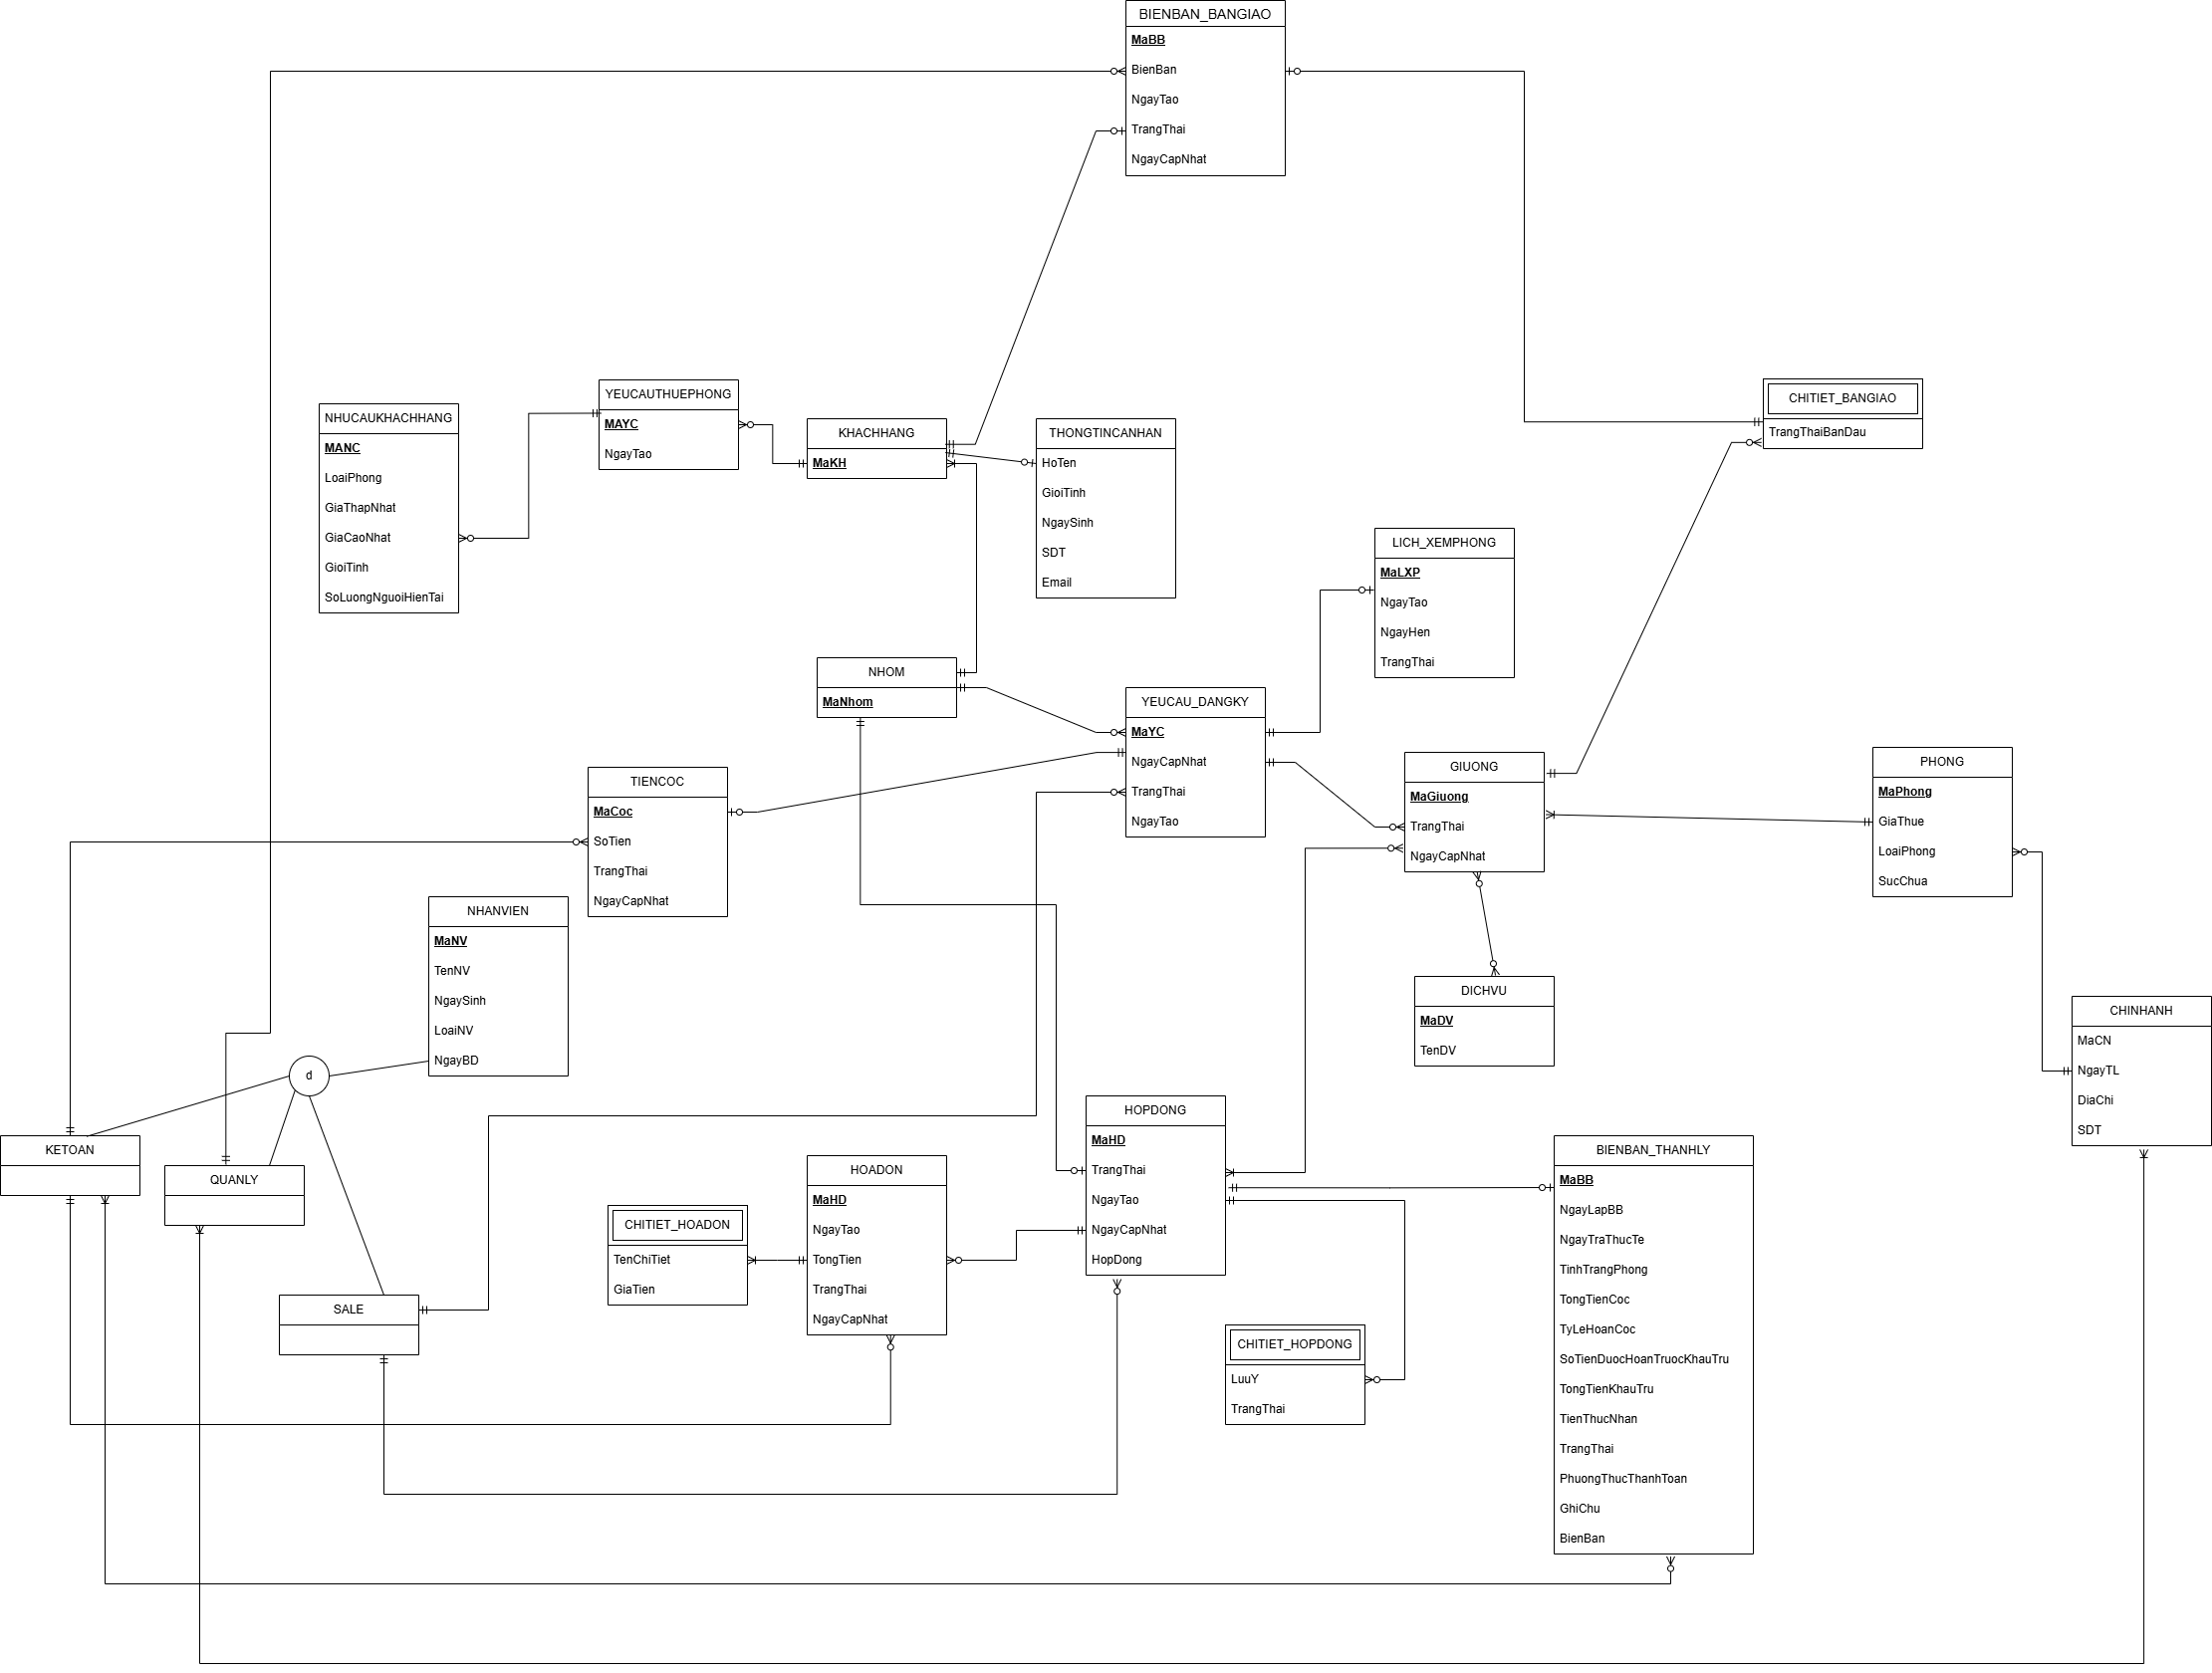
\includegraphics[width=0.98\textwidth]{images/ERD.drawio(1).png}
    \caption{Mô hình ERD của hệ thống HomeStay Dorm}
\end{figure}


\newpage
\section{System Use-case Diagram}

\begin{figure}[H]
    \centering
    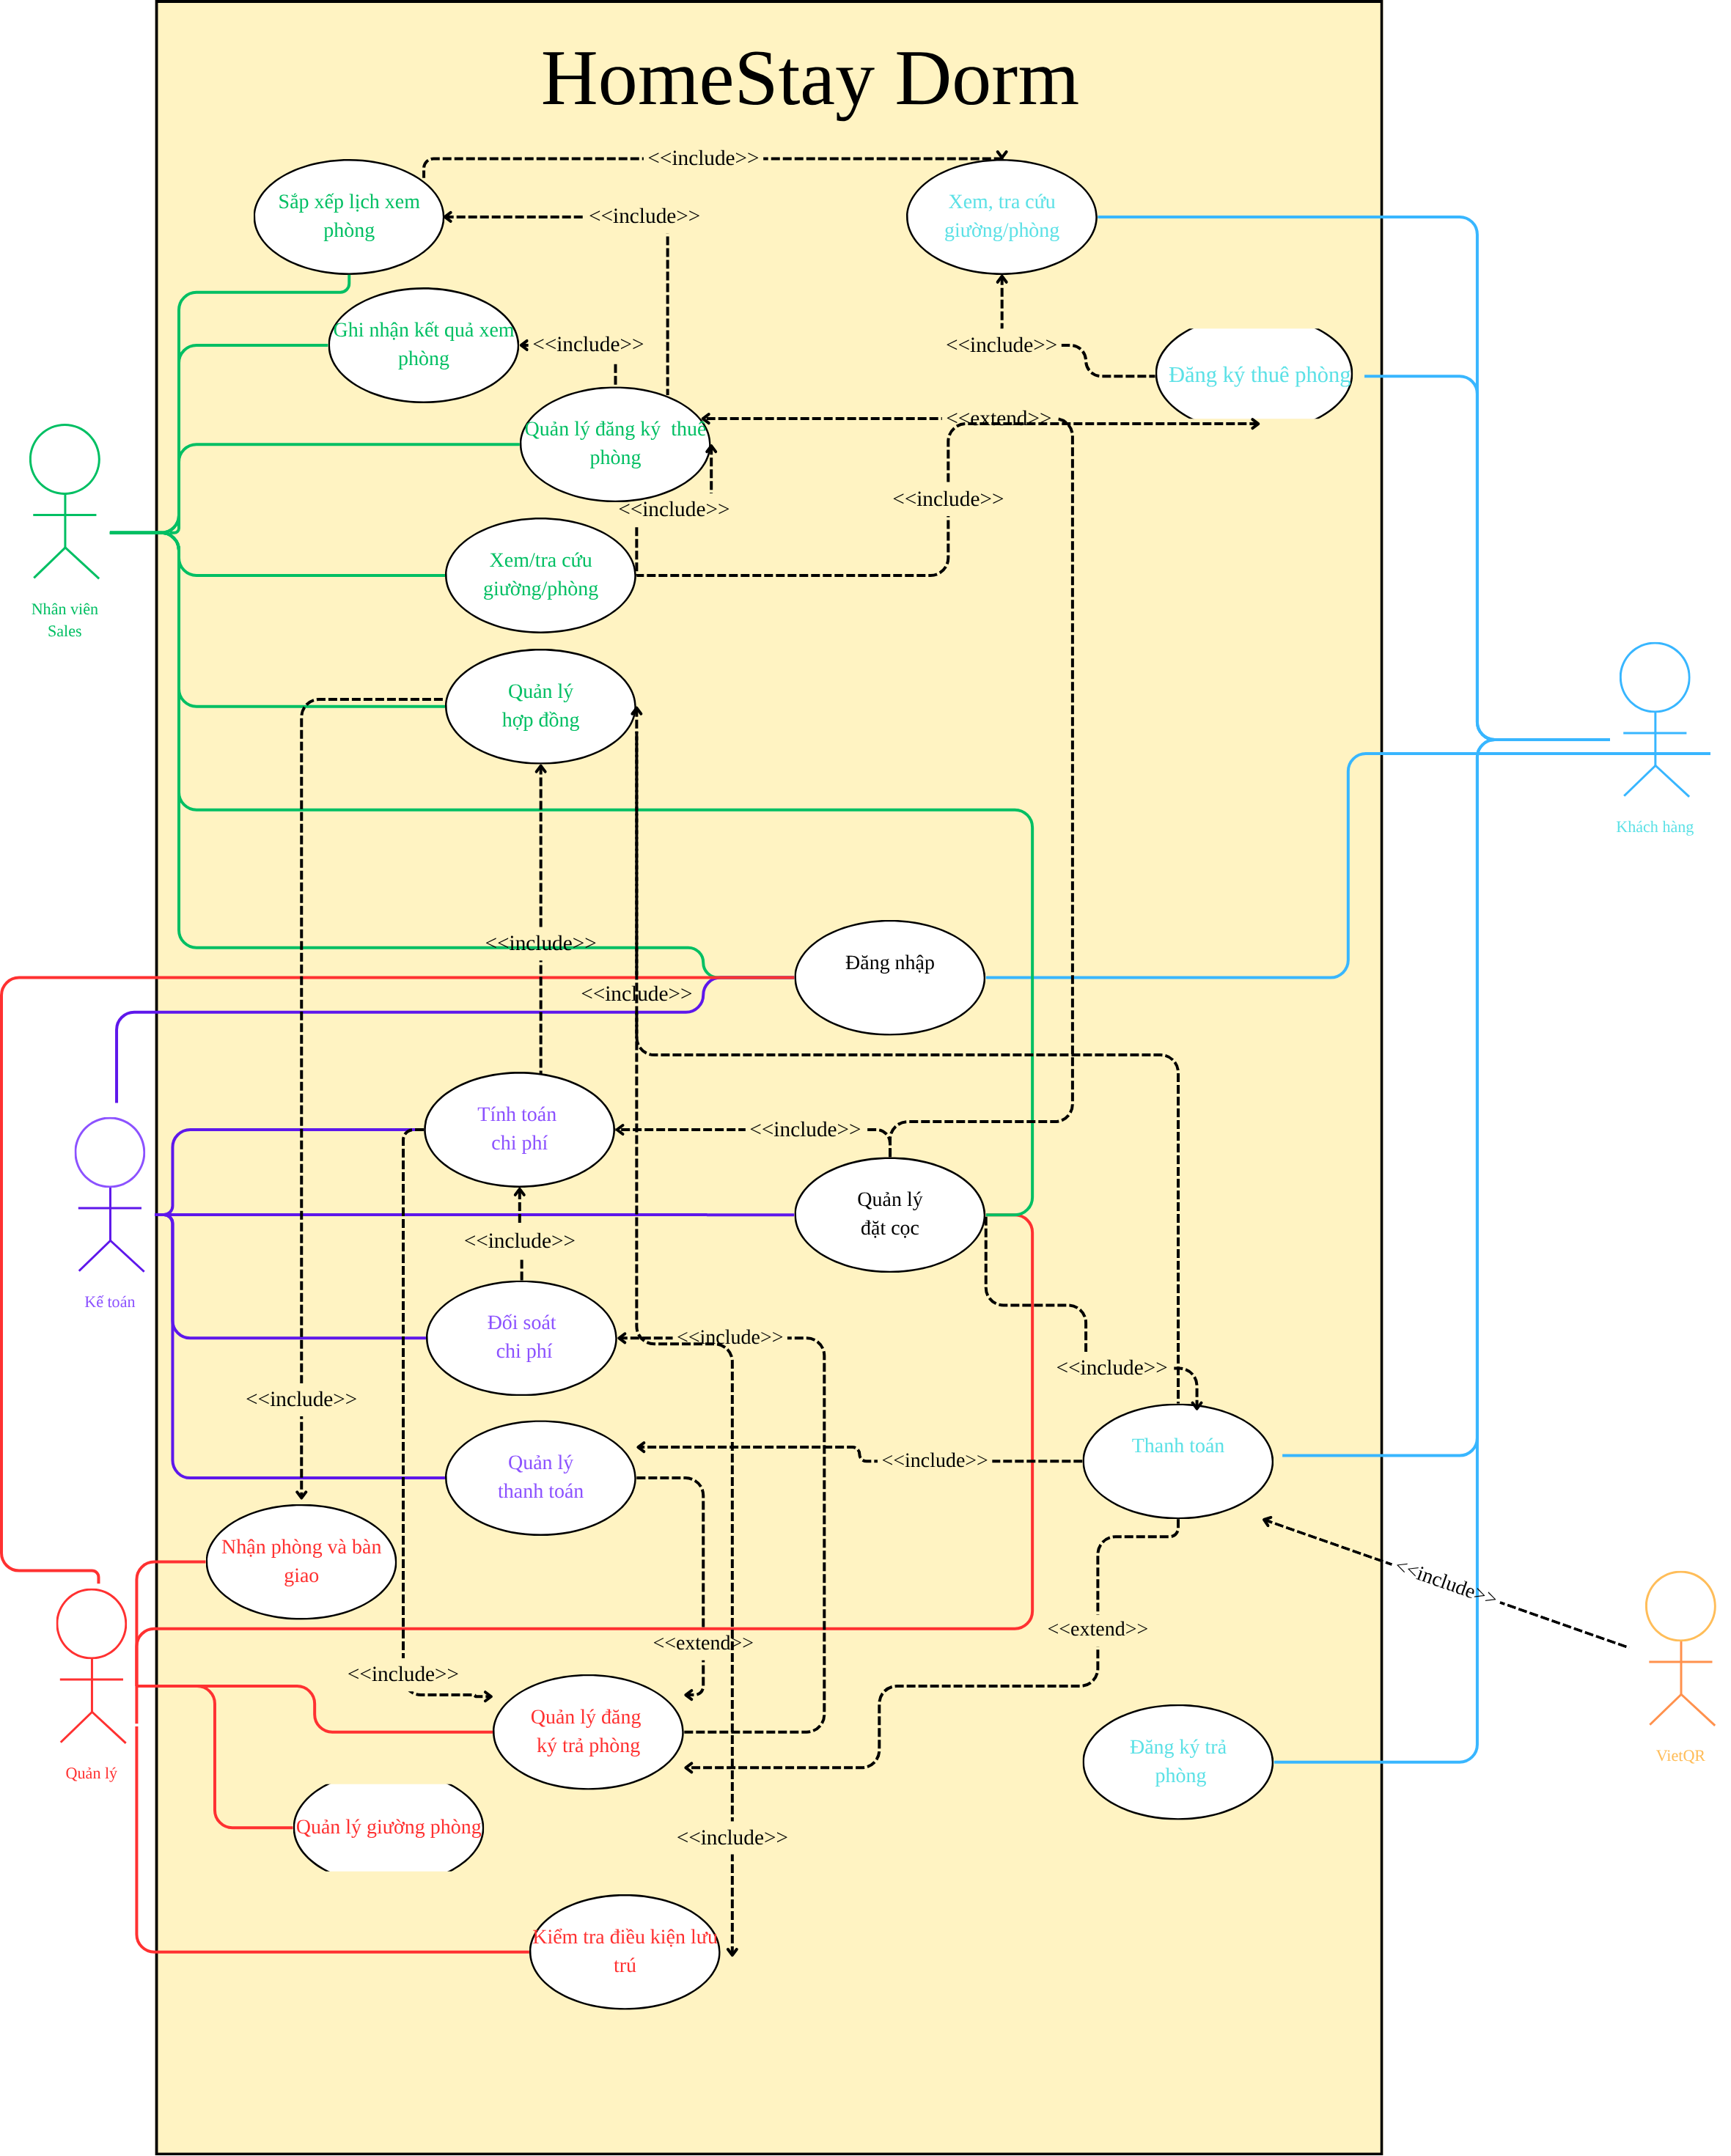
\includegraphics[width=0.98\textwidth]{images/SystemUseCase.png}
    \caption{Mô hình Use-case hệ thống}
\end{figure}
\newpage


\subsection{Đặc tả System Use Case}
% ============================================================
% SUC1
% ============================================================
\begin{table}[H]
\centering
\begin{tabularx}{\textwidth}{|>{\centering\arraybackslash\bfseries}m{3.5cm}|X|}
    \hline
    Use Case & {\centering\textbf{SUC1: Đăng nhập}\par} \\
    \hline
    Mô tả & Cho phép người dùng truy cập hệ thống để thực hiện các chức năng tương ứng với vai trò. \\
    \hline
    Actor &
    \vspace{0.3cm}
    \begin{itemize}
        \item Nhân viên Sales
        \item Kế toán
        \item Quản lý
        \item Khách hàng 
    \end{itemize} \\
    \hline
    Sự kiện kích hoạt & Người dùng chọn chức năng ``Đăng nhập''. \\
    \hline
    Tiền điều kiện & Người dùng đã có tài khoản. \\
    \hline
    Hậu điều kiện & Người dùng đăng nhập thành công vào hệ thống. \\
    \hline
    Dòng chính &
    \begin{enumerate}[leftmargin=*, nosep]
        \vspace{0.1cm}
        \item Hệ thống hiển thị màn hình đăng nhập.
        \item Người dùng nhập username và password.
        \item Hệ thống kiểm tra thông tin.
        \item Hệ thống xác thực thành công.
        \item Hệ thống chuyển vào màn hình chính.
        \item Kết thúc use case.
    \end{enumerate} \\
    \hline
    Dòng thay thế &
    \begin{itemize}[leftmargin=*, nosep, label=-]
        \vspace{0.1cm}
        \item \textbf{A1 -- Sai thông tin đăng nhập:} Hệ thống hiển thị lỗi; người dùng nhập lại.
        \item \textbf{A2 -- Quên mật khẩu:} Hệ thống hiển thị form nhập email; người dùng nhập email; hệ thống gửi link reset.
    \end{itemize} \\
    \hline
    Use-Case liên quan & Không. \\
    \hline
\end{tabularx}
\caption{Đặc tả SUC1: Đăng nhập}
\end{table}


\vspace{1cm}

% ============================================================
% SUC2
% ============================================================
\begin{table}[H]
\centering
\begin{tabularx}{\textwidth}{|>{\centering\arraybackslash\bfseries}m{3.5cm}|X|}
    \hline
    Use Case & {\centering\textbf{SUC2: Đăng ký thuê phòng}\par} \\
    \hline
    Mô tả & Khách hàng gửi yêu cầu thuê phòng tới hệ thống. \\
    \hline
    Actor &
    \begin{itemize}[leftmargin=*, nosep, label=\textbullet]
        \vspace{0.1cm}
        \item Khách hàng
    \end{itemize} \\
    \hline
    Sự kiện kích hoạt & Khách hàng chọn ``Đăng ký thuê phòng''. \\
    \hline
    Tiền điều kiện & Khách hàng đã đăng nhập. \\
    \hline
    Hậu điều kiện & Yêu cầu thuê được tạo. \\
    \hline
    Dòng chính &
    \begin{enumerate}[leftmargin=*, nosep]
        \vspace{0.1cm}
        \item Hệ thống hiển thị danh sách phòng.
        \item Khách hàng tra cứu phòng.
        \item Khách hàng chọn phòng.
        \item Khách hàng nhập thông tin thuê.
        \item Hệ thống lưu yêu cầu thuê.
        \item Kết thúc.
    \end{enumerate} \\
    \hline
    Dòng thay thế &
    \begin{itemize}[leftmargin=*, nosep, label=-]
        \vspace{0.1cm}
        \item \textbf{A1 -- Không có phòng phù hợp:} Hệ thống thông báo; kết thúc.
    \end{itemize} \\
    \hline
    Use-Case liên quan &
    \begin{itemize}[leftmargin=*, nosep, label=-]
        \vspace{0.1cm}
        \item \textit{(include)} Xem/tra cứu giường/phòng.
    \end{itemize} \\
    \hline
\end{tabularx}
\caption{Đặc tả SUC2: Đăng ký thuê phòng}
\end{table}


\vspace{1cm}

% ============================================================
% SUC3
% ============================================================
\begin{table}[H]
\centering
\begin{tabularx}{\textwidth}{|>{\centering\arraybackslash\bfseries}m{3.5cm}|X|}
    \hline
    Use Case & {\centering\textbf{SUC3: Quản lý đăng ký thuê phòng}\par} \\
    \hline
    Mô tả & Nhân viên Sales tiếp nhận yêu cầu thuê, tra cứu phòng phù hợp, sắp xếp lịch xem phòng và ghi nhận kết quả xem phòng của khách hàng. \\
    \hline
    Actor &
    \begin{itemize}[leftmargin=*, nosep, label=\textbullet]
        \vspace{0.1cm}
        \item Nhân viên Sales
    \end{itemize} \\
    \hline
    Sự kiện kích hoạt & Có yêu cầu thuê phòng từ khách hàng. \\
    \hline
    Tiền điều kiện & Nhân viên đã đăng nhập và có yêu cầu thuê. \\
    \hline
    Hậu điều kiện & Yêu cầu thuê được cập nhật trạng thái sau xem phòng; nếu khách đồng ý thuê thì sẵn sàng chuyển sang xử lý đặt cọc. \\
    \hline
    Dòng chính &
    \begin{enumerate}[leftmargin=*, nosep]
        \vspace{0.1cm}
        \item Hệ thống hiển thị danh sách yêu cầu thuê.
        \item Nhân viên chọn yêu cầu.
        \item Thực hiện \textbf{SUC13} để tra cứu phòng/giường phù hợp.
        \item Thực hiện \textbf{SUC14} để sắp xếp lịch xem phòng với khách hàng.
        \item Đến lịch hẹn, thực hiện \textbf{SUC15} để ghi nhận kết quả xem phòng.
        \item Nếu khách hàng đồng ý thuê, nhân viên xác nhận nhu cầu thuê trên hệ thống.
        \item Hệ thống cập nhật trạng thái yêu cầu và tạo cơ sở để thực hiện \textbf{SUC4}.
        \item Kết thúc.
    \end{enumerate} \\
    \hline
    Dòng thay thế &
    \begin{itemize}[leftmargin=*, nosep, label=-]
        \vspace{0.1cm}
        \item \textbf{A1 -- Không còn phòng phù hợp:} Hệ thống thông báo; nhân viên tư vấn lại phòng/giường khác hoặc kết thúc yêu cầu.
        \item \textbf{A2 -- Khách không tham gia hoặc không đồng ý sau khi xem phòng:} Nhân viên ghi nhận kết quả; hệ thống cập nhật trạng thái yêu cầu là chưa tiếp tục thuê.
    \end{itemize} \\
    \hline
    Use-Case liên quan &
    \begin{itemize}[leftmargin=*, nosep, label=-]
        \vspace{0.1cm}
        \item \textit{(include)} Xem/tra cứu giường/phòng.
        \item \textit{(include)} Sắp xếp lịch xem phòng.
        \item \textit{(include)} Ghi nhận kết quả xem phòng.
        \item \textit{(extend)} Quản lý đặt cọc.
\end{itemize} \\
    \hline
\end{tabularx}
\caption{Đặc tả SUC3: Quản lý đăng ký thuê phòng}
\end{table}



\vspace{1cm}

% ============================================================
% SUC4
% ============================================================
\begin{table}[H]
\centering
\begin{tabularx}{\textwidth}{|>{\centering\arraybackslash\bfseries}m{3.5cm}|X|}
    \hline
    Use Case & {\centering\textbf{SUC4: Quản lý đặt cọc}\par} \\
    \hline
    Mô tả & Thực hiện tạo và xử lý yêu cầu đặt cọc cho việc thuê phòng. \\
    \hline
    Actor &
    \begin{itemize}[leftmargin=*, nosep, label=\textbullet]
        \vspace{0.1cm}
        \item Nhân viên Sales
        \item Kế toán
        \item Quản lý
    \end{itemize} \\
    \hline
    Sự kiện kích hoạt & Yêu cầu thuê phòng được chấp nhận. \\
    \hline
    Tiền điều kiện & Yêu cầu thuê đã được xác nhận và người dùng đã đăng nhập hợp lệ. \\
    \hline
    Hậu điều kiện & Đặt cọc được ghi nhận thành công. \\
    \hline
    Dòng chính &
    \begin{enumerate}[leftmargin=*, nosep]
        \vspace{0.1cm}
        \item Nhân viên tạo yêu cầu đặt cọc.
        \item Hệ thống hiển thị thông tin đặt cọc.
        \item Kế toán kiểm tra và nhập số tiền cọc.
        \item Hệ thống xác nhận số tiền.
        \item Thực hiện thanh toán.
        \item Hệ thống lưu trạng thái đặt cọc.
        \item Kết thúc.
    \end{enumerate} \\
    \hline
    Dòng thay thế &
    \begin{itemize}[leftmargin=*, nosep, label=-]
        \vspace{0.1cm}
        \item \textbf{A1 -- Thanh toán thất bại:} Hệ thống thông báo lỗi; cho phép thực hiện lại.
    \end{itemize} \\
    \hline
    Use-Case liên quan &
    \begin{itemize}[leftmargin=*, nosep, label=-]
        \vspace{0.1cm}
        \item \textit{(include)} Thanh toán.
        \item \textit{(include)} Tính toán chi phí.
\end{itemize} \\
    \hline
\end{tabularx}
\caption{Đặc tả SUC4: Quản lý đặt cọc}
\end{table}


\vspace{1cm}

% ============================================================
% SUC5
% ============================================================
\begin{table}[H]
\centering
\begin{tabularx}{\textwidth}{|>{\centering\arraybackslash\bfseries}m{3.5cm}|X|}
    \hline
    Use Case & {\centering\textbf{SUC5: Thanh toán}\par} \\
    \hline
    Mô tả & Thực hiện giao dịch thanh toán cho các nghiệp vụ trong hệ thống. \\
    \hline
    Actor &
    \begin{itemize}[leftmargin=*, nosep, label=\textbullet]
        \vspace{0.1cm}
        \item Khách hàng
        \item VietQR
    \end{itemize} \\
    \hline
    Sự kiện kích hoạt & Có yêu cầu thanh toán từ hệ thống. \\
    \hline
    Tiền điều kiện & Có giao dịch cần thanh toán. \\
    \hline
    Hậu điều kiện & Giao dịch thanh toán thành công hoặc thất bại được ghi nhận. \\
    \hline
    Dòng chính &
    \begin{enumerate}[leftmargin=*, nosep]
        \vspace{0.1cm}
        \item Hệ thống hiển thị thông tin thanh toán.
        \item Khách hàng chọn phương thức thanh toán.
        \item Hệ thống gửi yêu cầu tới VietQR.
        \item VietQR xử lý giao dịch.
        \item Hệ thống nhận kết quả.
        \item Hệ thống cập nhật trạng thái thanh toán.
        \item Kết thúc.
    \end{enumerate} \\
    \hline
    Dòng thay thế &
    \begin{itemize}[leftmargin=*, nosep, label=-]
        \vspace{0.1cm}
        \item \textbf{A1 -- Thanh toán thất bại:} Hệ thống hiển thị lỗi; cho phép thanh toán lại.
        \item \textbf{A2 -- Timeout / lỗi kết nối VietQR:} Hệ thống thông báo lỗi; giao dịch bị hủy.
    \end{itemize} \\
    \hline
    Use-Case liên quan &
    \begin{itemize}[leftmargin=*, nosep, label=-]
        \vspace{0.1cm}
        \item \textit{(include)} Quản lý thanh toán.
\end{itemize} \\
    \hline
\end{tabularx}
\caption{Đặc tả SUC5: Thanh toán}
\end{table}



\vspace{1cm}

% ============================================================
% SUC6
% ============================================================
\begin{table}[H]
\centering
\begin{tabularx}{\textwidth}{|>{\centering\arraybackslash\bfseries}m{3.5cm}|X|}
    \hline
    Use Case & {\centering\textbf{SUC6: Quản lý thanh toán}\par} \\
    \hline
    Mô tả & Quản lý và xử lý các giao dịch thanh toán trong hệ thống. \\
    \hline
    Actor &
    \begin{itemize}[leftmargin=*, nosep, label=\textbullet]
        \vspace{0.1cm}
        \item Kế toán
    \end{itemize} \\
    \hline
    Sự kiện kích hoạt & Có giao dịch thanh toán phát sinh. \\
    \hline
    Tiền điều kiện & Có dữ liệu giao dịch. \\
    \hline
    Hậu điều kiện & Giao dịch được ghi nhận và xử lý. \\
    \hline
    Dòng chính &
    \begin{enumerate}[leftmargin=*, nosep]
        \vspace{0.1cm}
        \item Hệ thống nhận thông tin giao dịch.
        \item Kế toán kiểm tra giao dịch.
        \item Hệ thống đối chiếu thông tin.
        \item Kế toán xác nhận giao dịch.
        \item Hệ thống lưu vào hệ thống.
        \item Kết thúc.
    \end{enumerate} \\
    \hline
    Dòng thay thế &
    \begin{itemize}[leftmargin=*, nosep, label=-]
        \vspace{0.1cm}
        \item \textbf{A1 -- Sai lệch giao dịch:} Hệ thống thông báo lỗi; kế toán kiểm tra lại.
        \item \textbf{A2 -- Giao dịch bị hủy:} Hệ thống cập nhật trạng thái hủy.
    \end{itemize} \\
    \hline
    Use-Case liên quan &
    \begin{itemize}[leftmargin=*, nosep, label=-]
        \vspace{0.1cm}
        \item \textit{(được include bởi)} Thanh toán.
\end{itemize} \\
    \hline
\end{tabularx}
\caption{Đặc tả SUC6: Quản lý thanh toán}
\end{table}

\vspace{1cm}

% ============================================================
% SUC7
% ============================================================
\begin{table}[H]
\centering
\begin{tabularx}{\textwidth}{|>{\centering\arraybackslash\bfseries}m{3.5cm}|X|}
    \hline
    Use Case & {\centering\textbf{SUC7: Quản lý hợp đồng}\par} \\
    \hline
    Mô tả & Lập, xác nhận và lưu hợp đồng thuê phòng sau khi khách hàng đã đặt cọc và đủ điều kiện lưu trú; đồng thời chuyển thông tin cho bước nhận phòng/bàn giao. \\
    \hline
    Actor &
    \begin{itemize}[leftmargin=*, nosep, label=\textbullet]
        \vspace{0.1cm}
        \item Nhân viên Sales
    \end{itemize} \\
    \hline
    Sự kiện kích hoạt & Khách hàng hoàn tất đặt cọc và đủ điều kiện thuê. \\
    \hline
    Tiền điều kiện & Khách hàng đã đặt cọc, đã được kiểm tra điều kiện lưu trú và nhân viên Sales đã đăng nhập. \\
    \hline
    Hậu điều kiện & Hợp đồng được tạo, lưu trong hệ thống và sẵn sàng cho bước nhận phòng/bàn giao. \\
    \hline
    Dòng chính &
    \begin{enumerate}[leftmargin=*, nosep]
        \vspace{0.1cm}
        \item Nhân viên chọn tạo hợp đồng.
        \item Hệ thống hiển thị thông tin khách hàng, phòng/giường, trạng thái đặt cọc và hồ sơ lưu trú.
        \item Thực hiện \textbf{SUC16} để kiểm tra điều kiện lưu trú trước khi lập hợp đồng.
        \item Thực hiện \textbf{SUC9} để tính các khoản chi phí cần thu khi ký hợp đồng.
        \item Nhân viên nhập các thông tin hợp đồng.
        \item Thực hiện \textbf{SUC5} nếu cần thu thêm tiền khi ký hợp đồng.
        \item Hệ thống sinh mã hợp đồng và lưu hợp đồng.
        \item Hệ thống chuyển thông tin cho quản lý để thực hiện \textbf{SUC17}.
        \item Kết thúc.
    \end{enumerate} \\
    \hline
    Dòng thay thế &
    \begin{itemize}[leftmargin=*, nosep, label=-]
        \vspace{0.1cm}
        \item \textbf{A1 -- Thông tin hợp đồng không hợp lệ:} Hệ thống thông báo lỗi; nhân viên nhập lại.
        \item \textbf{A2 -- Khách hàng không đủ điều kiện lưu trú:} Hệ thống không cho phép lập hợp đồng; ghi nhận kết quả kiểm tra và kết thúc.
        \item \textbf{A3 -- Thanh toán khi ký hợp đồng không thành công:} Hệ thống thông báo lỗi; hợp đồng chưa được kích hoạt.
    \end{itemize} \\
    \hline
    Use-Case liên quan &
    \begin{itemize}[leftmargin=*, nosep, label=-]
        \vspace{0.1cm}
        \item \textit{(include)} Kiểm tra điều kiện lưu trú.
        \item \textit{(include)} Tính toán chi phí.
        \item \textit{(include)} Thanh toán.
        \item \textit{(include)} Nhận phòng và bàn giao.
\end{itemize} \\
    \hline
\end{tabularx}
\caption{Đặc tả SUC7: Quản lý hợp đồng}
\end{table}



\vspace{1cm}

% ============================================================
% SUC8
% ============================================================
\begin{table}[H]
\centering
\begin{tabularx}{\textwidth}{|>{\centering\arraybackslash\bfseries}m{3.5cm}|X|}
    \hline
    Use Case & {\centering\textbf{SUC8: Đối soát chi phí}\par} \\
    \hline
    Mô tả & Thực hiện đối soát chi phí khi khách trả phòng, tổng hợp số tiền khách phải thanh toán thêm hoặc được hoàn lại dựa trên kết quả tính toán chi phí. \\
    \hline
    Actor &
    \begin{itemize}[leftmargin=*, nosep, label=\textbullet]
        \vspace{0.1cm}
        \item Kế toán
    \end{itemize} \\
    \hline
    Sự kiện kích hoạt & Có yêu cầu trả phòng. \\
    \hline
    Tiền điều kiện & Có dữ liệu thuê phòng và người dùng đã đăng nhập. \\
    \hline
    Hậu điều kiện & Kết quả đối soát chi phí được xác định và lưu để phục vụ quyết toán trả phòng. \\
    \hline
    Dòng chính &
    \begin{enumerate}[leftmargin=*, nosep]
        \vspace{0.1cm}
        \item Hệ thống hiển thị thông tin thuê.
        \item Kế toán kiểm tra thời gian thuê, tình trạng phòng và thông tin đặt cọc.
        \item Thực hiện \textbf{SUC9} để tính các khoản chi phí liên quan.
        \item Hệ thống tổng hợp các khoản phải thu thêm hoặc phải hoàn lại cho khách hàng.
        \item Kế toán xác nhận kết quả đối soát.
        \item Hệ thống lưu kết quả đối soát.
        \item Kết thúc.
    \end{enumerate} \\
    \hline
    Dòng thay thế &
    \begin{itemize}[leftmargin=*, nosep, label=-]
        \vspace{0.1cm}
        \item \textbf{A1 -- Thiếu dữ liệu:} Hệ thống thông báo lỗi; không thực hiện tiếp.
        \item \textbf{A2 -- Dữ liệu bàn giao chưa đầy đủ:} Hệ thống tạm dừng đối soát; yêu cầu cập nhật lại tình trạng phòng/tài sản.
    \end{itemize} \\
    \hline
    Use-Case liên quan &
    \begin{itemize}[leftmargin=*, nosep, label=-]
        \vspace{0.1cm}
        \item \textit{(include)} Tính toán chi phí.
        \item \textit{(include)} trong Quản lý đăng ký trả phòng.
\end{itemize} \\
    \hline
\end{tabularx}
\caption{Đặc tả SUC8: Đối soát chi phí}
\end{table}

\vspace{1cm}

% ============================================================
% SUC9
% ============================================================
\begin{table}[H]
\centering
\begin{tabularx}{\textwidth}{|>{\centering\arraybackslash\bfseries}m{3.5cm}|X|}
    \hline
    Use Case & {\centering\textbf{SUC9: Tính toán chi phí}\par} \\
    \hline
    Mô tả & Thực hiện tính toán các khoản chi phí liên quan đến thuê phòng, bao gồm tiền cọc, tiền thuê và các chi phí phát sinh. \\
    \hline
    Actor &
    \begin{itemize}[leftmargin=*, nosep, label=\textbullet]
        \vspace{0.1cm}
        \item Kế toán
    \end{itemize} \\
    \hline
    Sự kiện kích hoạt & Có yêu cầu xác định chi phí từ hệ thống (đặt cọc, lập hợp đồng hoặc trả phòng). \\
    \hline
    Tiền điều kiện & Có dữ liệu liên quan đến thuê phòng (giá phòng, thời gian thuê, thông tin khách hàng) và người dùng đã đăng nhập. \\
    \hline
    Hậu điều kiện & Các khoản chi phí được tính toán và cung cấp cho use case gọi. \\
    \hline
    Dòng chính &
    \begin{enumerate}[leftmargin=*, nosep]
        \vspace{0.1cm}
        \item Hệ thống nhận yêu cầu tính toán chi phí.
        \item Hệ thống xác định loại nghiệp vụ (đặt cọc / hợp đồng / trả phòng).
        \item Hệ thống truy xuất dữ liệu liên quan.
        \item Hệ thống tính toán chi phí theo nghiệp vụ:
        \begin{itemize}[leftmargin=*, nosep, label=\textbullet]
            \item Tiền cọc (nếu đặt cọc).
            \item Tiền thuê (nếu lập hợp đồng).
            \item Chi phí phát sinh (nếu trả phòng).
        \end{itemize}
        \item Hệ thống tổng hợp kết quả.
        \item Hệ thống trả kết quả cho use case gọi.
        \item Kết thúc.
    \end{enumerate} \\
    \hline
    Dòng thay thế &
    \begin{itemize}[leftmargin=*, nosep, label=-]
        \vspace{0.1cm}
        \item \textbf{A1 -- Thiếu dữ liệu:} Hệ thống phát hiện thiếu thông tin (giá phòng / thời gian thuê / hợp đồng); hệ thống thông báo lỗi; không thực hiện tính toán.
        \item \textbf{A2 -- Dữ liệu không hợp lệ:} Hệ thống phát hiện dữ liệu sai (thời gian âm, giá không hợp lệ); hệ thống yêu cầu kiểm tra lại; kết thúc.
        \item \textbf{A3 -- Không có chi phí phát sinh:} Hệ thống xác định không có khoản phụ phí; hệ thống trả kết quả chỉ gồm chi phí cơ bản.
    \end{itemize} \\
    \hline
    Use-Case liên quan &
    \begin{itemize}[leftmargin=*, nosep, label=-]
        \vspace{0.1cm}
        \item \textit{(được include bởi)} Quản lý đăng ký trả phòng.
        \item \textit{(được include bởi)} Quản lý đặt cọc.
        \item \textit{(được include bởi)} Quản lý hợp đồng.
\end{itemize} \\
    \hline
\end{tabularx}
\caption{Đặc tả SUC9: Tính toán chi phí}
\end{table}


\vspace{1cm}

% ============================================================
% SUC10
% ============================================================
\begin{table}[H]
\centering
\begin{tabularx}{\textwidth}{|>{\centering\arraybackslash\bfseries}m{3.5cm}|X|}
    \hline
    Use Case & {\centering\textbf{SUC10: Đăng ký trả phòng}\par} \\
    \hline
    Mô tả & Khách hàng gửi yêu cầu trả phòng tới hệ thống. \\
    \hline
    Actor &
    \begin{itemize}[leftmargin=*, nosep, label=\textbullet]
        \vspace{0.1cm}
        \item Khách hàng
    \end{itemize} \\
    \hline
    Sự kiện kích hoạt & Khách hàng chọn chức năng ``Đăng ký trả phòng''. \\
    \hline
    Tiền điều kiện & Khách hàng đang có hợp đồng thuê và đã đăng nhập. \\
    \hline
    Hậu điều kiện & Yêu cầu trả phòng được tạo. \\
    \hline
    Dòng chính &
    \begin{enumerate}[leftmargin=*, nosep]
        \vspace{0.1cm}
        \item Hệ thống hiển thị thông tin thuê.
        \item Khách hàng chọn trả phòng.
        \item Khách hàng xác nhận.
        \item Hệ thống tạo yêu cầu trả phòng.
        \item Kết thúc.
    \end{enumerate} \\
    \hline
    Dòng thay thế &
    \begin{itemize}[leftmargin=*, nosep, label=-]
        \vspace{0.1cm}
        \item \textbf{A1 -- Không có hợp đồng thuê:} Hệ thống thông báo; kết thúc.
    \end{itemize} \\
    \hline
    Use-Case liên quan & Không. \\
    \hline
\end{tabularx}
\caption{Đặc tả SUC10: Đăng ký trả phòng}
\end{table}



\vspace{1cm}

% ============================================================
% SUC11
% ============================================================
\begin{table}[H]
\centering
\begin{tabularx}{\textwidth}{|>{\centering\arraybackslash\bfseries}m{3.5cm}|X|}
    \hline
    Use Case & {\centering\textbf{SUC11: Quản lý đăng ký trả phòng}\par} \\
    \hline
    Mô tả & Tiếp nhận và xử lý yêu cầu trả phòng của khách hàng, bao gồm đối soát chi phí, quyết toán thanh toán/hoàn cọc, thanh lý hợp đồng và cập nhật kết thúc lưu trú. \\
    \hline
    Actor &
    \begin{itemize}[leftmargin=*, nosep, label=\textbullet]
        \vspace{0.1cm}
        \item Quản lý
    \end{itemize} \\
    \hline
    Sự kiện kích hoạt & Có yêu cầu trả phòng từ khách hàng. \\
    \hline
    Tiền điều kiện &
    \begin{itemize}[leftmargin=*, nosep, label=\textbullet]
        \vspace{0.1cm}
        \item Có yêu cầu trả phòng.
        \item Quản lý đã đăng nhập.
    \end{itemize} \\
    \hline
    Hậu điều kiện & Trả phòng được xử lý hoàn tất; hợp đồng được thanh lý và trạng thái phòng/giường được cập nhật. \\
    \hline
    Dòng chính &
    \begin{enumerate}[leftmargin=*, nosep]
        \vspace{0.1cm}
        \item Hệ thống hiển thị danh sách yêu cầu trả phòng.
        \item Quản lý chọn yêu cầu.
        \item Hệ thống hiển thị thông tin thuê, hợp đồng, tiền cọc và tình trạng phòng hiện tại.
        \item Thực hiện \textbf{SUC8} để đối soát chi phí trả phòng.
        \item Hệ thống hiển thị kết quả đối soát, bao gồm số tiền cần thu thêm hoặc số tiền cần hoàn lại.
        \item Nếu có phát sinh thanh toán/hoàn tiền, thực hiện \textbf{SUC5}.
        \item Quản lý ký xác nhận biên bản trả phòng và thanh lý hợp đồng với khách hàng.
        \item Quản lý ghi nhận việc thu hồi chìa khóa/thẻ ra vào và cập nhật bàn giao tài sản.
        \item Hệ thống cập nhật trạng thái hợp đồng là đã thanh lý và trạng thái phòng/giường là trống.
        \item Hệ thống thông báo hoàn tất trả phòng.
        \item Kết thúc.
    \end{enumerate} \\
    \hline
    Dòng thay thế &
    \begin{itemize}[leftmargin=*, nosep, label=-]
        \vspace{0.1cm}
        \item \textbf{A1 -- Thanh toán/hoàn tiền chưa hoàn tất:} Hệ thống giữ trạng thái xử lý trả phòng; chưa cho phép thanh lý hợp đồng.
        \item \textbf{A2 -- Khách chưa bàn giao đủ chìa khóa, thẻ ra vào hoặc tài sản:} Quản lý ghi nhận thiếu sót; yêu cầu khách hoàn tất bàn giao trước khi tiếp tục.
        \item \textbf{A3 -- Lỗi cập nhật trạng thái hợp đồng hoặc phòng:} Hệ thống thông báo lỗi; trả phòng chưa được hoàn tất.
    \end{itemize} \\
    \hline
    Use-Case liên quan &
    \begin{itemize}[leftmargin=*, nosep, label=-]
        \vspace{0.1cm}
        \item \textit{(include)} Đối soát chi phí.
        \item \textit{(extend)} Thanh toán.
\end{itemize} \\
    \hline
\end{tabularx}
\caption{Đặc tả SUC11: Quản lý đăng ký trả phòng}
\end{table}


\vspace{1cm}

% ============================================================
% SUC12
% ============================================================
\begin{table}[H]
\centering
\begin{tabularx}{\textwidth}{|>{\centering\arraybackslash\bfseries}m{3.5cm}|X|}
    \hline
    Use Case & {\centering\textbf{SUC12: Quản lý giường phòng}\par} \\
    \hline
    Mô tả & Quản lý thông tin giường/phòng (thêm, sửa, xóa, xem). \\
    \hline
    Actor &
    \begin{itemize}[leftmargin=*, nosep, label=\textbullet]
        \vspace{0.1cm}
        \item Quản lý
    \end{itemize} \\
    \hline
    Sự kiện kích hoạt & Quản lý chọn chức năng quản lý giường/phòng. \\
    \hline
    Tiền điều kiện & Quản lý đã đăng nhập. \\
    \hline
    Hậu điều kiện & Thông tin giường/phòng được cập nhật. \\
    \hline
    Dòng chính &
    \begin{enumerate}[leftmargin=*, nosep]
        \vspace{0.1cm}
        \item Hệ thống hiển thị danh sách giường/phòng.
        \item Quản lý chọn thao tác: thêm / sửa / xóa / xem.
        \item Quản lý chọn thông tin để xem / nhập thông tin mới / chỉnh sửa thông tin đã có / xóa thông tin cũ.
        \item Hệ thống mở dữ liệu xem / lưu dữ liệu mới / cập nhật dữ liệu tương ứng / xóa dữ liệu.
        \item Kết thúc.
    \end{enumerate} \\
    \hline
    Dòng thay thế &
    \begin{itemize}[leftmargin=*, nosep, label=-]
        \vspace{0.1cm}
        \item \textbf{A1 -- Dữ liệu không hợp lệ:} Hệ thống thông báo lỗi; nhập lại.
        \item \textbf{A2 -- Không thể xóa (đang được sử dụng):} Hệ thống từ chối; kết thúc.
    \end{itemize} \\
    \hline
    Use-Case liên quan & Không. \\
    \hline
\end{tabularx}
\caption{Đặc tả SUC12: Quản lý giường phòng}
\end{table}


\vspace{1cm}

% ============================================================
% SUC13
% ============================================================
\begin{table}[H]
\centering
\begin{tabularx}{\textwidth}{|>{\centering\arraybackslash\bfseries}m{3.5cm}|X|}
    \hline
    Use Case & {\centering\textbf{SUC13: Xem/tra cứu giường/phòng}\par} \\
    \hline
    Mô tả & Cho phép người dùng tra cứu thông tin phòng/giường. \\
    \hline
    Actor &
    \begin{itemize}[leftmargin=*, nosep, label=\textbullet]
        \vspace{0.1cm}
        \item Nhân viên Sales
        \item Khách hàng
    \end{itemize} \\
    \hline
    Sự kiện kích hoạt & Người dùng chọn chức năng tra cứu. \\
    \hline
    Tiền điều kiện & Người dùng đã đăng nhập (có thể bỏ nếu hệ thống cho phép public). \\
    \hline
    Hậu điều kiện & Danh sách phòng được hiển thị. \\
    \hline
    Dòng chính &
    \begin{enumerate}[leftmargin=*, nosep]
        \vspace{0.1cm}
        \item Hệ thống hiển thị danh sách phòng.
        \item Người dùng nhập tiêu chí tìm kiếm.
        \item Hệ thống lọc dữ liệu.
        \item Hệ thống hiển thị kết quả.
        \item Người dùng xem chi tiết phòng.
        \item Kết thúc.
    \end{enumerate} \\
    \hline
    Dòng thay thế &
    \begin{itemize}[leftmargin=*, nosep, label=-]
        \vspace{0.1cm}
        \item \textbf{A1 -- Không có kết quả:} Hệ thống thông báo; cho phép tìm lại.
    \end{itemize} \\
    \hline
    Use-Case liên quan &
    \begin{itemize}[leftmargin=*, nosep, label=-]
        \vspace{0.1cm}
        \item \textit{(được include bởi)} Quản lý đăng ký thuê phòng.
        \item \textit{(được include bởi)} Đăng ký thuê phòng.
        \item \textit{(được include bởi)} Sắp xếp lịch xem phòng.
\end{itemize} \\
    \hline
\end{tabularx}
\caption{Đặc tả SUC13: Xem/tra cứu giường/phòng}
\end{table}

\vspace{1cm}

% ============================================================
% SUC14
% ============================================================
\begin{table}[H]
\centering
\begin{tabularx}{\textwidth}{|>{\centering\arraybackslash\bfseries}m{3.5cm}|X|}
    \hline
    Use Case & {\centering\textbf{SUC14: Sắp xếp lịch xem phòng}\par} \\
    \hline
    Mô tả & Nhân viên Sales sắp xếp lịch xem phòng với khách hàng và lưu lịch hẹn trên hệ thống. \\
    \hline
    Actor &
    \begin{itemize}[leftmargin=*, nosep, label=\textbullet]
        \vspace{0.1cm}
        \item Nhân viên Sales
    \end{itemize} \\
    \hline
    Sự kiện kích hoạt & Có yêu cầu thuê cần hẹn lịch xem phòng. \\
    \hline
    Tiền điều kiện & Yêu cầu thuê đang ở trạng thái xử lý và đã có phòng/giường phù hợp. \\
    \hline
    Hậu điều kiện & Lịch xem phòng được tạo và thông tin lịch hẹn được lưu trên hệ thống. \\
    \hline
    Dòng chính &
    \begin{enumerate}[leftmargin=*, nosep]
        \vspace{0.1cm}
        \item Nhân viên mở yêu cầu thuê cần sắp lịch xem phòng.
        \item Hệ thống hiển thị thông tin khách hàng, phòng/giường và các khung giờ khả dụng.
        \item Nhân viên trao đổi với khách hàng và chọn thời gian xem phòng phù hợp.
        \item Hệ thống ghi nhận lịch xem phòng.
        \item Hệ thống gửi hoặc hiển thị thông tin lịch hẹn cho khách hàng.
        \item Kết thúc.
    \end{enumerate} \\
    \hline
    Dòng thay thế &
    \begin{itemize}[leftmargin=*, nosep, label=-]
        \vspace{0.1cm}
        \item \textbf{A1 -- Không còn khung giờ phù hợp:} Hệ thống thông báo; nhân viên chọn thời gian khác hoặc tạm hoãn lịch.
        \item \textbf{A2 -- Khách hàng hủy lịch hẹn:} Hệ thống cập nhật trạng thái lịch là đã hủy; kết thúc.
    \end{itemize} \\
    \hline
    Use-Case liên quan &
    \begin{itemize}[leftmargin=*, nosep, label=-]
        \vspace{0.1cm}
        \item \textit{(include)} Xem/tra cứu giường/phòng.
        \item \textit{(được include bởi)} Quản lý đăng ký thuê phòng.
\end{itemize} \\
    \hline
\end{tabularx}
\caption{Đặc tả SUC14: Sắp xếp lịch xem phòng}
\end{table}



% ===================   =========================================
% SUC15
% ============================================================
\begin{table}[H]
\centering
\begin{tabularx}{\textwidth}{|>{\centering\arraybackslash\bfseries}m{3.5cm}|X|}
    \hline
    Use Case & {\centering\textbf{SUC15: Ghi nhận kết quả xem phòng}\par} \\
    \hline
    Mô tả & Nhân viên Sales ghi nhận kết quả buổi xem phòng và nhu cầu thuê của khách hàng sau khi xem thực tế. \\
    \hline
    Actor &
    \begin{itemize}[leftmargin=*, nosep, label=\textbullet]
        \vspace{0.1cm}
        \item Nhân viên Sales
    \end{itemize} \\
    \hline
    Sự kiện kích hoạt & Đến lịch xem phòng đã được tạo trước đó. \\
    \hline
    Tiền điều kiện & Đã có lịch xem phòng hợp lệ. \\
    \hline
    Hậu điều kiện & Kết quả xem phòng và nhu cầu tiếp tục thuê của khách hàng được lưu trên hệ thống. \\
    \hline
    Dòng chính &
    \begin{enumerate}[leftmargin=*, nosep]
        \vspace{0.1cm}
        \item Nhân viên mở lịch xem phòng cần xử lý.
        \item Hệ thống hiển thị thông tin lịch hẹn và phòng/giường đã xem.
        \item Nhân viên ghi nhận tình trạng buổi xem phòng và phản hồi của khách hàng.
        \item Nhân viên chọn kết quả: khách đồng ý thuê, cần tư vấn thêm hoặc không tiếp tục thuê.
        \item Hệ thống lưu kết quả và cập nhật trạng thái yêu cầu thuê.
        \item Kết thúc.
    \end{enumerate} \\
    \hline
    Dòng thay thế &
    \begin{itemize}[leftmargin=*, nosep, label=-]
        \vspace{0.1cm}
        \item \textbf{A1 -- Khách không đến xem phòng:} Hệ thống ghi nhận vắng mặt; nhân viên chọn sắp lịch lại hoặc kết thúc yêu cầu.
        \item \textbf{A2 -- Khách không đồng ý thuê:} Hệ thống lưu kết quả; yêu cầu thuê chuyển sang trạng thái không tiếp tục.
    \end{itemize} \\
    \hline
    Use-Case liên quan &
    \begin{itemize}[leftmargin=*, nosep, label=-]
        \vspace{0.1cm}
        \item \textit{(được include bởi)} Quản lý đăng ký thuê phòng.
        \item Nếu khách đồng ý thuê, tiếp tục xử lý \textbf{SUC4: Quản lý đặt cọc}.
\end{itemize} \\
    \hline
\end{tabularx}
\caption{Đặc tả SUC15: Ghi nhận kết quả xem phòng}
\end{table}



\vspace{1cm}

% ============================================================
% SUC16
% ============================================================
\begin{table}[H]
\centering
\begin{tabularx}{\textwidth}{|>{\centering\arraybackslash\bfseries}m{3.5cm}|X|}
    \hline
    Use Case & {\centering\textbf{SUC16: Kiểm tra điều kiện lưu trú}\par} \\
    \hline
    Mô tả & Quản lý kiểm tra hồ sơ và các điều kiện lưu trú của khách hàng trước khi cho phép lập hợp đồng thuê. \\
    \hline
    Actor &
    \begin{itemize}[leftmargin=*, nosep, label=\textbullet]
        \vspace{0.1cm}
        \item Quản lý
    \end{itemize} \\
    \hline
    Sự kiện kích hoạt & Có yêu cầu lập hợp đồng cho khách hàng đã đặt cọc. \\
    \hline
    Tiền điều kiện & Khách hàng đã hoàn tất bước đặt cọc và hồ sơ lưu trú đã được nhập trên hệ thống. \\
    \hline
    Hậu điều kiện & Khách hàng được xác định là đủ hoặc không đủ điều kiện lưu trú. \\
    \hline
    Dòng chính &
    \begin{enumerate}[leftmargin=*, nosep]
        \vspace{0.1cm}
        \item Quản lý mở hồ sơ khách hàng cần kiểm tra.
        \item Hệ thống hiển thị thông tin cá nhân, giấy tờ và thông tin phòng/giường đăng ký.
        \item Quản lý kiểm tra tính đầy đủ và hợp lệ của hồ sơ lưu trú.
        \item Quản lý xác nhận kết quả kiểm tra trên hệ thống.
        \item Hệ thống lưu kết quả kiểm tra điều kiện lưu trú.
        \item Kết thúc.
    \end{enumerate} \\
    \hline
    Dòng thay thế &
    \begin{itemize}[leftmargin=*, nosep, label=-]
        \vspace{0.1cm}
        \item \textbf{A1 -- Thiếu giấy tờ hoặc thông tin:} Hệ thống thông báo thiếu hồ sơ; chưa cho phép tiếp tục lập hợp đồng.
        \item \textbf{A2 -- Khách hàng không đủ điều kiện lưu trú:} Hệ thống ghi nhận kết quả không đạt; dừng luồng lập hợp đồng.
    \end{itemize} \\
    \hline
    Use-Case liên quan &
    \begin{itemize}[leftmargin=*, nosep, label=-]
        \vspace{0.1cm}
        \item \textit{(được include bởi)} Quản lý hợp đồng.
\end{itemize} \\
    \hline
\end{tabularx}
\caption{Đặc tả SUC16: Kiểm tra điều kiện lưu trú}
\end{table}

\vspace{1cm}

% ============================================================
% SUC17
% ============================================================
\begin{table}[H]
\centering
\begin{tabularx}{\textwidth}{|>{\centering\arraybackslash\bfseries}m{3.5cm}|X|}
    \hline
    Use Case & {\centering\textbf{SUC17: Nhận phòng và bàn giao}\par} \\
    \hline
    Mô tả & Quản lý thực hiện bàn giao phòng/giường và tài sản cho khách hàng sau khi hợp đồng thuê đã được lập hợp lệ. \\
    \hline
    Actor &
    \begin{itemize}[leftmargin=*, nosep, label=\textbullet]
        \vspace{0.1cm}
        \item Quản lý
    \end{itemize} \\
    \hline
    Sự kiện kích hoạt & Hợp đồng thuê đã được ký và sẵn sàng cho khách nhận phòng. \\
    \hline
    Tiền điều kiện & Hợp đồng thuê đang hiệu lực, phòng/giường sẵn sàng bàn giao và khách hàng đã hoàn tất các nghĩa vụ cần thiết. \\
    \hline
    Hậu điều kiện & Khách hàng nhận phòng thành công; biên bản bàn giao và trạng thái lưu trú được cập nhật trên hệ thống. \\
    \hline
    Dòng chính &
    \begin{enumerate}[leftmargin=*, nosep]
        \vspace{0.1cm}
        \item Quản lý mở hợp đồng cần bàn giao phòng.
        \item Hệ thống hiển thị thông tin hợp đồng, phòng/giường và tài sản bàn giao.
        \item Quản lý kiểm tra thực tế tình trạng phòng/giường trước khi bàn giao.
        \item Quản lý nhập hoặc xác nhận biên bản bàn giao tài sản trên hệ thống.
        \item Quản lý xác nhận đã bàn giao chìa khóa/thẻ ra vào và hướng dẫn lưu trú cho khách hàng.
        \item Hệ thống cập nhật trạng thái phòng/giường là đang sử dụng và ghi nhận khách đã nhận phòng.
        \item Kết thúc.
    \end{enumerate} \\
    \hline
    Dòng thay thế &
    \begin{itemize}[leftmargin=*, nosep, label=-]
        \vspace{0.1cm}
        \item \textbf{A1 -- Hợp đồng chưa hiệu lực hoặc còn thiếu nghĩa vụ tài chính:} Hệ thống không cho phép bàn giao phòng.
        \item \textbf{A2 -- Dữ liệu bàn giao chưa đầy đủ:} Hệ thống yêu cầu cập nhật lại biên bản trước khi hoàn tất nhận phòng.
    \end{itemize} \\
    \hline
    Use-Case liên quan &
    \begin{itemize}[leftmargin=*, nosep, label=-]
        \vspace{0.1cm}
        \item \textit{(được include bởi)} Quản lý hợp đồng.
        \item \textit{(liên quan)} Quản lý giường phòng.
\end{itemize} \\
    \hline
\end{tabularx}
\caption{Đặc tả SUC17: Nhận phòng và bàn giao}
\end{table}



\vspace{1cm}

% ============================================================
% SUC18
% ============================================================
\begin{table}[H]
\centering
\begin{tabularx}{\textwidth}{|>{\centering\arraybackslash\bfseries}m{3.5cm}|X|}
    \hline
    Use Case & {\centering\textbf{SUC18: Đăng ký tài khoản khách hàng}\par} \\
    \hline
    Mô tả & Khách hàng tạo tài khoản trên hệ thống để có thể đăng ký thuê phòng, theo dõi yêu cầu thuê và thực hiện các thao tác liên quan đến quá trình lưu trú. \\
    \hline
    Actor &
    \begin{itemize}[leftmargin=*, nosep, label=\textbullet]
        \vspace{0.1cm}
        \item Khách hàng
    \end{itemize} \\
    \hline
    Sự kiện kích hoạt & Khách hàng chọn chức năng đăng ký tài khoản trên website. \\
    \hline
    Tiền điều kiện & Khách hàng chưa có tài khoản hợp lệ trên hệ thống với cùng email hoặc số điện thoại. \\
    \hline
    Hậu điều kiện & Tài khoản khách hàng được tạo thành công; thông tin hồ sơ cơ bản được lưu và khách hàng có thể đăng nhập hệ thống. \\
    \hline
    Dòng chính &
    \begin{enumerate}[leftmargin=*, nosep]
        \vspace{0.1cm}
        \item Khách hàng mở màn hình đăng ký tài khoản.
        \item Hệ thống hiển thị biểu mẫu đăng ký gồm họ tên, email, số điện thoại và mật khẩu.
        \item Khách hàng nhập thông tin và gửi yêu cầu đăng ký.
        \item Hệ thống kiểm tra tính hợp lệ của dữ liệu và kiểm tra trùng email/số điện thoại.
        \item Hệ thống tạo tài khoản xác thực và hồ sơ khách hàng.
        \item Hệ thống thông báo đăng ký thành công và chuyển khách hàng đến màn hình đăng nhập hoặc trang chính.
        \item Kết thúc.
    \end{enumerate} \\
    \hline
    Dòng thay thế &
    \begin{itemize}[leftmargin=*, nosep, label=-]
        \vspace{0.1cm}
        \item \textbf{A1 -- Email hoặc số điện thoại đã tồn tại:} Hệ thống thông báo lỗi và yêu cầu khách hàng dùng thông tin khác hoặc đăng nhập.
        \item \textbf{A2 -- Dữ liệu không hợp lệ:} Hệ thống hiển thị lỗi tương ứng và không tạo tài khoản.
        \item \textbf{A3 -- Lỗi dịch vụ xác thực:} Hệ thống thông báo đăng ký chưa thành công và yêu cầu thử lại sau.
    \end{itemize} \\
    \hline
    Use-Case liên quan &
    \begin{itemize}[leftmargin=*, nosep, label=-]
        \vspace{0.1cm}
        \item \textit{(liên quan)} \textbf{SUC1: Đăng nhập}.
        \item Sau khi đăng ký và đăng nhập, khách hàng có thể thực hiện \textbf{SUC2: Đăng ký thuê phòng}.
\end{itemize} \\
    \hline
\end{tabularx}
\caption{Đặc tả SUC18: Đăng ký tài khoản khách hàng}
\end{table}


\vspace{1cm}

% ============================================================
% SUC19
% ============================================================
\begin{table}[H]
\centering
\begin{tabularx}{\textwidth}{|>{\centering\arraybackslash\bfseries}m{3.5cm}|X|}
    \hline
    Use Case & {\centering\textbf{SUC19: Quản lý người dùng}\par} \\
    \hline
    Mô tả & Quản lý theo dõi, tra cứu và cập nhật thông tin người dùng trong hệ thống, bao gồm trạng thái tài khoản và vai trò sử dụng hệ thống. \\
    \hline
    Actor &
    \begin{itemize}[leftmargin=*, nosep, label=\textbullet]
        \vspace{0.1cm}
        \item Quản lý
    \end{itemize} \\
    \hline
    Sự kiện kích hoạt & Quản lý mở chức năng quản lý người dùng trong trang quản trị. \\
    \hline
    Tiền điều kiện & Quản lý đã đăng nhập và có quyền truy cập chức năng quản lý người dùng. \\
    \hline
    Hậu điều kiện & Danh sách người dùng được hiển thị; các thay đổi hợp lệ về thông tin, vai trò hoặc trạng thái tài khoản được lưu trên hệ thống. \\
    \hline
    Dòng chính &
    \begin{enumerate}[leftmargin=*, nosep]
        \vspace{0.1cm}
        \item Quản lý mở màn hình quản lý người dùng.
        \item Hệ thống hiển thị danh sách người dùng và các thông tin cơ bản.
        \item Quản lý tìm kiếm hoặc lọc người dùng theo tên, email, số điện thoại, vai trò hoặc trạng thái.
        \item Quản lý chọn một người dùng để xem chi tiết.
        \item Quản lý cập nhật thông tin cho phép chỉnh sửa, vai trò hoặc trạng thái tài khoản.
        \item Hệ thống kiểm tra quyền và tính hợp lệ của thay đổi.
        \item Hệ thống lưu thay đổi và cập nhật lại danh sách người dùng.
        \item Kết thúc.
    \end{enumerate} \\
    \hline
    Dòng thay thế &
    \begin{itemize}[leftmargin=*, nosep, label=-]
        \vspace{0.1cm}
        \item \textbf{A1 -- Không đủ quyền:} Hệ thống từ chối thao tác và hiển thị thông báo lỗi quyền truy cập.
        \item \textbf{A2 -- Vai trò hoặc trạng thái không hợp lệ:} Hệ thống không lưu thay đổi và yêu cầu kiểm tra lại dữ liệu.
        \item \textbf{A3 -- Không tìm thấy người dùng:} Hệ thống thông báo không có kết quả phù hợp.
    \end{itemize} \\
    \hline
    Use-Case liên quan &
    \begin{itemize}[leftmargin=*, nosep, label=-]
        \vspace{0.1cm}
        \item \textit{(liên quan)} \textbf{SUC1: Đăng nhập}.
        \item \textit{(liên quan)} \textbf{SUC18: Đăng ký tài khoản khách hàng}.
\end{itemize} \\
    \hline
\end{tabularx}
\caption{Đặc tả SUC19: Quản lý người dùng}
\end{table}


\vspace{1cm}

% ============================================================
% SUC20
% ============================================================
\begin{table}[H]
\centering
\begin{tabularx}{\textwidth}{|>{\centering\arraybackslash\bfseries}m{3.5cm}|X|}
    \hline
    Use Case & {\centering\textbf{SUC20: Xem trạng thái yêu cầu thuê/đặt phòng}\par} \\
    \hline
    Mô tả & Khách hàng xem danh sách các yêu cầu thuê phòng, đặt cọc, hợp đồng và yêu cầu trả phòng của mình để theo dõi trạng thái xử lý. \\
    \hline
    Actor &
    \begin{itemize}[leftmargin=*, nosep, label=\textbullet]
        \vspace{0.1cm}
        \item Khách hàng
    \end{itemize} \\
    \hline
    Sự kiện kích hoạt & Khách hàng mở màn hình danh sách yêu cầu/đặt phòng của mình. \\
    \hline
    Tiền điều kiện & Khách hàng đã đăng nhập và đã có hoặc có thể chưa có yêu cầu thuê phòng trên hệ thống. \\
    \hline
    Hậu điều kiện & Khách hàng nhìn thấy trạng thái các yêu cầu liên quan đến quá trình thuê và có thể mở chi tiết hoặc thực hiện hành động được phép theo trạng thái. \\
    \hline
    Dòng chính &
    \begin{enumerate}[leftmargin=*, nosep]
        \vspace{0.1cm}
        \item Khách hàng mở màn hình danh sách yêu cầu/đặt phòng.
        \item Hệ thống tải các yêu cầu thuộc về khách hàng hiện tại.
        \item Hệ thống hiển thị trạng thái yêu cầu thuê, đặt cọc, hợp đồng, thanh toán và trả phòng nếu có.
        \item Khách hàng lọc hoặc chọn một yêu cầu để xem chi tiết.
        \item Hệ thống hiển thị chi tiết yêu cầu và các hành động được phép theo trạng thái hiện tại.
        \item Khách hàng thực hiện hành động nếu cần, ví dụ xem chi tiết thanh toán hoặc tiếp tục quy trình liên quan.
        \item Kết thúc.
    \end{enumerate} \\
    \hline
    Dòng thay thế &
    \begin{itemize}[leftmargin=*, nosep, label=-]
        \vspace{0.1cm}
        \item \textbf{A1 -- Chưa có yêu cầu:} Hệ thống hiển thị trạng thái rỗng và gợi ý khách hàng tra cứu phòng/giường.
        \item \textbf{A2 -- Yêu cầu không thuộc về khách hàng:} Hệ thống từ chối truy cập.
        \item \textbf{A3 -- Hành động không hợp lệ theo trạng thái:} Hệ thống không thực hiện thao tác và hiển thị lý do.
    \end{itemize} \\
    \hline
    Use-Case liên quan &
    \begin{itemize}[leftmargin=*, nosep, label=-]
        \vspace{0.1cm}
        \item \textit{(liên quan)} \textbf{SUC2: Đăng ký thuê phòng}.
        \item \textit{(liên quan)} \textbf{SUC4: Quản lý đặt cọc}.
        \item \textit{(liên quan)} \textbf{SUC10: Đăng ký trả phòng}.
\end{itemize} \\
    \hline
\end{tabularx}
\caption{Đặc tả SUC20: Xem trạng thái yêu cầu thuê/đặt phòng}
\end{table}


\vspace{1cm}

% ============================================================
% SUC21
% ============================================================
\begin{table}[H]
\centering
\begin{tabularx}{\textwidth}{|>{\centering\arraybackslash\bfseries}m{3.5cm}|X|}
    \hline
    Use Case & {\centering\textbf{SUC21: Tổng quan quản trị}\par} \\
    \hline
    Mô tả & Quản lý xem màn hình tổng quan quản trị để nắm nhanh tình trạng vận hành hệ thống, bao gồm người dùng, phòng/giường, yêu cầu thuê, thanh toán và các tác vụ cần xử lý. \\
    \hline
    Actor &
    \begin{itemize}[leftmargin=*, nosep, label=\textbullet]
        \vspace{0.1cm}
        \item Quản lý
    \end{itemize} \\
    \hline
    Sự kiện kích hoạt & Quản lý mở trang tổng quan trong khu vực quản trị. \\
    \hline
    Tiền điều kiện & Quản lý đã đăng nhập và có quyền truy cập khu vực quản trị. \\
    \hline
    Hậu điều kiện & Các chỉ số và liên kết tác vụ quan trọng được hiển thị; quản lý có thể chuyển đến chức năng xử lý chi tiết. \\
    \hline
    Dòng chính &
    \begin{enumerate}[leftmargin=*, nosep]
        \vspace{0.1cm}
        \item Quản lý mở trang tổng quan quản trị.
        \item Hệ thống tải các số liệu tổng hợp về người dùng, phòng/giường, yêu cầu thuê, đặt cọc, thanh toán và trả phòng.
        \item Hệ thống hiển thị các tác vụ hoặc hoạt động gần đây cần theo dõi.
        \item Quản lý chọn một thẻ thống kê hoặc liên kết nhanh để chuyển đến chức năng liên quan.
        \item Hệ thống điều hướng đến màn hình quản lý chi tiết tương ứng.
        \item Kết thúc.
    \end{enumerate} \\
    \hline
    Dòng thay thế &
    \begin{itemize}[leftmargin=*, nosep, label=-]
        \vspace{0.1cm}
        \item \textbf{A1 -- Không đủ quyền truy cập:} Hệ thống chuyển hướng về màn hình đăng nhập hoặc hiển thị thông báo không có quyền.
        \item \textbf{A2 -- Không có dữ liệu thống kê:} Hệ thống hiển thị giá trị mặc định và trạng thái rỗng.
        \item \textbf{A3 -- Lỗi tải dữ liệu:} Hệ thống hiển thị thông báo lỗi và cho phép tải lại.
    \end{itemize} \\
    \hline
    Use-Case liên quan &
    \begin{itemize}[leftmargin=*, nosep, label=-]
        \vspace{0.1cm}
        \item \textit{(liên quan)} \textbf{SUC6: Quản lý thanh toán}.
        \item \textit{(liên quan)} \textbf{SUC12: Quản lý giường phòng}.
        \item \textit{(liên quan)} \textbf{SUC19: Quản lý người dùng}.
\end{itemize} \\
    \hline
\end{tabularx}
\caption{Đặc tả SUC21: Tổng quan quản trị}
\end{table}



\newpage
\newpage
\section{System Design}
\subsection{Thiết kế CSDL QH}
\label{sec:db-script-migration}

Thiết kế cơ sở dữ liệu của hệ thống bám theo mô hình quan hệ của PostgreSQL và
được triển khai trên Supabase, nơi các bảng, khóa và chính sách truy cập được tổ
chức để phản ánh đúng các nghiệp vụ thuê phòng, đặt cọc, hợp đồng và thanh lý
\cite{supabase_docs,postgresql_docs}.

\begingroup
\small
\setlength{\LTleft}{0pt}
\setlength{\LTright}{0pt}
\begin{longtable}{|p{5.0cm}|p{10.0cm}|}
\hline
\textbf{Bảng} & \textbf{Mục đích} \\
\hline
\endfirsthead


\texttt{chinhanh} -- Thông tin chi nhánh & Lưu thông tin các chi nhánh như tên, địa chỉ, số điện thoại và thời gian tạo. \\
\hline
\texttt{hoso} -- Hồ sơ cơ bản & Lưu thông tin hồ sơ dùng chung cho cả nhân viên và khách hàng. \\
\hline
\texttt{nhanvien} -- Hồ sơ nhân viên & Lưu thông tin nhân viên và liên kết với hồ sơ cơ bản. \\
\hline
\texttt{khachhang} -- Hồ sơ khách hàng & Lưu thông tin khách hàng và liên kết với hồ sơ cơ bản. \\
\hline
\texttt{nhom} -- Nhóm khách hàng & Lưu các nhóm khách hàng để gom và quản lý theo cụm. \\
\hline
\texttt{nhom\_khachhang} -- Bảng ánh xạ thành viên nhóm & Ánh xạ khách hàng vào từng nhóm bằng khóa chính ghép. \\
\hline
\texttt{dichvu} -- Danh mục dịch vụ & Lưu danh mục dịch vụ kèm mô tả và đơn giá. \\
\hline
\texttt{phong} -- Danh mục phòng & Lưu thông tin phòng và trạng thái phòng theo từng chi nhánh. \\
\hline
\texttt{giuong} -- Danh mục giường & Lưu thông tin giường và trạng thái giường trong từng phòng. \\
\hline
\texttt{yeucau\_thue} -- Yêu cầu thuê phòng & Lưu các yêu cầu thuê phòng do khách hàng gửi. \\
\hline
\texttt{lich\_xem} -- Lịch xem phòng & Lưu lịch hẹn xem phòng tương ứng với các yêu cầu thuê. \\
\hline
\texttt{dangky} -- Đăng ký / đặt chỗ & Lưu thông tin đăng ký thuê, liên kết khách hàng, phòng và giường. \\
\hline
\texttt{tiencoc} -- Hồ sơ đặt cọc & Lưu thông tin đặt cọc gắn với từng bản ghi đăng ký. \\
\hline
\texttt{hopdong} -- Hợp đồng & Lưu thông tin hợp đồng, trạng thái và ghi chú liên quan. \\
\hline
\texttt{hoadon} -- Phần đầu hóa đơn & Lưu phần đầu hóa đơn để tổng hợp các khoản thanh toán. \\
\hline
\texttt{chitiet\_hoadon} -- Chi tiết hóa đơn & Lưu các dòng chi tiết hóa đơn cho từng dịch vụ hoặc khoản thu. \\
\hline
\texttt{bienban\_bangiao} -- Phần đầu biên bản bàn giao & Lưu phần đầu của biên bản bàn giao tài sản và phòng. \\
\hline
\texttt{chitiet\_bangiao} -- Chi tiết bàn giao & Lưu chi tiết tình trạng tài sản, hạng mục và nội dung bàn giao. \\
\hline
\texttt{bienban\_thanhly} -- Biên bản thanh lý / chấm dứt & Lưu thông tin thanh lý, khấu trừ, hoàn tiền và số tiền cuối cùng. \\
\hline
\caption{Mục đích các bảng cơ sở dữ liệu}\label{tab:scriptdb06-table-purpose}
\end{longtable}
\endgroup


\subsubsection{Script cơ sở dữ liệu}
\lstinputlisting[
    language=SQL,
    caption={Script cơ sở dữ liệu},
    label={lst:scriptdb06-original}
]{content/sql/ScriptDB_06.sql}

\subsubsection{Migration bổ sung trong quá trình làm}
\lstinputlisting[
    language=SQL,
    caption={Migration bổ sung trong quá trình làm},
    label={lst:scriptdb06-latest}
]{content/sql/scriptdb_06_latest.sql}


\newpage
\subsection{Thiết kế Giao diện (User Interface Design)}

\textbf{Sơ đồ điều hướng màn hình (Windows Navigation Diagram)}
Sơ đồ điều hướng màn hình (WND) dưới đây mô tả luồng di chuyển và các sự kiện chuyển trang của hệ thống HomeStay Dorm. Sơ đồ phân tách rõ các phân hệ dành cho Khách truy cập (Public), Khách hàng (Customer) và Nhân sự vận hành (Admin), tuân thủ thiết kế Single Page Application (SPA) trên nền tảng Angular. Các thành phần được phân loại rõ ràng bao gồm: Cửa sổ (\texttt{<<Window>>}), Biểu mẫu (\texttt{<<Form>>}), Báo cáo (\texttt{<<Report>>}) và Hộp thoại (\texttt{<<Modal>>}).

\begin{figure}[H]
    \centering
    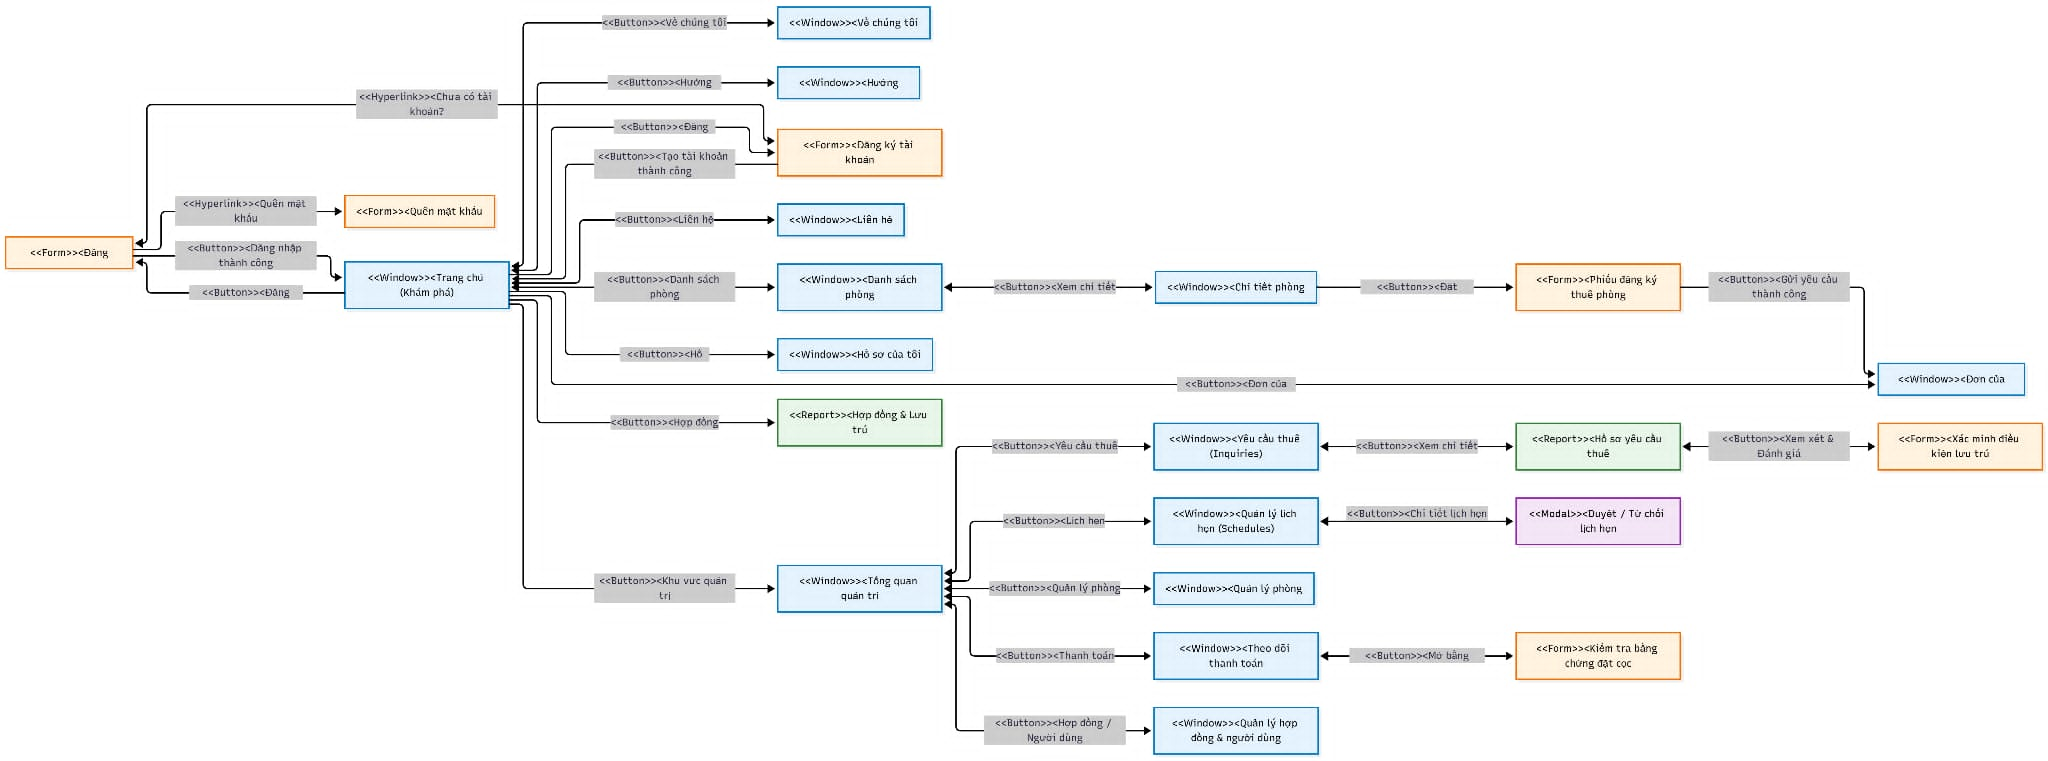
\includegraphics[width=0.98\textwidth]{images/WindowsNavigationDiagram}
    \caption{Sơ đồ điều hướng màn hình hệ thống HomeStay Dorm}
\end{figure}

\subsubsection*{Các nguyên lý thiết kế giao diện (UI Principles)}

Dựa trên cấu trúc frontend sử dụng \textbf{Angular 17/18+} và framework \textbf{Tailwind CSS}, hệ thống HomeStay Dorm tuân thủ nghiêm ngặt 4 nguyên lý thiết kế giao diện cốt lõi sau đây nhằm nâng cao trải nghiệm người dùng:

\subsubsection{Bố cục màn hình (Layout)}
Hệ thống sử dụng phương pháp phân chia khu vực (Screen Partitioning) kết hợp luồng thiết kế linh hoạt, giúp người dùng dễ dàng định vị thông tin và thao tác:
\begin{itemize}[leftmargin=*, nosep]
    \item \textbf{Vùng điều hướng (Navigation Area):} Được đặt ở thanh menu trên cùng (Navbar) đối với khu vực Public/Customer. Vùng này tự động thay đổi theo trạng thái đăng nhập, tích hợp Menu chọn ngôn ngữ (Anh/Việt) và Menu người dùng. Đối với khu vực Quản trị (Admin), hệ thống bổ sung \textbf{Sidebar bên trái} chứa các module chức năng chuyên sâu (\textit{Yêu cầu thuê, Lịch hẹn, Quản lý phòng, Thanh toán, Người dùng}).
    \item \textbf{Vùng thao tác (Workspace Area):} Không gian hiển thị trung tâm. Các biểu mẫu (\texttt{<<Form>>}) như \textit{Phiếu đăng ký thuê phòng} hay các vùng tra cứu dữ liệu (\texttt{<<Window>>}) được đặt ở trung tâm trong các thẻ (Cards) với nền bo góc, tạo đổ bóng tinh tế để tập trung tối đa sự chú ý.
    \item \textbf{Vùng thông tin \& Chân trang (Status/Footer Area):} Cung cấp các thông tin liên hệ tĩnh (Trụ sở: 227 Nguyễn Văn Cừ, Phường 4, Quận 5), các số hotline, email và giờ làm việc, hiển thị đồng nhất trên mọi màn hình.
\end{itemize}

\subsubsection{Nhận thức nội dung (Content Awareness)}
Hệ thống đảm bảo người dùng luôn biết rõ họ đang ở đâu, đang làm gì và trạng thái quy trình ra sao:
\begin{itemize}[leftmargin=*, nosep]
    \item \textbf{Tiêu đề và Phụ đề (Titles \& Subtitles):} Mỗi màn hình đều có ngữ cảnh rõ ràng. Ví dụ: Màn hình đặt phòng hiển thị \textit{``Phiếu đăng ký thuê phòng - Cho chúng tôi biết nhu cầu của bạn...''}; màn hình quản lý lịch hẹn có \textit{``Quản lý Lịch hẹn - Theo dõi và sắp xếp lịch xem phòng thực tế...''}.
    \item \textbf{Phản hồi trạng thái (State Feedback):} Tích hợp các huy hiệu (Badges) và mã màu (Color-coding) trạng thái thông minh theo thời gian thực. Ví dụ: Trạng thái \textit{Pending} dùng màu Vàng (Amber), \textit{Scheduled / Paid} dùng màu Xanh (Emerald), và \textit{Cancelled / Rejected} dùng màu Đỏ (Red). Hệ thống ánh xạ chính xác trạng thái từ Database sang UI thông qua file \texttt{vi.json}.
    \item \textbf{Chỉ báo tiến trình \& Empty State (Loading / Empty States):} Xây dựng Loading overlay toàn cục với logo và Slogan \textit{``Nurturing Your Journey, Building Your Home.''} kết hợp vòng xoay (spinner). Ngoài ra, khi không có dữ liệu, hệ thống luôn có Empty State rõ ràng (ví dụ: \textit{``Không tìm thấy lịch hẹn cho các bộ lọc đã chọn''}).
\end{itemize}

\subsubsection{Tính nhất quán (Consistency)}
\begin{itemize}[leftmargin=*, nosep]
    \item \textbf{Đồng bộ Thuật ngữ (Terminology):} Nhờ sử dụng kiến trúc đa ngôn ngữ \texttt{@ngx-translate} (file \texttt{vi.json} / \texttt{en.json}), các từ ngữ nghiệp vụ mang tính đồng nhất tuyệt đối trên mọi màn hình. Cụm từ \textit{``Chi nhánh''}, \textit{``Phòng đôi''}, \textit{``Phòng bốn''}, \textit{``Bằng chứng đặt cọc''} được dùng xuyên suốt.
    \item \textbf{Đồng bộ Tương tác (Interaction \& Visual Consistency):} Sử dụng mã màu thương hiệu \texttt{\#264893} cho các nút hành động chính (Primary Buttons). Hiệu ứng \textit{Hover} được dùng đồng nhất (class \texttt{.hover-effect}). Các thao tác quan trọng hoặc mang tính phá hủy (Từ chối, Hủy đơn, Duyệt lịch) đều sử dụng \textbf{Modal Overlay} với nền mờ tối màu để yêu cầu người dùng xác nhận lần cuối.
\end{itemize}

\subsubsection{Tối thiểu hóa nỗ lực (Minimal User Effort)}
Hệ thống được thiết kế để hạn chế tối đa số thao tác thừa, giúp người dùng làm việc nhanh chóng, hiệu quả:
\begin{itemize}[leftmargin=*, nosep]
    \item \textbf{Tự động điền dữ liệu (Prefilled Data):} Tại chức năng \textit{Đăng ký thuê phòng}, nếu khách hàng chọn Đặt phòng từ trang \textit{Chi tiết phòng}, hệ thống tự động ghi nhận \texttt{room\_id} và \texttt{branch\_name} qua Angular Router State, người dùng không cần phải chọn lại. Tương tự, tại trang \textit{Thanh toán} của Admin, Form "Tạo yêu cầu đặt cọc" tự động điền sẵn tên khách, chi nhánh, phòng và số tiền.
    \item \textbf{Luồng biểu mẫu đa bước (Wizard Form Optimization):} Biểu mẫu \textit{``Phiếu đăng ký thuê phòng''} thay vì hiển thị thành một trang dài, đã được chia nhỏ thành 4 bước (Steps) rõ ràng thông qua biến \texttt{currentPage} (Chọn phòng $\rightarrow$ Tải CCCD $\rightarrow$ Xác nhận lịch $\rightarrow$ Hoàn tất). Có thanh báo số bước giúp người dùng không bị ngợp thông tin.
    \item \textbf{Bộ lọc tự động và Tác vụ nhanh (Smart Filters \& Quick Actions):} Các màn hình tra cứu của Admin và Customer đều cung cấp thanh tìm kiếm (Search bar) debounce tự động và các Dropdown lọc theo Chi nhánh, Trạng thái (được xử lý tức thời không cần tải lại trang).
\end{itemize}



\newpage
\subsection{Kiến trúc 3 lớp}
\label{sec:three-layer-architecture}

Hệ thống quản lý kí túc xá được chia thành ba tầng với trách nhiệm rõ ràng: lớp
giao diện, lớp nghiệp vụ và lớp dữ liệu. Mô hình này giúp giảm sự phụ thuộc giữa
giao diện, xử lý logic và lưu trữ, từ đó làm cho hệ thống dễ kiểm thử, dễ bảo trì
và dễ mở rộng hơn. Trong dự án ký túc xá, kiến trúc 3 lớp cũng khớp với cách
phân tích BCE ở mức khái niệm và cách triển khai Express.js ở backend.

\subsubsection{Lớp giao diện}
Đây là nơi người dùng tương tác trực tiếp với hệ thống. Các màn hình
Angular chịu trách nhiệm hiển thị dữ liệu, thu nhận thao tác người dùng và gửi
yêu cầu đến backend thông qua API. Lớp này không xử lý quy tắc nghiệp vụ, mà chỉ
tập trung vào giao diện, trải nghiệm người dùng và việc phản hồi thông tin một
cách rõ ràng, nhất quán.

\begin{itemize}
    \item Ví dụ: \texttt{BookingView}, \texttt{PaymentView}, \texttt{ContractView}, \texttt{CheckoutView}, \texttt{RoomView}.
    \item Nhiệm vụ chính: hiển thị danh sách phòng, form đặt cọc, màn hình thanh toán, thông tin hợp đồng và biểu mẫu trả phòng.
    \item Nguyên tắc: không chứa logic nghiệp vụ và không truy cập dữ liệu trực tiếp.
\end{itemize}

\subsubsection{Lớp nghiệp vụ}
Lớp nghiệp vụ xử lý các quy tắc cốt lõi của hệ thống. Đây là nơi kiểm tra trạng
thái phòng, xác nhận thông tin khách hàng, tính tiền đặt cọc, quản lý hợp đồng,
điều phối quy trình trả phòng và tính toán hoàn tiền. Trong backend, lớp này được
triển khai chủ yếu qua các controller và service để đảm bảo luồng xử lý được tách
biệt khỏi giao diện và dữ liệu.

\begin{itemize}
    \item Ví dụ: \texttt{BookingController}, \texttt{PaymentController}, \texttt{ContractController}, \texttt{CheckoutController}, \texttt{RefundCalculator}, \texttt{SchedulerController}.
    \item Nhiệm vụ chính: kiểm tra tính hợp lệ của yêu cầu, cập nhật trạng thái phòng/giường, xử lý đặt cọc, lập hợp đồng và đối soát chi phí.
    \item Nguyên tắc: nhận yêu cầu từ lớp trình bày, làm việc với lớp dữ liệu qua service/repository và không trực tiếp đảm nhiệm giao diện.
\end{itemize}

\subsubsection{Lớp dữ liệu}
Lớp dữ liệu lưu trữ các thực thể và trạng thái bền vững của hệ thống. Các đối
tượng trong lớp này phản ánh trực tiếp dữ liệu nghiệp vụ như khách hàng, nhân
viên, phòng, giường, đặt cọc, thanh toán, hợp đồng và biên bản thanh lý. Ở mức
triển khai, lớp này kết nối với cơ sở dữ liệu Supabase/PostgreSQL thông qua mô
hình dữ liệu và các bảng tương ứng.

\begin{itemize}
    \item Ví dụ: \texttt{Customer}, \texttt{Employee}, \texttt{Room}, \texttt{Bed}, \texttt{DepositRequest}, \texttt{Payment}, \texttt{Contract}, \texttt{CheckoutRequest}, \texttt{Settlement}.
    \item Nhiệm vụ chính: biểu diễn dữ liệu nghiệp vụ, lưu trạng thái và cung cấp cấu trúc cho việc đọc/ghi dữ liệu.
    \item Nguyên tắc: không điều phối luồng xử lý và không chứa logic ra quyết định phức tạp.
\end{itemize}


\begin{figure}[H]
    \centering
    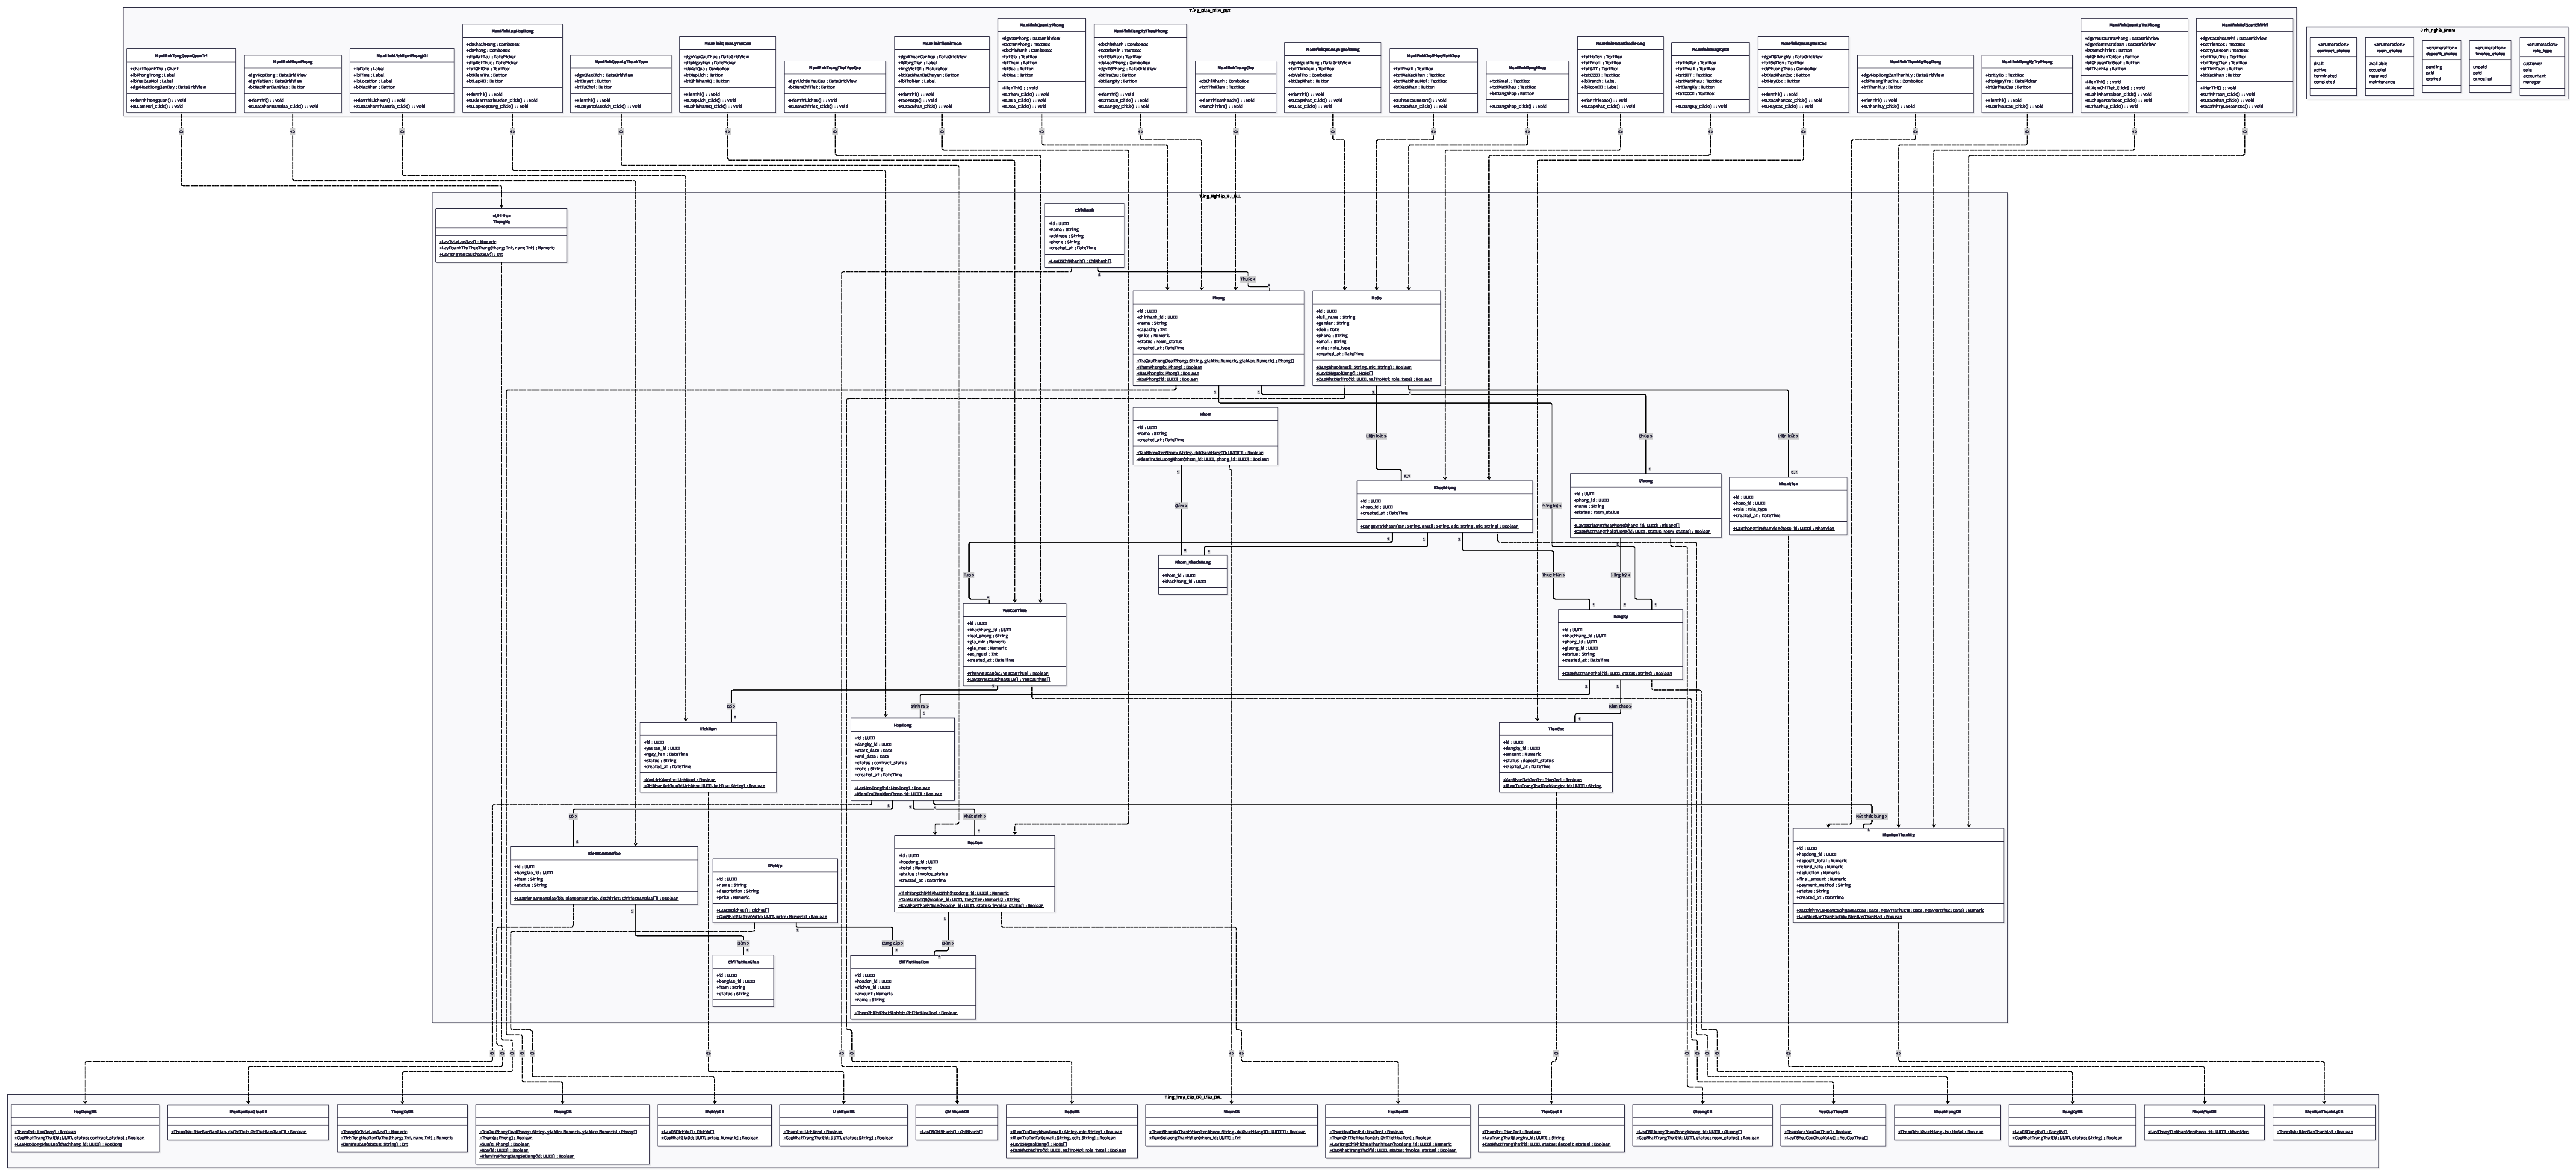
\includegraphics[width=0.98\textwidth]{images/3-Layer.pdf}
    \caption{Sơ đồ điều hướng màn hình hệ thống HomeStay Dorm}
\end{figure}





\newpage
\subsection{Sequence Diagram}
\label{sec:sequence-diagrams}
% ----------------------------------------------------------------
% SUC1
% ----------------------------------------------------------------
\subsubsection{SUC1 -- Đăng nhập}
\begin{figure}[H]
    \centering
    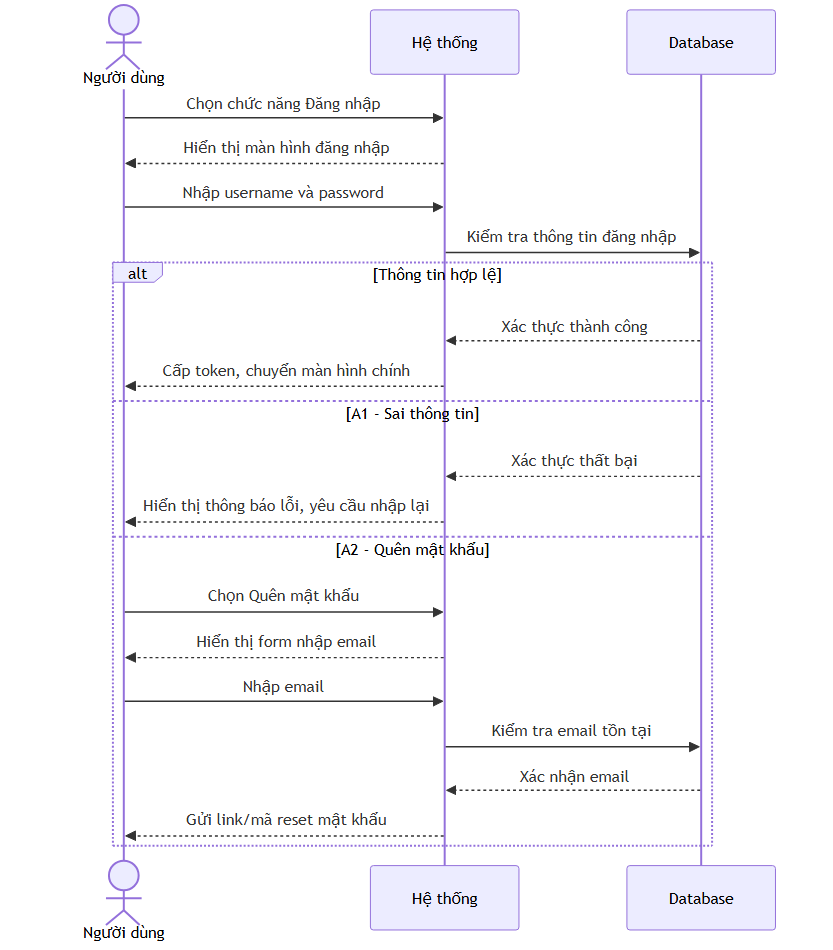
\includegraphics[width=\textwidth]{images/sequence_diagrams/SUC1_DangNhap.png}
    \caption{Sơ đồ tuần tự -- SUC1: Đăng nhập}
    \label{fig:seq-suc1}
\end{figure}

% ----------------------------------------------------------------
% SUC2
% ----------------------------------------------------------------
\subsubsection{SUC2 -- Đăng ký thuê phòng}
\begin{figure}[H]
    \centering
    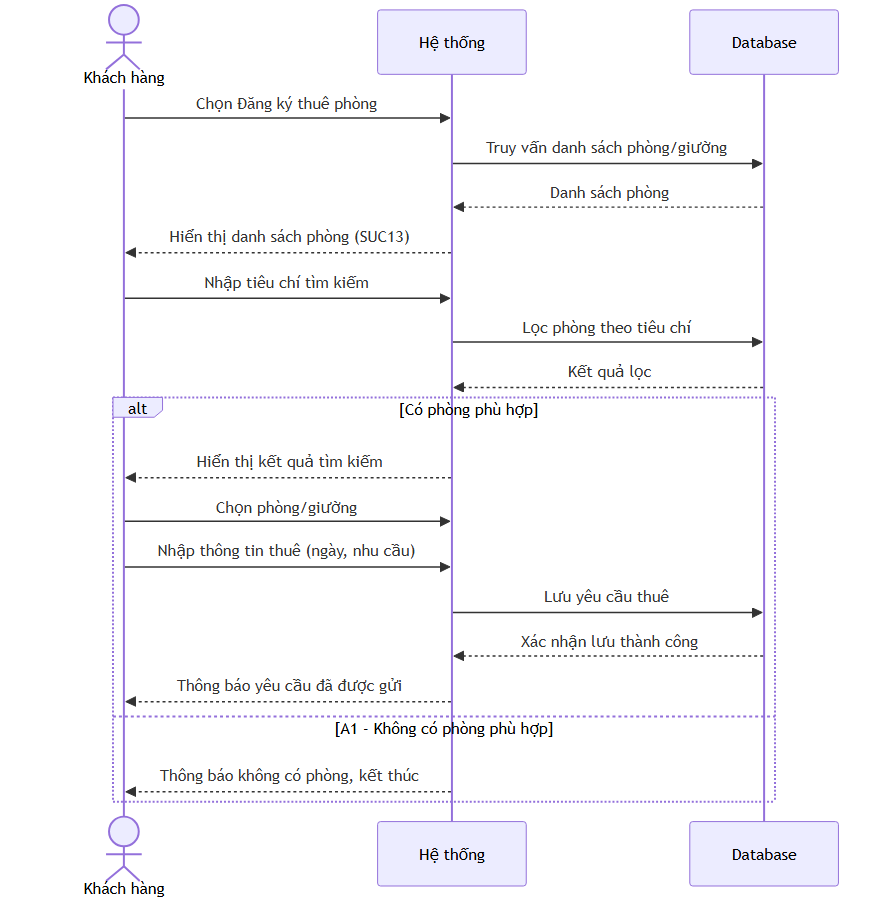
\includegraphics[width=\textwidth]{images/sequence_diagrams/SUC2_DangKyThuePhong.png}
    \caption{Sơ đồ tuần tự -- SUC2: Đăng ký thuê phòng}
    \label{fig:seq-suc2}
\end{figure}

% ----------------------------------------------------------------
% SUC3
% ----------------------------------------------------------------
\subsubsection{SUC3 -- Quản lý đăng ký thuê phòng}
\begin{figure}[H]
    \centering
    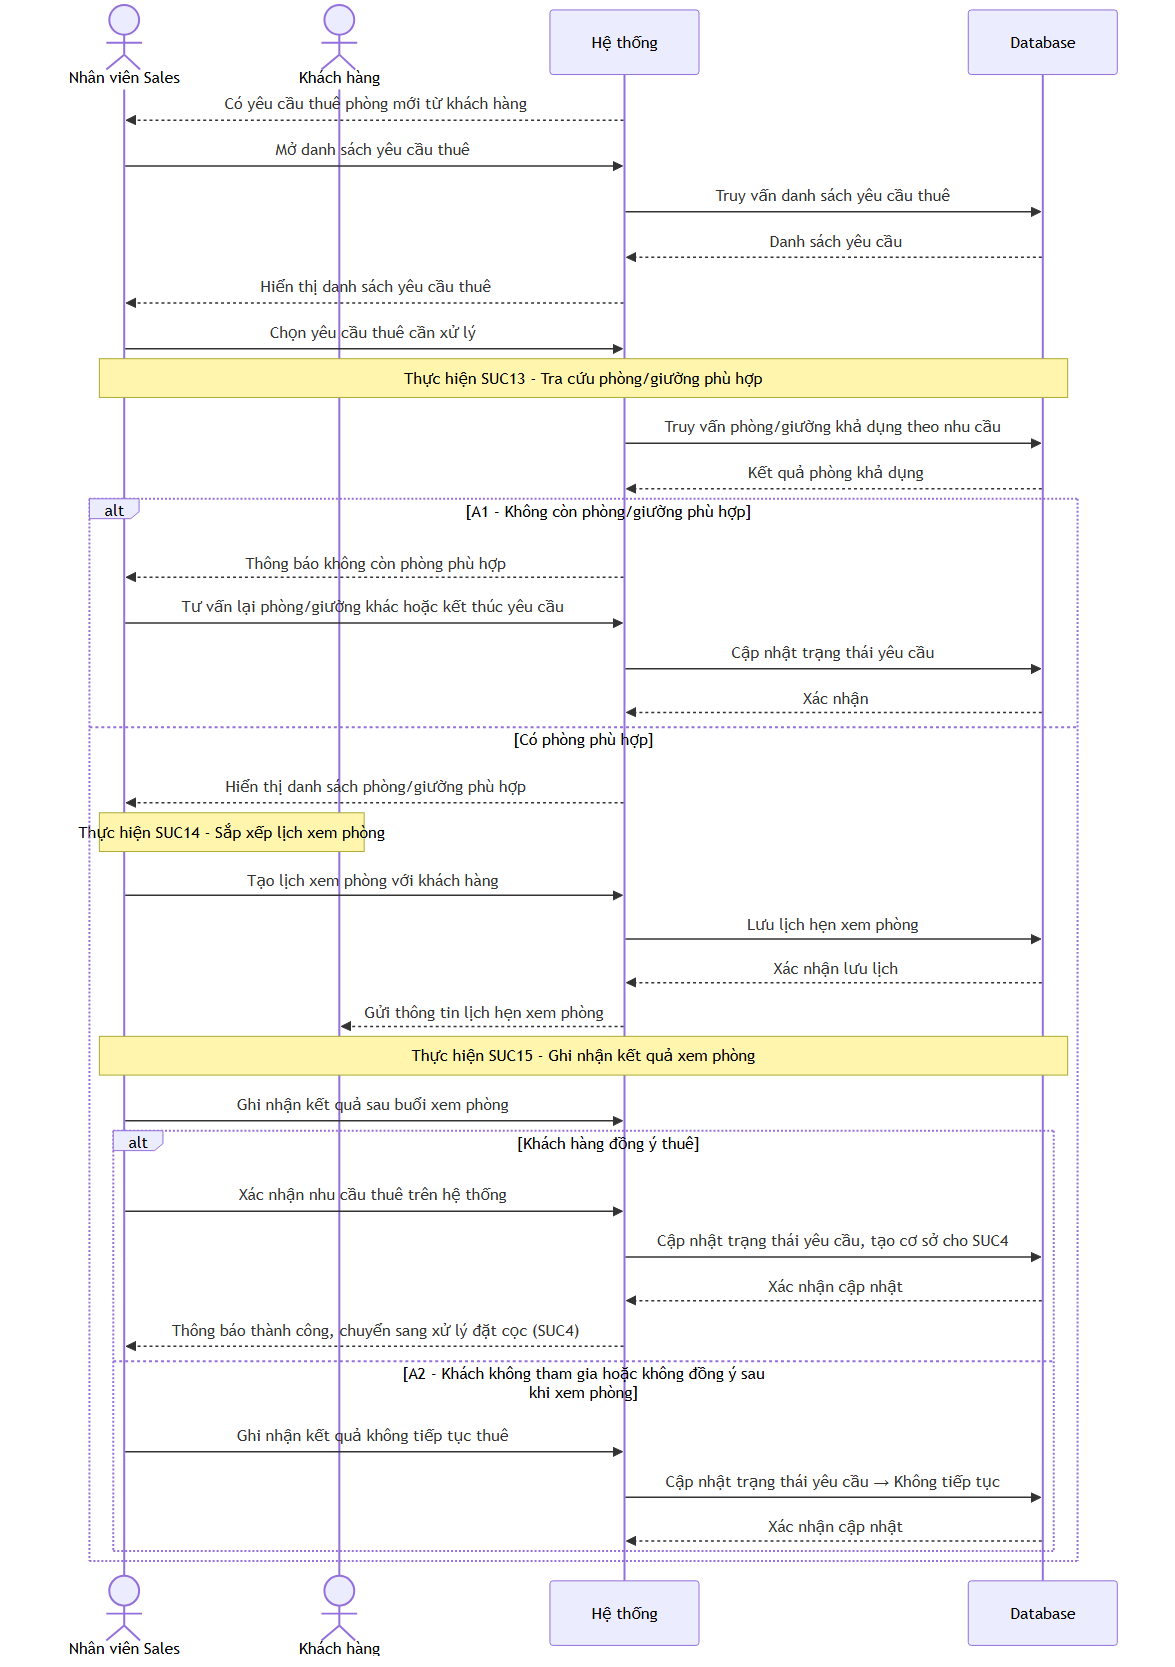
\includegraphics[width=\textwidth]{images/sequence_diagrams/SUC3_QuanLyDangKyThue.png}
    \caption{Sơ đồ tuần tự -- SUC3: Quản lý đăng ký thuê phòng}
    \label{fig:seq-suc3}
\end{figure}

% ----------------------------------------------------------------
% SUC4
% ----------------------------------------------------------------
\subsubsection{SUC4 -- Quản lý đặt cọc}
\begin{figure}[H]
    \centering
    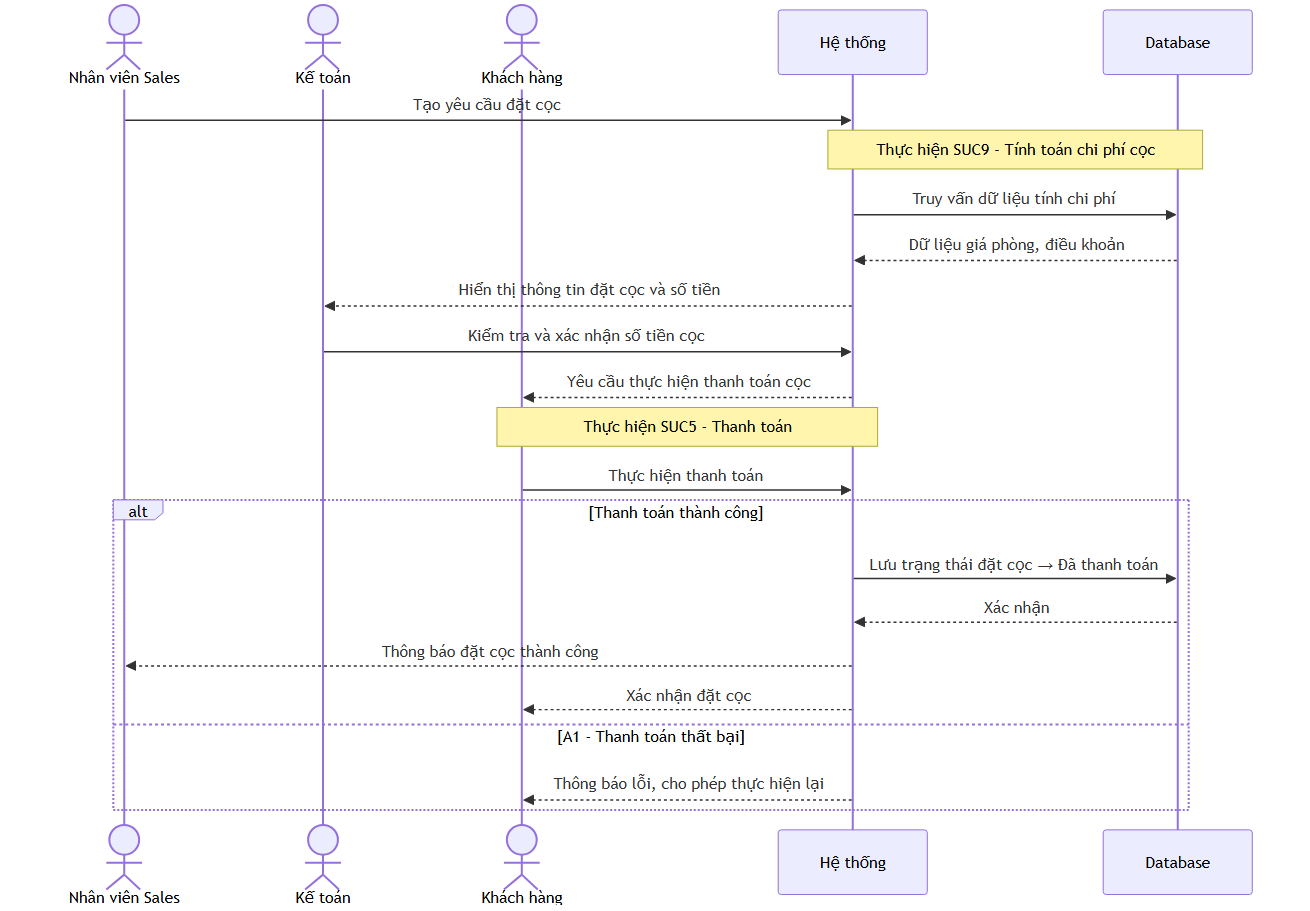
\includegraphics[width=\textwidth]{images/sequence_diagrams/SUC4_QuanLyDatCoc.png}
    \caption{Sơ đồ tuần tự -- SUC4: Quản lý đặt cọc}
    \label{fig:seq-suc4}
\end{figure}

% ----------------------------------------------------------------
% SUC5
% ----------------------------------------------------------------
\subsubsection{SUC5 -- Thanh toán}
\begin{figure}[H]
    \centering
    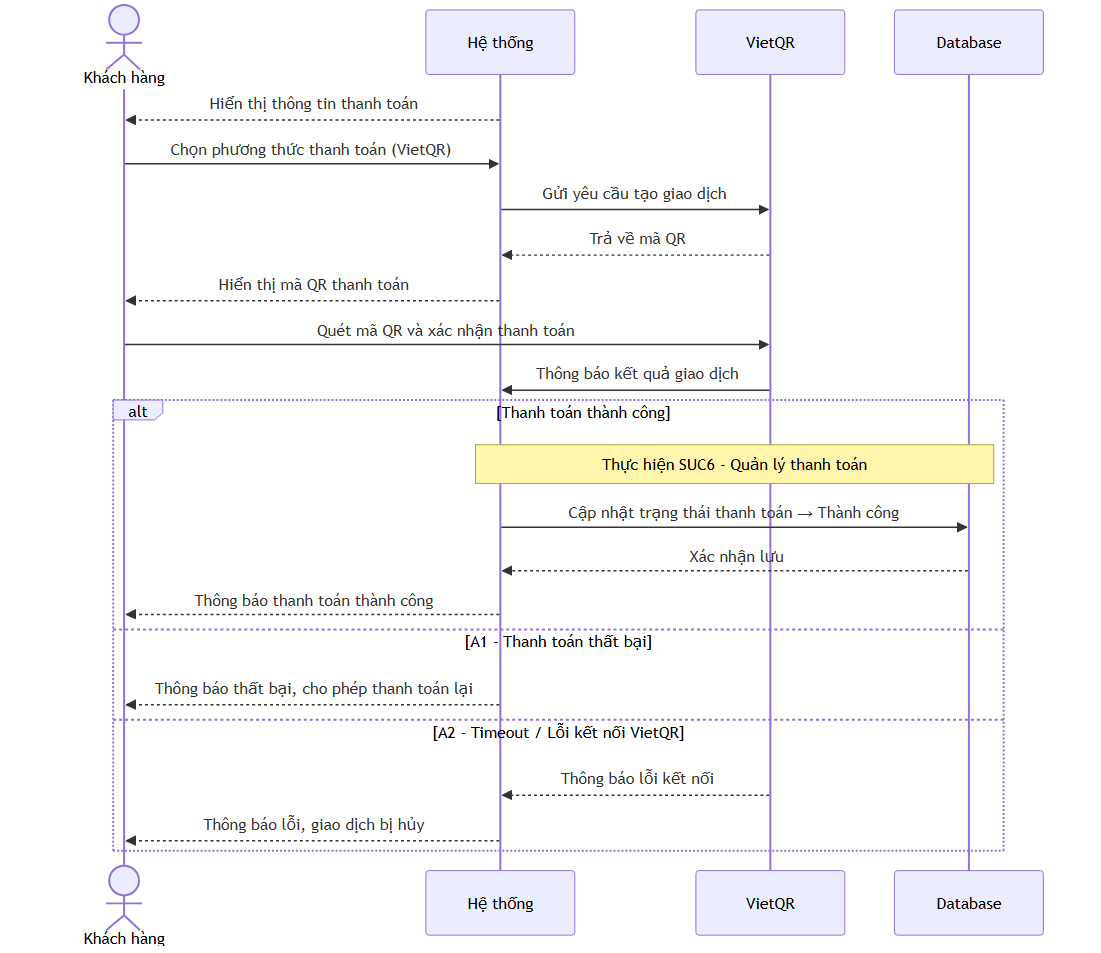
\includegraphics[width=\textwidth]{images/sequence_diagrams/SUC5_ThanhToan.png}
    \caption{Sơ đồ tuần tự -- SUC5: Thanh toán}
    \label{fig:seq-suc5}
\end{figure}

% ----------------------------------------------------------------
% SUC6
% ----------------------------------------------------------------
\subsubsection{SUC6 -- Quản lý thanh toán}
\begin{figure}[H]
    \centering
    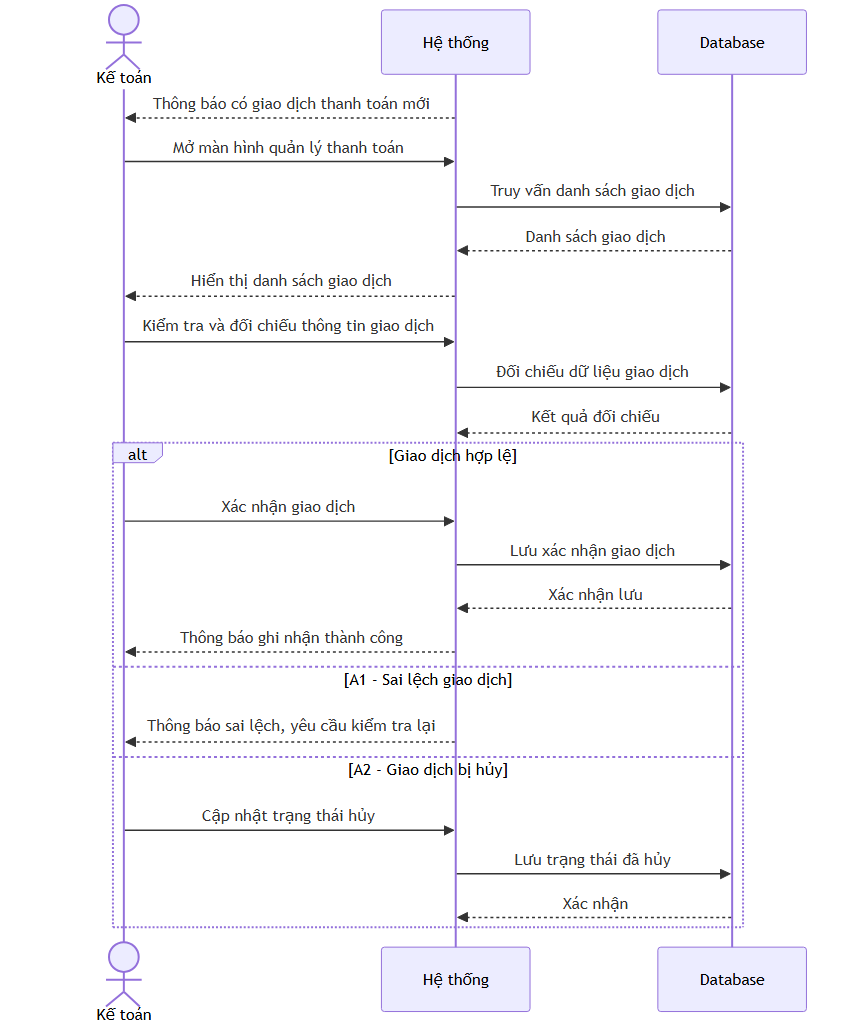
\includegraphics[width=\textwidth]{images/sequence_diagrams/SUC6_QuanLyThanhToan.png}
    \caption{Sơ đồ tuần tự -- SUC6: Quản lý thanh toán}
    \label{fig:seq-suc6}
\end{figure}

% ----------------------------------------------------------------
% SUC7
% ----------------------------------------------------------------
\subsubsection{SUC7 -- Quản lý hợp đồng}
\begin{figure}[H]
    \centering
    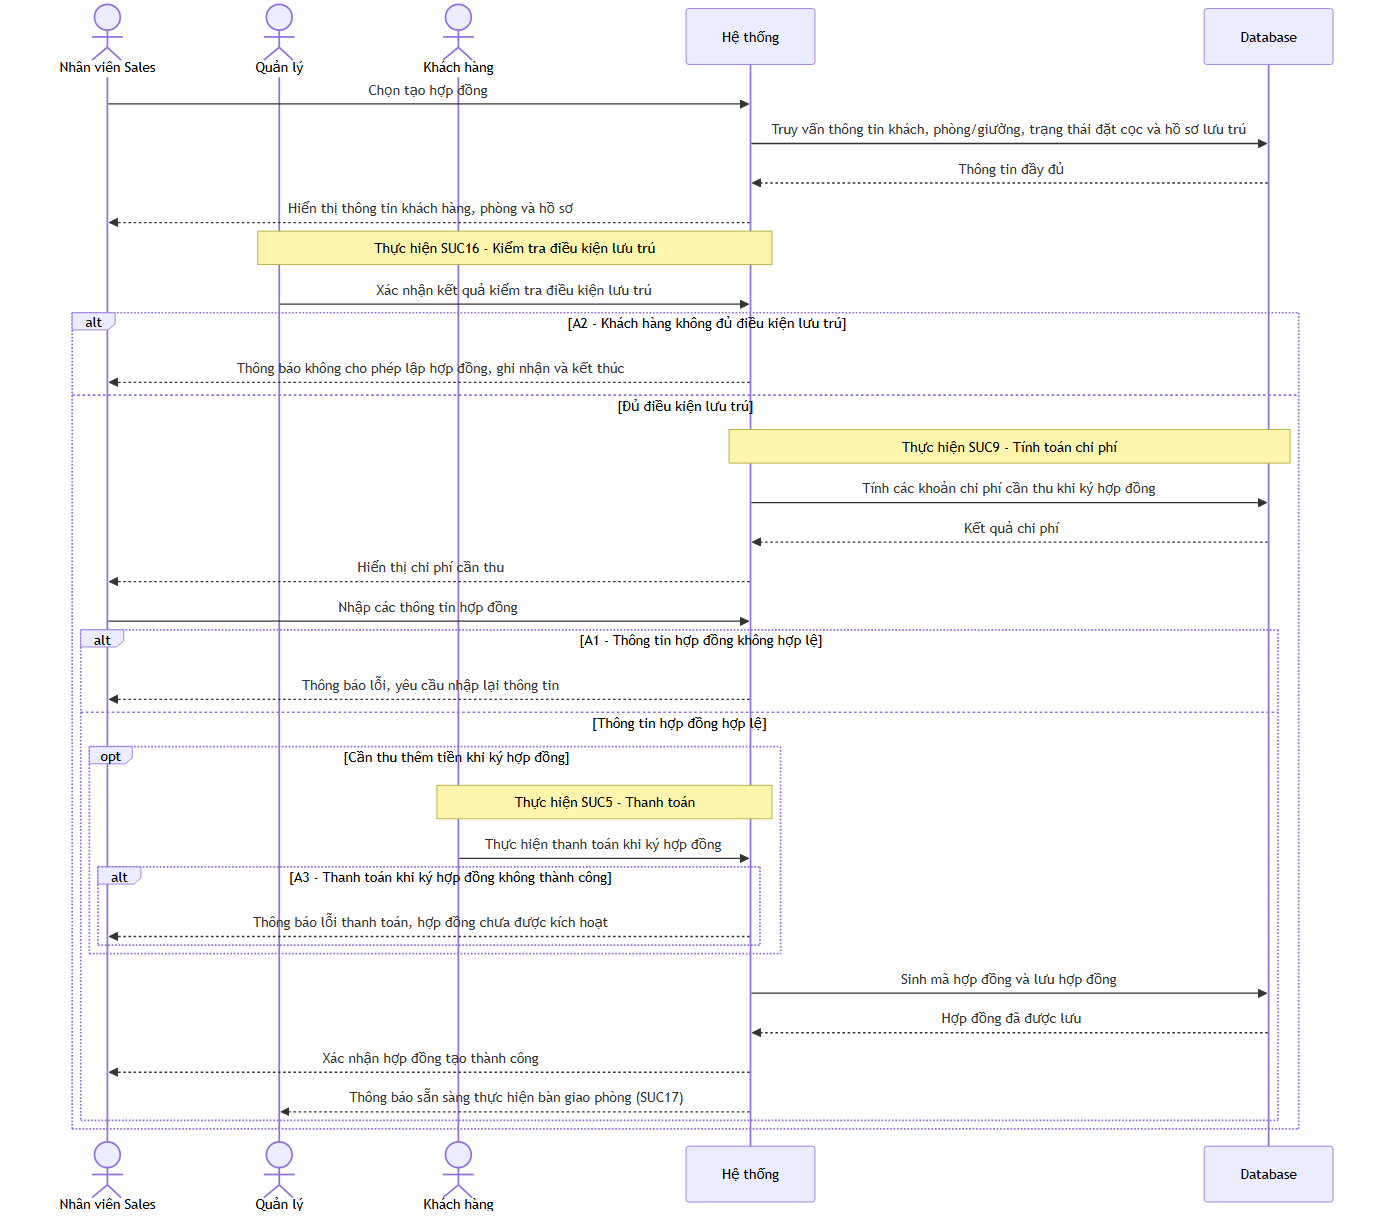
\includegraphics[width=\textwidth]{images/sequence_diagrams/SUC7_QuanLyHopDong.png}
    \caption{Sơ đồ tuần tự -- SUC7: Quản lý hợp đồng}
    \label{fig:seq-suc7}
\end{figure}

% ----------------------------------------------------------------
% SUC8
% ----------------------------------------------------------------
\subsubsection{SUC8 -- Đối soát chi phí}
\begin{figure}[H]
    \centering
    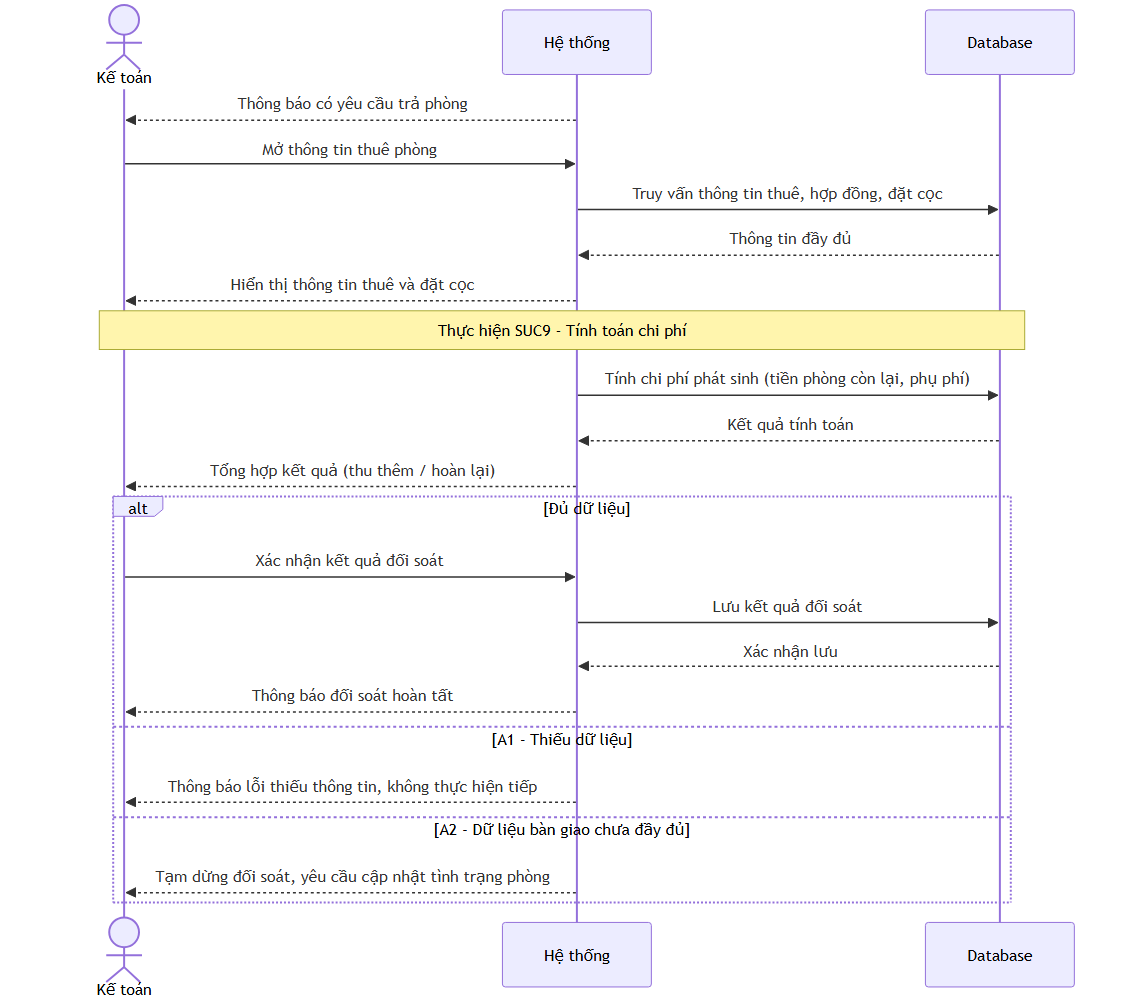
\includegraphics[width=\textwidth]{images/sequence_diagrams/SUC8_DoiSoatChiPhi.png}
    \caption{Sơ đồ tuần tự -- SUC8: Đối soát chi phí}
    \label{fig:seq-suc8}
\end{figure}

% ----------------------------------------------------------------
% SUC9
% ----------------------------------------------------------------
\subsubsection{SUC9 -- Tính toán chi phí}
\begin{figure}[H]
    \centering
    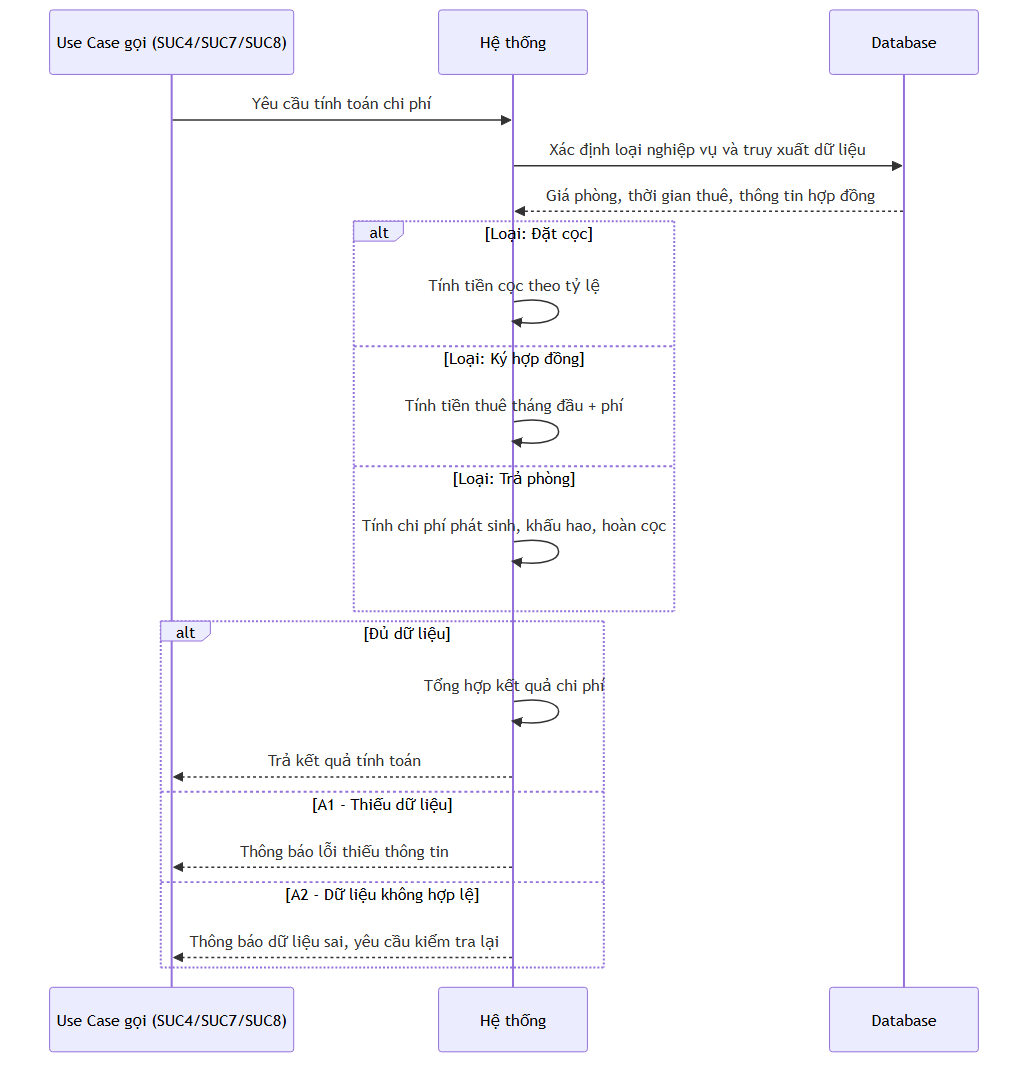
\includegraphics[width=\textwidth]{images/sequence_diagrams/SUC9_TinhToanChiPhi.png}
    \caption{Sơ đồ tuần tự -- SUC9: Tính toán chi phí}
    \label{fig:seq-suc9}
\end{figure}

% ----------------------------------------------------------------
% SUC10
% ----------------------------------------------------------------
\subsubsection{SUC10 -- Đăng ký trả phòng}
\begin{figure}[H]
    \centering
    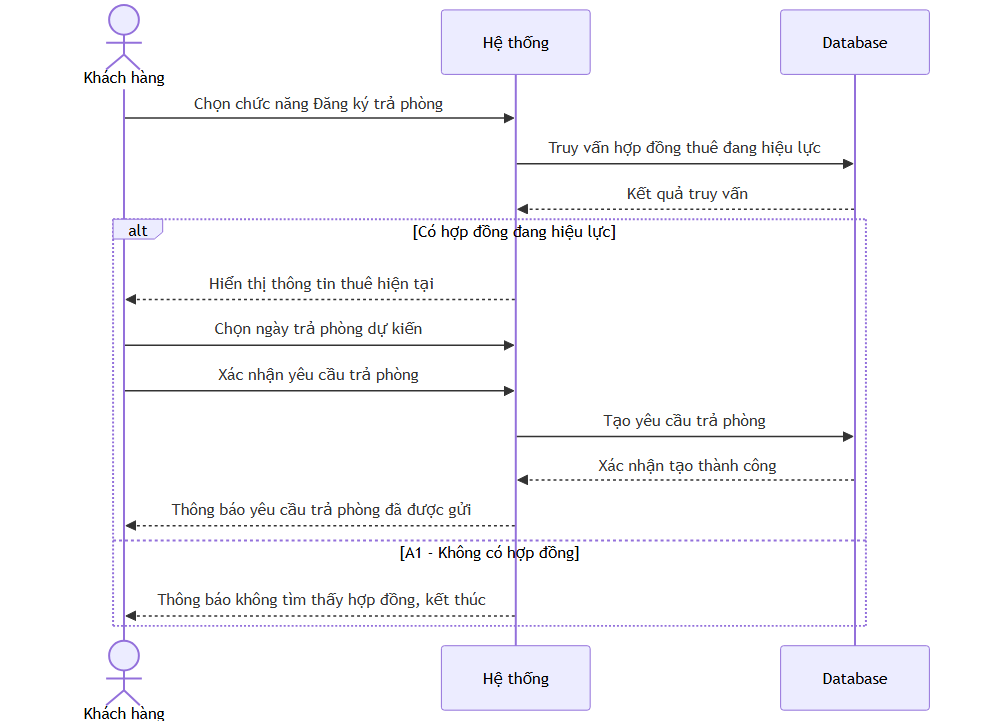
\includegraphics[width=\textwidth]{images/sequence_diagrams/SUC10_DangKyTraPhong.png}
    \caption{Sơ đồ tuần tự -- SUC10: Đăng ký trả phòng}
    \label{fig:seq-suc10}
\end{figure}

% ----------------------------------------------------------------
% SUC11
% ----------------------------------------------------------------
\subsubsection{SUC11 -- Quản lý đăng ký trả phòng}
\begin{figure}[H]
    \centering
    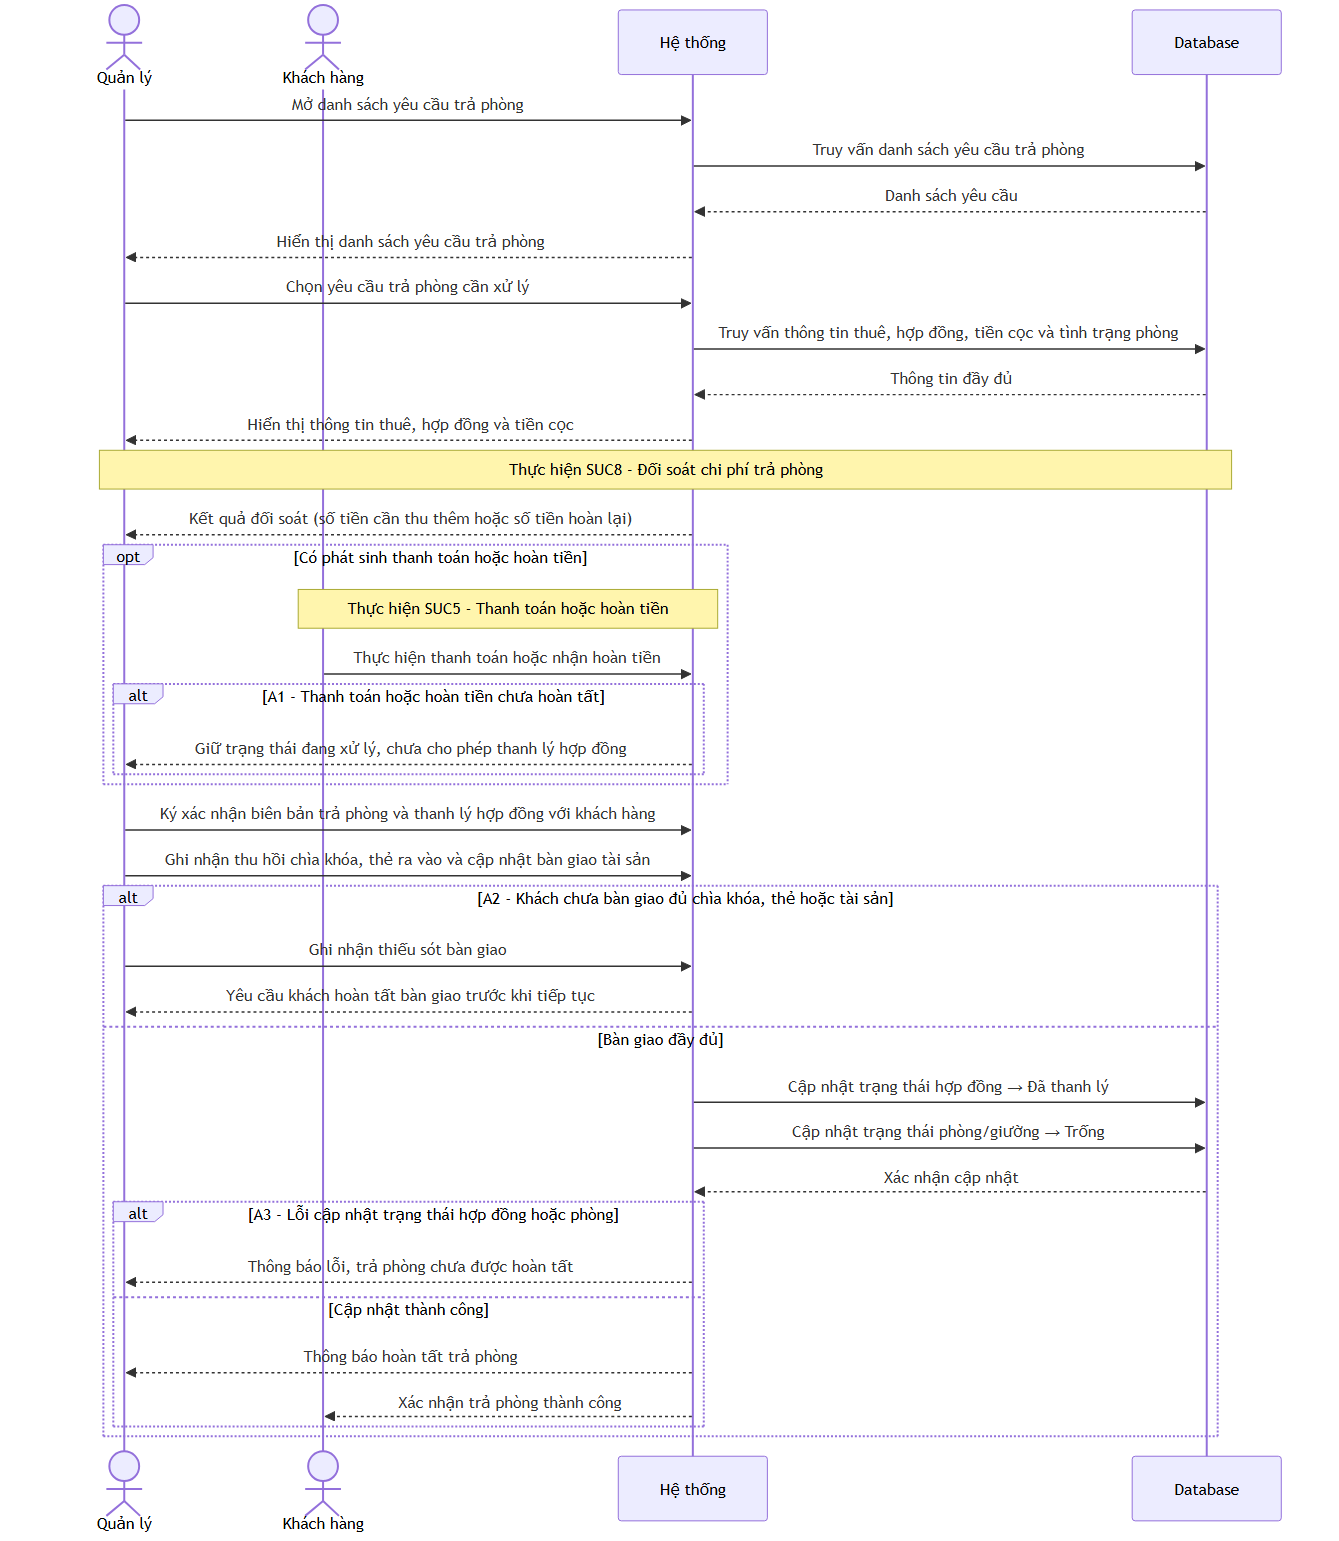
\includegraphics[width=\textwidth]{images/sequence_diagrams/SUC11_QuanLyTraPhong.png}
    \caption{Sơ đồ tuần tự -- SUC11: Quản lý đăng ký trả phòng}
    \label{fig:seq-suc11}
\end{figure}

% ----------------------------------------------------------------
% SUC12
% ----------------------------------------------------------------
\subsubsection{SUC12 -- Quản lý giường phòng}
\begin{figure}[H]
    \centering
    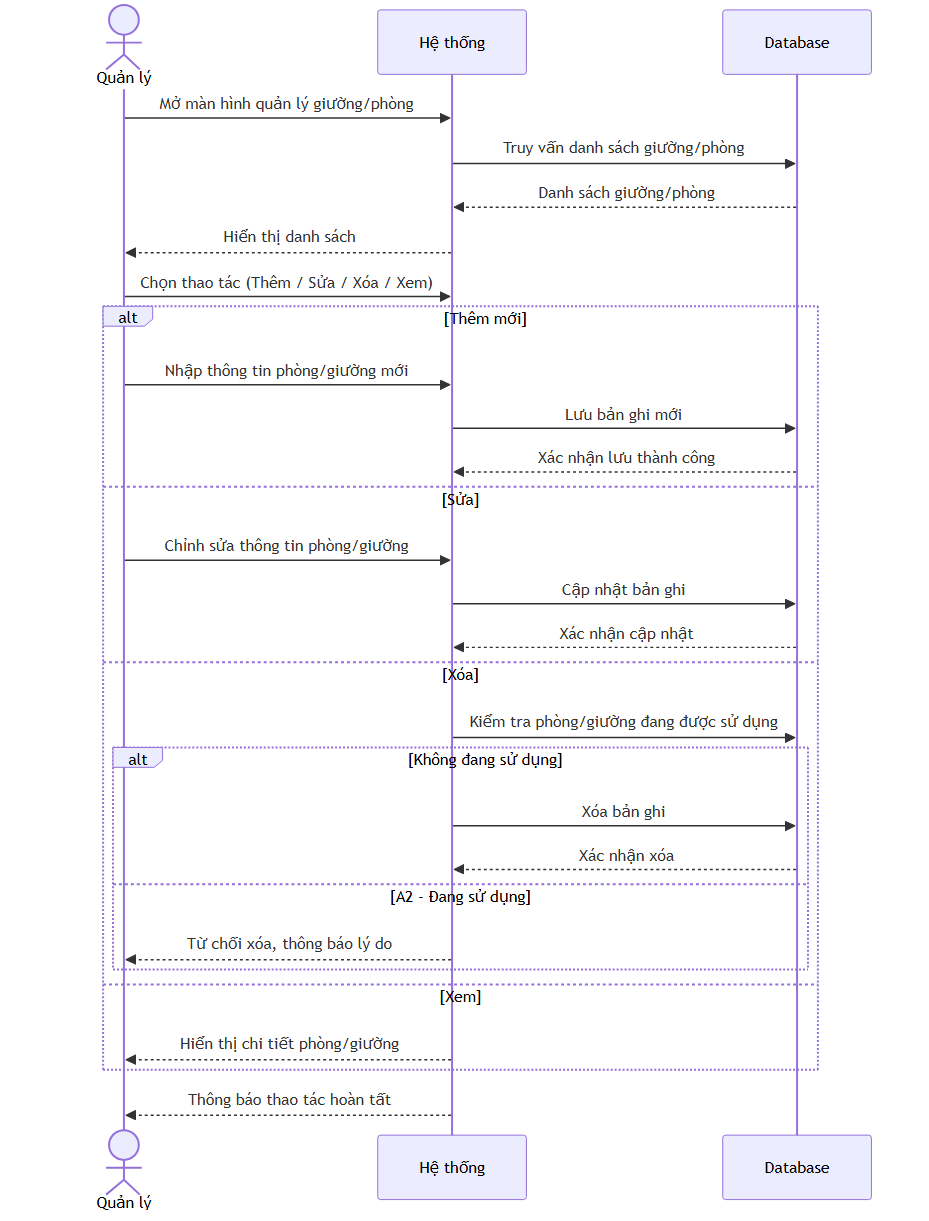
\includegraphics[width=\textwidth]{images/sequence_diagrams/SUC12_QuanLyGiuongPhong.png}
    \caption{Sơ đồ tuần tự -- SUC12: Quản lý giường phòng}
    \label{fig:seq-suc12}
\end{figure}

% ----------------------------------------------------------------
% SUC13
% ----------------------------------------------------------------
\subsubsection{SUC13 -- Xem/tra cứu giường phòng}
\begin{figure}[H]
    \centering
    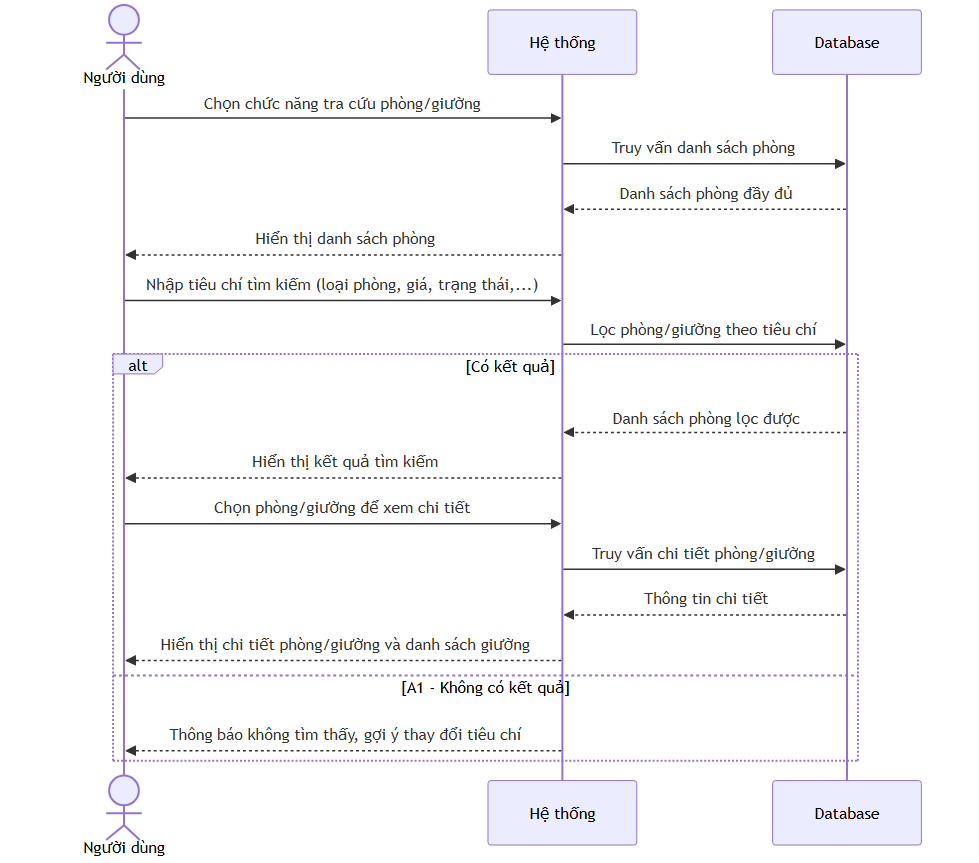
\includegraphics[width=\textwidth]{images/sequence_diagrams/SUC13_TraCuuPhong.png}
    \caption{Sơ đồ tuần tự -- SUC13: Xem/tra cứu giường phòng}
    \label{fig:seq-suc13}
\end{figure}

% ----------------------------------------------------------------
% SUC14
% ----------------------------------------------------------------
\subsubsection{SUC14 -- Sắp xếp lịch xem phòng}
\begin{figure}[H]
    \centering
    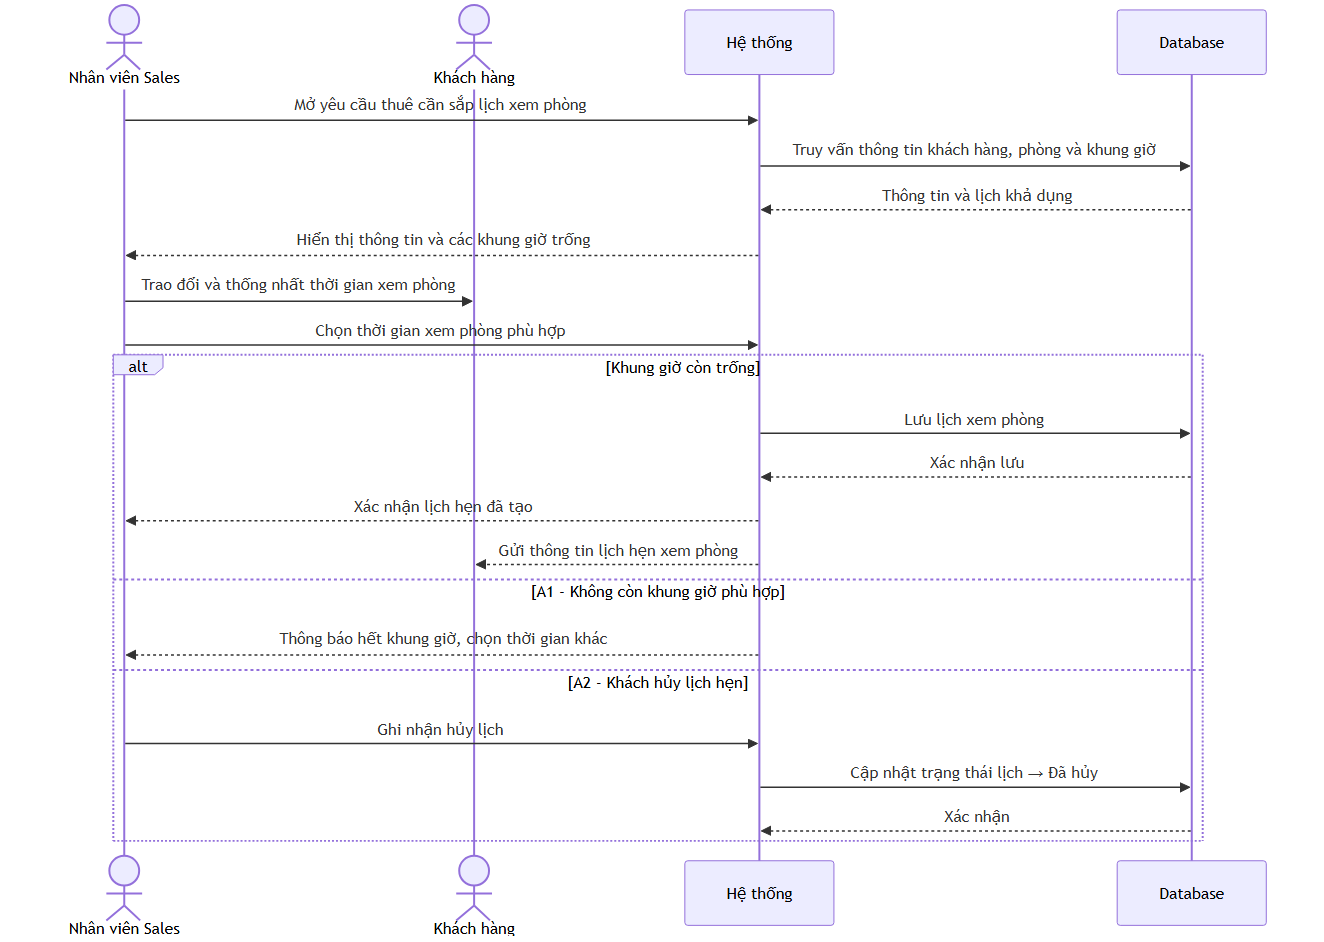
\includegraphics[width=\textwidth]{images/sequence_diagrams/SUC14_SapXepLichXemPhong.png}
    \caption{Sơ đồ tuần tự -- SUC14: Sắp xếp lịch xem phòng}
    \label{fig:seq-suc14}
\end{figure}

% ----------------------------------------------------------------
% SUC15
% ----------------------------------------------------------------
\subsubsection{SUC15 -- Ghi nhận kết quả xem phòng}
\begin{figure}[H]
    \centering
    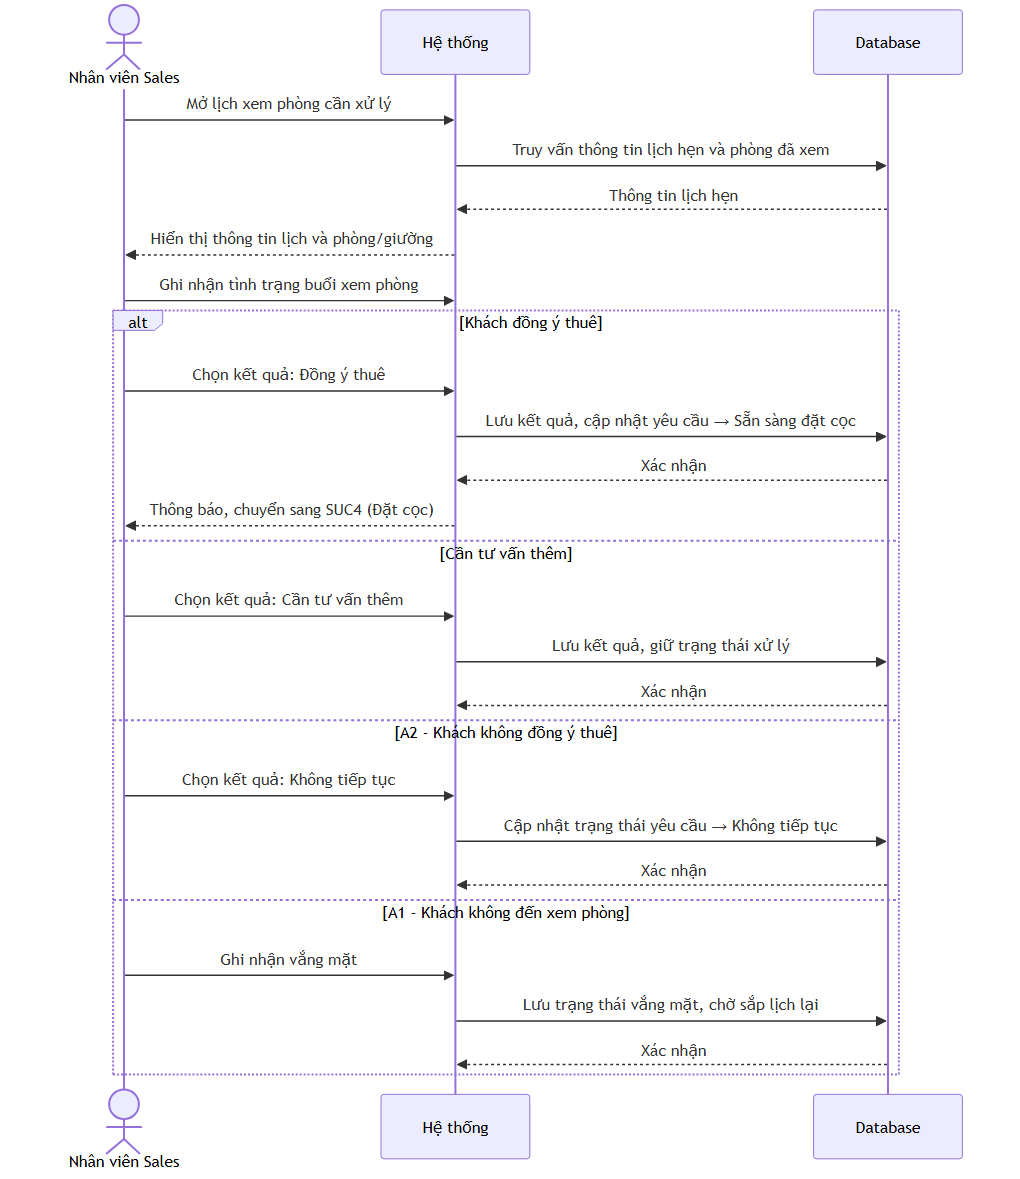
\includegraphics[width=\textwidth]{images/sequence_diagrams/SUC15_GhiNhanKetQuaXemPhong.png}
    \caption{Sơ đồ tuần tự -- SUC15: Ghi nhận kết quả xem phòng}
    \label{fig:seq-suc15}
\end{figure}

% ----------------------------------------------------------------
% SUC16
% ----------------------------------------------------------------
\subsubsection{SUC16 -- Kiểm tra điều kiện lưu trú}
\begin{figure}[H]
    \centering
    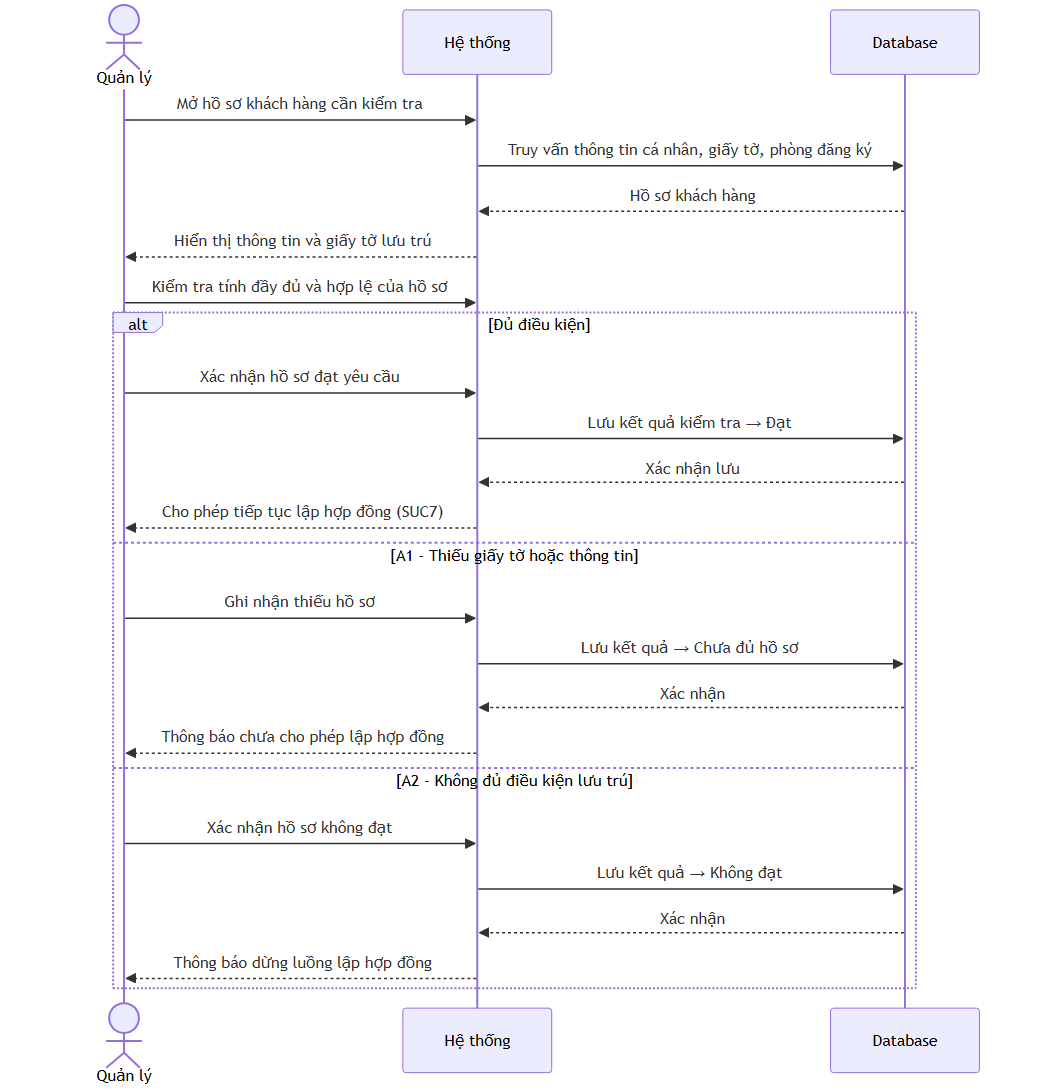
\includegraphics[width=\textwidth]{images/sequence_diagrams/SUC16_KiemTraDieuKienLuTru.png}
    \caption{Sơ đồ tuần tự -- SUC16: Kiểm tra điều kiện lưu trú}
    \label{fig:seq-suc16}
\end{figure}

% ----------------------------------------------------------------
% SUC17
% ----------------------------------------------------------------
\subsubsection{SUC17 -- Nhận phòng và bàn giao}
\begin{figure}[H]
    \centering
    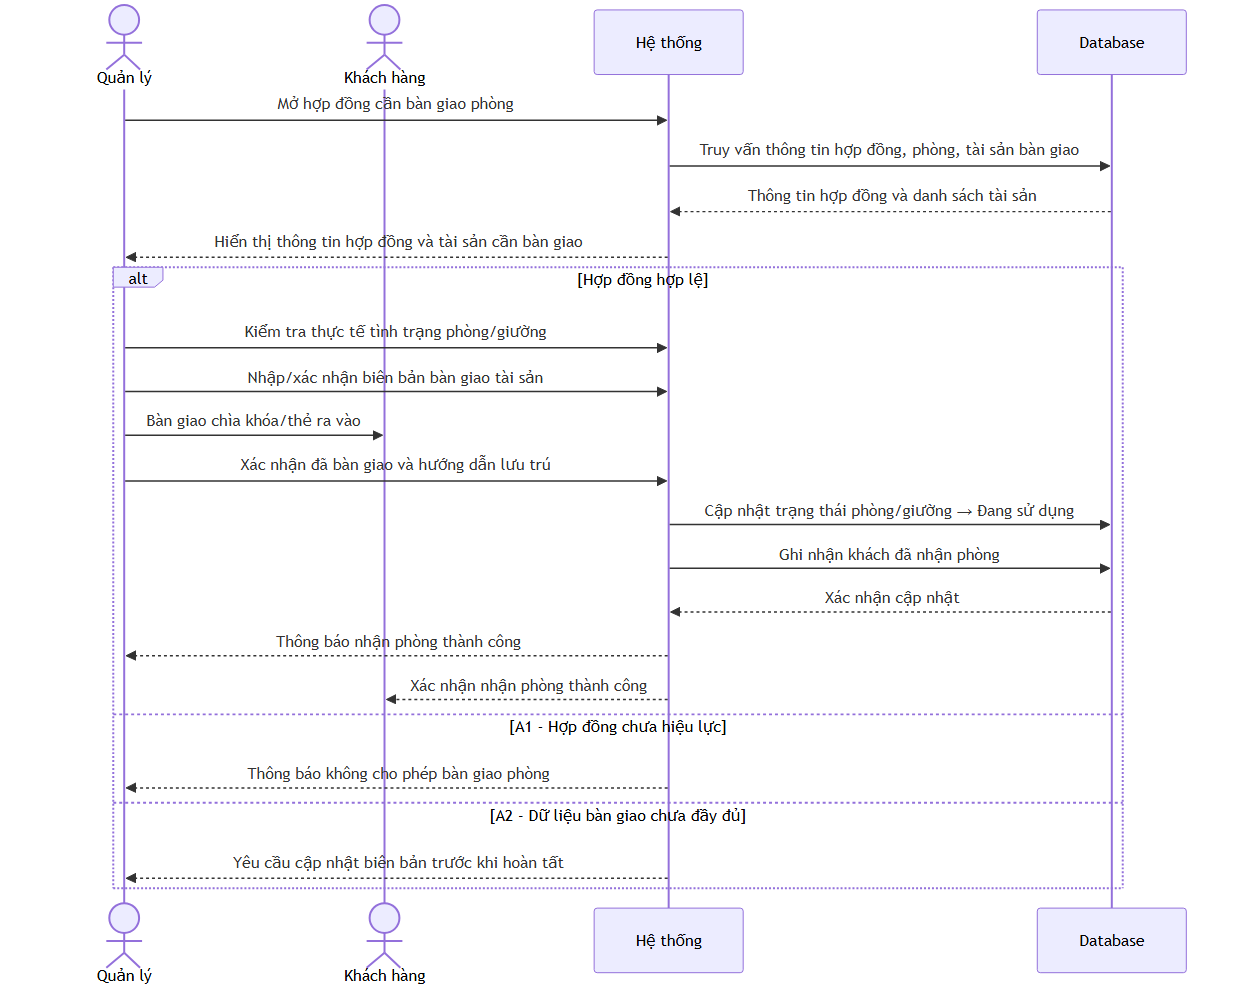
\includegraphics[width=\textwidth]{images/sequence_diagrams/SUC17_NhanPhongBanGiao.png}
    \caption{Sơ đồ tuần tự -- SUC17: Nhận phòng và bàn giao}
    \label{fig:seq-suc17}
\end{figure}

% ----------------------------------------------------------------
% SUC18
% ----------------------------------------------------------------
\subsubsection{SUC18 -- Đăng ký tài khoản khách hàng}
\begin{figure}[H]
    \centering
    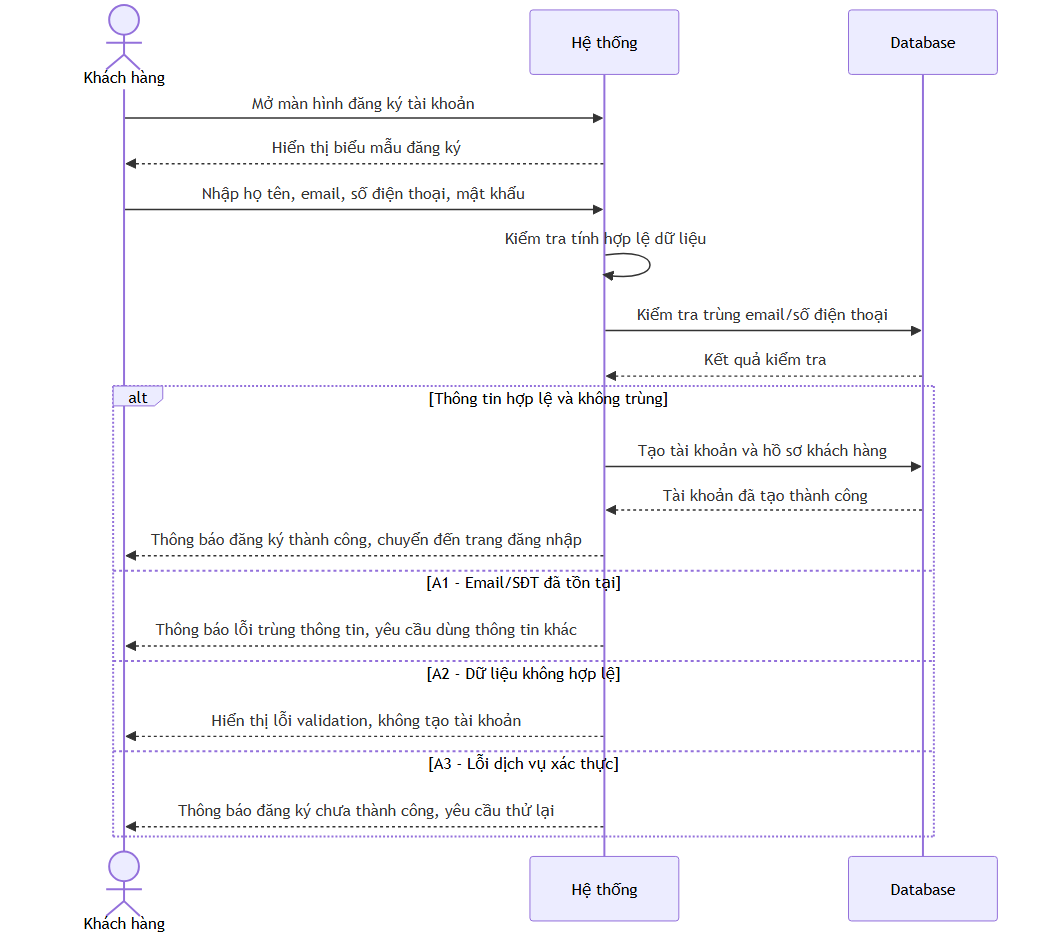
\includegraphics[width=\textwidth]{images/sequence_diagrams/SUC18_DangKyTaiKhoan.png}
    \caption{Sơ đồ tuần tự -- SUC18: Đăng ký tài khoản khách hàng}
    \label{fig:seq-suc18}
\end{figure}

% ----------------------------------------------------------------
% SUC19
% ----------------------------------------------------------------
\subsubsection{SUC19 -- Quản lý người dùng}
\begin{figure}[H]
    \centering
    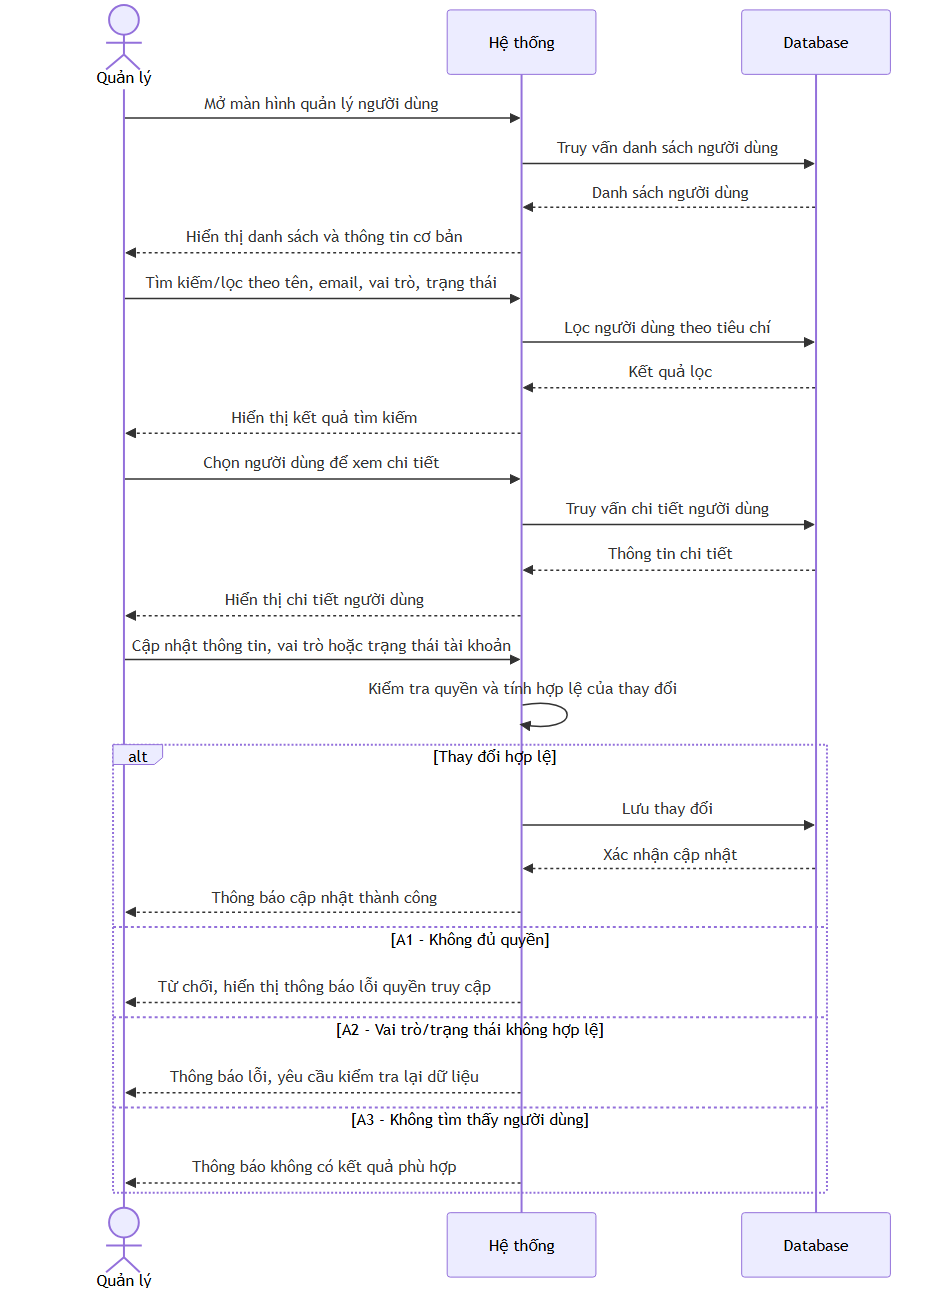
\includegraphics[width=\textwidth]{images/sequence_diagrams/SUC19_QuanLyNguoiDung.png}
    \caption{Sơ đồ tuần tự -- SUC19: Quản lý người dùng}
    \label{fig:seq-suc19}
\end{figure}

% ----------------------------------------------------------------
% SUC20
% ----------------------------------------------------------------
\subsubsection{SUC20 -- Xem trạng thái yêu cầu thuê/đặt phòng}
\begin{figure}[H]
    \centering
    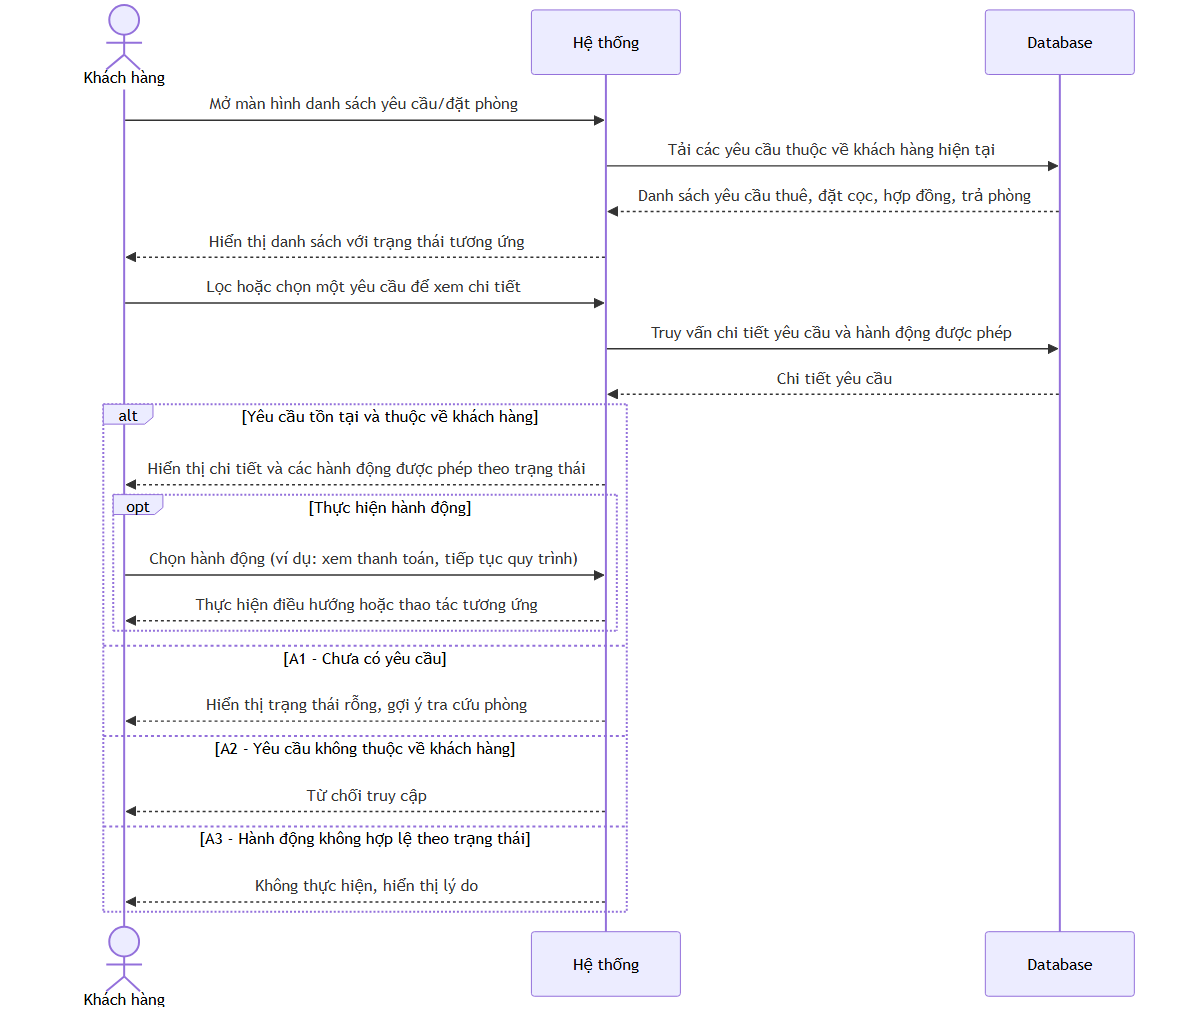
\includegraphics[width=\textwidth]{images/sequence_diagrams/SUC20_XemTrangThaiYeuCau.png}
    \caption{Sơ đồ tuần tự -- SUC20: Xem trạng thái yêu cầu thuê/đặt phòng}
    \label{fig:seq-suc20}
\end{figure}

% ----------------------------------------------------------------
% SUC21
% ----------------------------------------------------------------
\subsubsection{SUC21 -- Tổng quan quản trị}
\begin{figure}[H]
    \centering
    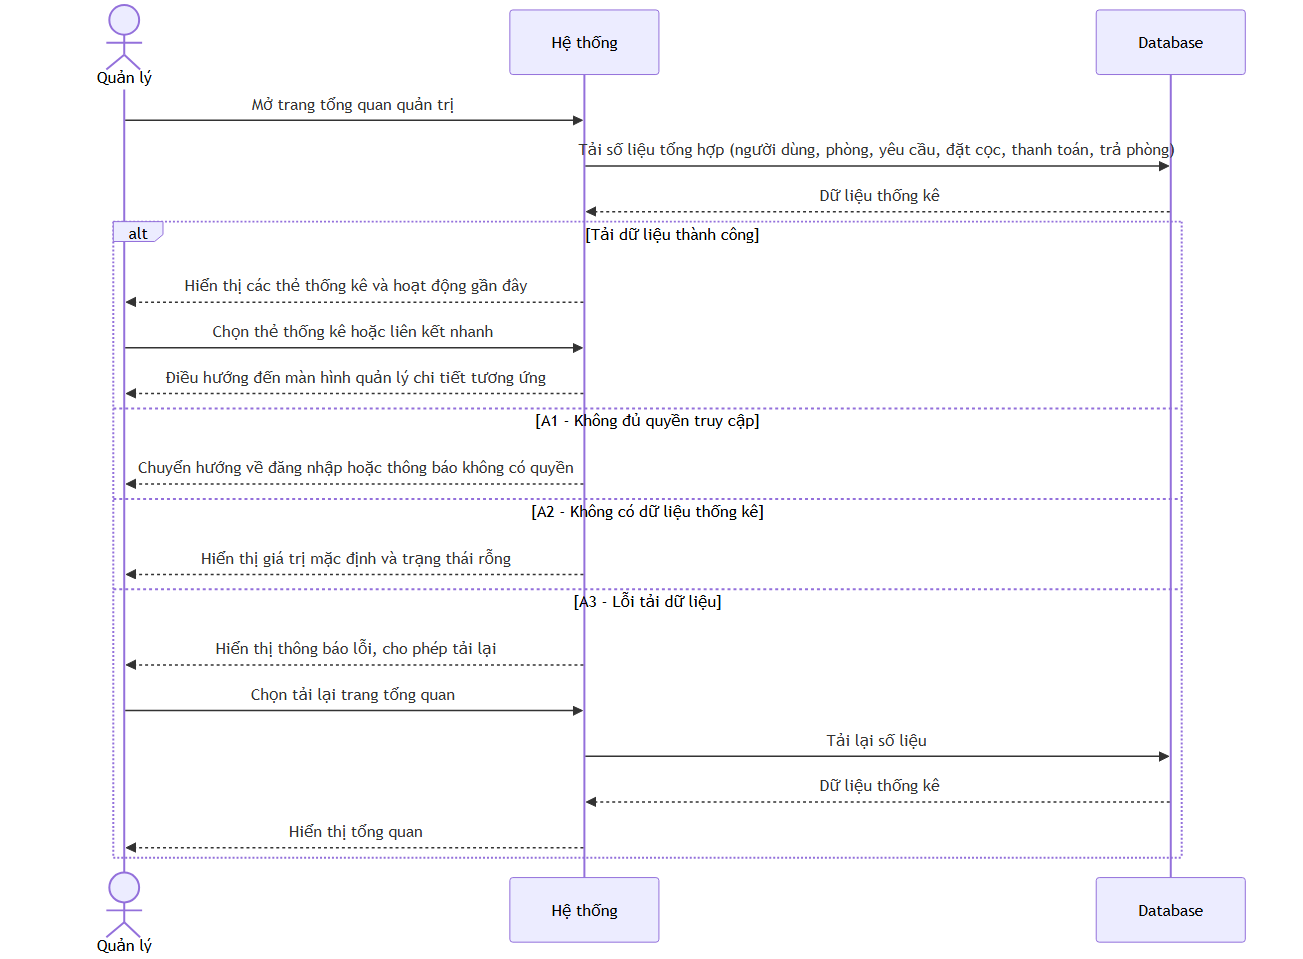
\includegraphics[width=\textwidth]{images/sequence_diagrams/SUC21_TongQuanQuanTri.png}
    \caption{Sơ đồ tuần tự -- SUC21: Tổng quan quản trị}
    \label{fig:seq-suc21}
\end{figure}




\newpage
\section{Cài đặt hệ thống}
\label{sec:implementation}

\subsection{Ánh xạ giữa các module triển khai và các SUC}

\begingroup
\small
\setlength{\LTleft}{0pt}
\setlength{\LTright}{0pt}
\begin{longtable}{|p{4.0cm}|p{2.9cm}|p{8.1cm}|}
\caption{Ánh xạ giữa các module đã triển khai và các SUC tương ứng}\label{tab:implementation-suc-mapping}\\
\hline
\textbf{Module triển khai} & \textbf{SUC liên quan} & \textbf{Mô tả triển khai} \\
\hline
\endfirsthead

\hline
\textbf{Module triển khai} & \textbf{SUC liên quan} & \textbf{Mô tả triển khai} \\
\hline
\endhead

\textbf{Authentication Module} & SUC1, SUC18, SUC19 & Hỗ trợ đăng ký tài khoản, xác thực OTP qua email, đăng nhập, quên và đặt lại mật khẩu, đăng xuất, lấy thông tin người dùng hiện tại, cập nhật hồ sơ cá nhân, kiểm soát truy cập dựa trên vai trò (RBAC) và Angular route guards. \\
\hline
\textbf{Room Management Module} & SUC12, SUC13, SUC21 & Cung cấp chức năng danh sách phòng với khả năng lọc và tìm kiếm, xem chi tiết phòng, đồng thời hỗ trợ các thao tác tạo, cập nhật và xóa phòng. Module này bao gồm cả giao diện quản trị và giao diện tra cứu dành cho khách hàng. \\
\hline
\textbf{Bed Management Module} & SUC12, SUC13 & Cho phép quản trị viên tạo mới và cập nhật thông tin giường trong từng phòng, hỗ trợ trực tiếp cho nghiệp vụ quản lý phòng và giường của hệ thống. \\
\hline
\textbf{Rental Request Module} & SUC2, SUC3, SUC20 & Cho phép khách hàng gửi yêu cầu thuê phòng/giường sau khi hệ thống kiểm tra tình trạng còn trống. Staff và admin có thể xem danh sách yêu cầu, xem chi tiết và cập nhật trạng thái xử lý yêu cầu. \\
\hline
\textbf{Booking Module} & SUC2, SUC20 & Cung cấp giao diện xem danh sách đặt chỗ, xem chi tiết booking, thực hiện các thao tác liên quan đến booking và tạo booking mới, bám sát luồng đăng ký thuê và theo dõi trạng thái xử lý. \\
\hline
\textbf{Contract Module} & SUC7, SUC16, SUC17 & Hỗ trợ tạo, cập nhật và xem hợp đồng, đồng thời phục vụ các bước kiểm tra điều kiện lưu trú và quy trình nhận phòng/bàn giao phòng. \\
\hline
\textbf{Payment \& Deposit Module} & SUC4, SUC5, SUC6, SUC8, SUC9 & Bao gồm quản lý giao dịch, quản lý đặt cọc, duyệt hoặc từ chối đặt cọc, xử lý thanh toán, tính toán chi phí, đối soát cuối kỳ và thực hiện hoàn tiền khi cần thiết. \\
\hline
\textbf{Viewing Appointments Module} & SUC14, SUC15 & Cho phép khách hàng đặt lịch xem phòng, trong khi staff và admin có thể duyệt hoặc từ chối lịch hẹn cũng như ghi nhận kết quả sau buổi xem phòng. \\
\hline
\textbf{Real-Time Chat Module} & Không có SUC riêng & Được triển khai như một tính năng hỗ trợ giao tiếp giữa khách hàng và nhân viên trong nhiều luồng nghiệp vụ khác nhau. Chức năng chat thời gian thực, hộp thư quản trị và read receipts được bổ sung nhằm cải thiện tốc độ phản hồi, mặc dù chưa được mô hình hóa thành một SUC độc lập trong hệ thống sơ đồ hiện tại. \\
\hline
\textbf{User Management Module} & SUC19 & Cho phép admin quản lý tài khoản người dùng, bao gồm xem danh sách người dùng, xem chi tiết hồ sơ, cập nhật vai trò/trạng thái và thực hiện soft delete tài khoản. \\
\hline
\textbf{Branch \& Zone Module} & SUC13, SUC21 & Hỗ trợ tổ chức dữ liệu phòng theo chi nhánh và khu vực (zone), phục vụ chức năng tra cứu phòng và cung cấp ngữ cảnh dữ liệu cho dashboard quản trị. \\
\hline
\textbf{Admin Dashboard} & SUC21 & Hiển thị các thống kê tổng quan như số lượng người dùng, số lượng phòng, booking đang hoạt động, doanh thu và các yêu cầu đang chờ xử lý. \\
\hline
\textbf{Lodging Eligibility Module} & SUC16, SUC17 & Thực hiện kiểm tra điều kiện lưu trú và xử lý thông tin đánh giá trước khi khách hàng tiến hành nhận phòng. \\
\hline
\textbf{Customer Dashboard \& Profile} & SUC1, SUC20 & Cung cấp giao diện tổng quan cho khách hàng về booking hiện tại, các khoản thanh toán sắp tới và các thao tác nhanh; đồng thời hỗ trợ cập nhật thông tin cá nhân. \\
\hline
\textbf{Public-Facing Pages} & Không có SUC riêng & Bao gồm các trang công khai như About, Contact và Guidelines nhằm giới thiệu hệ thống, cung cấp thông tin liên hệ và các quy định dành cho người dùng chưa đăng nhập. \\
\hline
\textbf{Internationalization (i18n)} & Không có SUC riêng & Hỗ trợ chuyển đổi giữa tiếng Việt và tiếng Anh, đồng thời lưu lựa chọn ngôn ngữ của người dùng nhằm nâng cao khả năng tiếp cận giao diện mà không gắn với một SUC nghiệp vụ cụ thể. \\
\hline
\textbf{Cross-Cutting Technical Features} & Tất cả SUC & Bao gồm JWT authentication, rate limiting, middleware xử lý lỗi tập trung, HTTP interceptor, Angular route guards, tích hợp NgZone cho realtime synchronization, responsive layout và hệ thống kiểm thử Jest. Đây là các thành phần nền tảng phục vụ toàn bộ các SUC trong hệ thống. \\
\hline
\end{longtable}
\endgroup

Các SUC trong Bảng~\ref{tab:implementation-suc-mapping} được đối chiếu trực tiếp với các sơ đồ tuần tự đã trình bày trong Chương~3. Việc ánh xạ này bảo đảm rằng mỗi module triển khai đều có thể truy vết về một hoặc nhiều luồng nghiệp vụ đã được đặc tả trước đó.

\subsection{Triển khai theo các luồng nghiệp vụ chính}

\subsubsection{Xác thực, phân quyền và quản lý hồ sơ người dùng}

Nhóm chức năng này chủ yếu tương ứng với SUC1, SUC18 và SUC19. Ở tầng backend, module authentication chịu trách nhiệm xử lý đăng ký tài khoản, xác thực email bằng OTP, đăng nhập, gửi lại OTP, quên mật khẩu, đặt lại mật khẩu, đăng xuất và cập nhật hồ sơ cá nhân. JWT được sử dụng để nhận diện phiên đăng nhập, trong khi cơ chế RBAC được áp dụng nhằm kiểm soát quyền truy cập theo từng vai trò như customer, sale, accountant, manager và admin.

Ở tầng frontend, Auth Guard và HTTP Interceptor được triển khai để bảo vệ các route yêu cầu xác thực và tự động đính kèm access token vào các request gửi đến backend. Cách triển khai này giúp bảo đảm tính nhất quán trong toàn bộ quy trình xác thực từ giao diện người dùng đến hệ thống backend, đồng thời tạo nền tảng bảo mật cho các chức năng khác như quản lý phòng, đặt cọc và thanh toán.

\subsubsection{Quản lý phòng, giường, xem phòng và yêu cầu thuê}

Nhóm chức năng này bao phủ các SUC12, SUC13, SUC14, SUC15, SUC2, SUC3 và SUC20. Module quản lý phòng và giường cho phép quản trị viên tạo, cập nhật, xóa và tra cứu phòng/giường dựa trên các tiêu chí như chi nhánh, khu vực, trạng thái và nhiều bộ lọc khác. Dữ liệu này được tái sử dụng trong giao diện khách hàng nhằm hiển thị các phòng còn trống, thông tin chi tiết phòng, hình ảnh và tiện ích đi kèm.

Quy trình xem phòng và đăng ký thuê bắt đầu khi khách hàng tìm được phòng phù hợp và tiến hành gửi yêu cầu thuê hoặc đặt lịch xem phòng. Staff và admin có thể xem xét yêu cầu, xác nhận lịch hẹn và ghi nhận kết quả sau buổi xem phòng. Trạng thái xử lý của các yêu cầu được đồng bộ lên dashboard khách hàng, cho phép người dùng theo dõi tiến trình xử lý theo thời gian thực.

\subsubsection{Đặt cọc, hợp đồng, thanh toán và thanh lý}

Nhóm chức năng này tương ứng với các SUC4, SUC5, SUC6, SUC7, SUC8, SUC9, SUC10, SUC11, SUC16 và SUC17. Sau khi yêu cầu thuê được phê duyệt, hệ thống tiếp tục xử lý các bước đặt cọc, tạo hợp đồng, thu các khoản phí ban đầu, kiểm tra điều kiện lưu trú và bàn giao phòng. Đây là giai đoạn quan trọng nhất trong quy trình nghiệp vụ vì liên quan trực tiếp đến doanh thu, vòng đời hợp đồng và các yêu cầu pháp lý trong quá trình lưu trú.

Hệ thống thanh toán và đối soát được triển khai theo hướng phân tách trách nhiệm rõ ràng giữa các vai trò. Staff và accountant chịu trách nhiệm xử lý thanh toán, theo dõi trạng thái đặt cọc, thực hiện billing định kỳ hàng tháng, tính toán chi phí cuối kỳ và xử lý hoàn tiền khi cần thiết. Các công thức hoàn tiền và khấu trừ được triển khai dựa trên các quy tắc nghiệp vụ đã được đặc tả trong phần use case tương ứng.

\subsubsection{Các tính năng hỗ trợ và mở rộng}

Một số thành phần như chat thời gian thực, dashboard quản trị, internationalization, các trang public và các cơ chế kỹ thuật cắt ngang không phải lúc nào cũng gắn với một SUC riêng biệt. Tuy nhiên, các thành phần này đóng vai trò quan trọng trong việc nâng cao trải nghiệm người dùng cũng như hiệu quả vận hành của hệ thống.

Chat widget và admin chat inbox hỗ trợ trao đổi nhanh giữa khách hàng và nhân viên trong các quy trình liên quan đến booking, đặt cọc, hợp đồng và thanh lý. Cơ chế internationalization cho phép giao diện chuyển đổi linh hoạt giữa tiếng Việt và tiếng Anh mà không ảnh hưởng đến logic nghiệp vụ của hệ thống. Các trang công khai như About, Contact và Guidelines hỗ trợ cung cấp thông tin cho người dùng trước khi đăng nhập, trong khi dashboard quản trị giúp theo dõi tổng quan hoạt động toàn hệ thống.

Về mặt kỹ thuật, các thành phần như JWT authentication, rate limiting, centralized error handling, route guards, tích hợp NgZone, Supabase Realtime synchronization, responsive layout và hệ thống kiểm thử Jest góp phần bảo đảm tính ổn định, khả năng mở rộng, khả năng bảo trì và tính an toàn của hệ thống.

\FloatBarrier
\newpage

% === file này không sửa gì vào nha, thêm ref ở file ref.bib

\cleardoublepage
\phantomsection
\addcontentsline{toc}{section}{Tài liệu tham khảo}
\nocite{*}
\bibliographystyle{unsrt}
\bibliography{ref}



\end{document}


